\begin{abstract}

The blockchain is a disruptive technology that enables the management of distributed workflows by automating the execution of complex processes. This system enables mistrusted entities to query and alter information without trusting a middle party, while providing a secure data storage in a decentralized scenario. In this thesis, we focus on an IT data supply chain scenario, where multiple actors negotiate a tenancy agreement for network virtualization. This process consists of service providers (SPs) requesting the embedding of specified virtual networks across multiple infrastructure providers (InPs). Since InPs are typically not willing to disclose detailed information about their internal network topologies and resources consumption/utilization, this has been show to directly hamper the efficiency of the service negotiation process. After observing how the blockchain can face the challenges encountered in supply chain processes and reviewing the related work on centralized and decentralized virtual network embedding (VNE) systems, we reason on why the blockchain is an appropriate approach for the described scenario. In order to enhance the VNE throughput, a brokerless system, that uses the blockchain, smart contracts and a VN partitioning algorithm based on the Vickrey auction model is designed and subsequently implemented. Finally, we further investigate the feasibility of our solution, by first analyzing the behavior of the introduced auction model in adverse conditions and by secondly evaluating the blockchain performance given different consensus protocols.
 
\end{abstract}

%*****************************************
\chapter{Introduction}
%*****************************************

Distributed workflows enable the automation of complex business processes by dynamically adapting the running instances in real-time. In a supply chain environment, since different parties perform multiple activities or tasks that alter the product information during its lifecycle, this automation could enhance the system efficiency. Thus, the supply chain cycle could benefit from a system that stores, shares and synchronizes the data as the events occur: a distributed ledger.

Blockchain (BC) is a type of distributed ledger, which has been considered one of the most promising and disruptive technologies of the last years. Many market-leading companies, and experts have referred to it as the "Next Generation of the Internet" \cite{JenClarck2017}, succeeding the World Wide Web era. After evaluating its potential benefits, different banks and enterprises, such as UBS, Microsoft or IBM, have already accomplished important investments in this innovative technology.

The revolution started in 2008, with the whitepaper publication by Satoshi Nakamoto \cite{nakamoto2008bitcoin}, who introduced a new digital payment protocol called Bitcoin. Satoshi Nakamoto was a name used by a person or group of people to first reference the performed work. Nowadays, its creator still remains unknown. One year later, a deployed software version based on the paper was launched, which enabled the use of Bitcoin to make trusted transactions between different peers on the Internet. This system was allocated in a blockchain, which is a public and distributed ledger that combined with cryptography models, removes the presence of middle-parties or intermediaries. In the case of Bitcoin, it eliminates the agents responsible for managing the money transactions, the banks.

Firstly, the blockchain architecture was restricted to only one application: online payments. However, after observing its main advantages in other use cases, an improvement of Bitcoin emerged: Ethereum \citep{buterin2014next}. By contrast, Ethereum extends the power of decentralized transactions with a Turing-complete contract system, which uses Ethereum scripts, also called smart contracts, to perform any computation. A smart contract can be generated with non-restrictive and user-friendly programming languages, allowing developers to easily benefit from them. Therefore, it brings the user the opportunity to develop their own applications. Smart contracts are implemented in decentralized apps, which in contrast to normal web apps, its back-end is not allocated to a central server. In other words, by using them in the blockchain, their content is shared and stored in a more distributed and decentralized manner.

\section{Motivation}

Nowadays, blockchain has become a topic receiving a close review in the business world. Thousands of articles, research papers and books, such as: How the technology behind bitcoin is changing money, business and the world \cite{tapscott2016blockchain} or Blockchain: Blueprint for a new economy \cite{swan2015blockchain}, are catching the public eye. Nevertheless, as it is an emerging technology, and thanks to smart contracts, a necessity to look towards new horizons exists.

Several scenarios are currently investigated from a blockchain perspective, e.g: candidate's voting or asset tracking \cite{abeyratne2016blockchain}. In the former, voters send signed and encrypted ballots to the blockchain contract, who immediately verifies them. Simultaneously, it also preserves confidentiality, since the ballot can only be emitted from its owner. In the latter, each physical asset could be encoded in the blockchain enabling a fast and transparent tracking. For instance, Everledger \citep{lomas2015everledger}, a startup company from London, tracks diamonds by storing each diamond's digital identity on the BC, in order to prevent diamond theft.

After examining different blockchain applications in real-world scenarios, we observe that the technology provides many advantages when users are willing to share and alter real-time data in a distributed, secure and transparent manner. In this thesis, we will focus on an application example, where multiple enterprises are willing to solve the major challenges faced during a supply chain cycle.

\section{Problem Statement and Contribution}

Supply chain management is the process of linking organizations through information flows, in order to achieve a competitive strength or advantage that maximizes the customer value. Since the activities involved, go from the design or development of a product, up to its return on investment (ROI), a good coordination between those is extremely needed.

Furthermore, enterprises currently handle a large amount of information. This leads companies to suffer from considerable issues, such as scalability, data security or communication. For this reason, most of these organizations rely on third parties, which help them on the mentioned problems. However, what if this process could be efficiently accelerated in a secure and decentralized manner? Here, is where blockchain could play a crucial role.

In this research, the focus will be on IT companies facing this dilemma. The scenario includes, on one side, different customers, and in the other, organizations acting as providers. For example, eBay, one of the biggest multinational e-commerce corporations, acts as an intermediate for the product's purchase-sale. Therefore, eBay is responsible for managing the whole data. Nevertheless, can a user/company always safely trust third-parties? Why not distributing these privileges among multiple users, which cooperate for handling such complex tasks?

To prove this, in this thesis, we thoroughly investigate a service negotiation cycle, in which different service providers (SPs) are willing to embed virtual nodes across multiple InPs, in order to provide wide-area network services \cite{dietrich2015multi}. This process is called network virtualization or network slicing, in which typically, the brokers, named VN Providers (VNPs) are responsible for performing the service negotiation that enables the VN embedding. Nevertheless, infrastructure providers are not willing to publicly disclose detailed information about their internal network topologies and resources consumption/utilization, and hence to share this information with the VNPs.

For this reason, we further examine whether blockchain can enhance the process, by removing the presence of these third-parties (VNPs), while maintaining a coordinated process that ensures a secure storage of data. This negotiation will be based on a time-limited auction, where each virtual network request automatically creates a new smart contract on the blockchain that enables the bidding of the requested resources by the SP. In addition, a decentralized application, which guides users through the network virtualization process and directly interacts with the blockchain will be deployed.

Therefore, a good question for the thesis could be: How blockchain enhances the distribution of workflows between unknown parties while providing an efficient and secure environment? Exemplifying workflows, with the network slicing scenario.

\section{Outline}

This thesis is structured as follows. In chapter \ref{ch:background}, relevant background information about the blockchain evolution, the network virtualization concept and the different auction mechanisms, is provided. Subsequently, in chapter \ref{ch:relatedwork}, an overview of existing applications that integrate blockchain solutions for improving the supply chain management efficiency is given. Afterwards, a comparison of the related work on the multi-provider virtual network embedding is performed. Based on the observed problems and challenges, in chapter \ref{ch:design}, a conceptual design of a multi-provider virtual network embedding approach using blockchain is introduced. In chapter \ref{ch:implementation}, the implementation of the proposed brokerless system, together with the fundamental smarts contracts that ensure the system functionality, are presented. In chapter \ref{ch:evaluation}, the efficiency of the defined brokerless VNE system is evaluated. Lastly, in chapter \ref{ch:closure}, the conclusions, the main contributions and the possible future work of this thesis, are summarized.


%*****************************************
\chapter{Background}
\label{ch:background}
%*****************************************

In this section, an overview of the blockchain technology evolution is provided. It starts with the 1st blockchain generation related to cryptocurrencies, with Bitcoin as a leading representative. Then, we investigate the 2nd generation, with the so-called smart contracts driven by the Ethereum platform. This extends the idea of money transfers, to any other application that can be writable as a piece of code.

Afterwards, the network virtualization concept will be introduced, in which resource negotiation between customers and providers is crucial. Due to this importance, a well-known public negotiation mechanism will also be presented, that is, auctions.

\section{Blockchain: A decentralized and distributed ledger}

A blockchain is a decentralized distributed ledger, which stores the entire history of transactions on the network. In other words, it is a simple database distributed among a network of computers, where each computer has an identical copy of this database. This contrasts with traditional centralized (e.g. SQL) databases that are controlled by a single entity. Thus, in a blockchain, there is no central server or agent in the middle of the communication. For example, imagine a scenario where a user wants to transfer money to another one, see Figure \ref{fig:CentralizedvsDecentralized}. In a centralized system, the transaction will go first to the bank, who will update its internal database and subsequently perform the operation. In contrast, in a decentralized system, each user is able to directly transfer the money, since it possesses an updated copy of the database. Another example to replace a centralized design could be in the healthcare environment. There, patient records are stored in multiple databases, which always leads to a costly exchange of information between them. In this scenario, the blockchain could improve the process, preserving patients confidentiality in a secure and decentralized manner.

\begin{figure}[bth]
	\myfloatalign
	{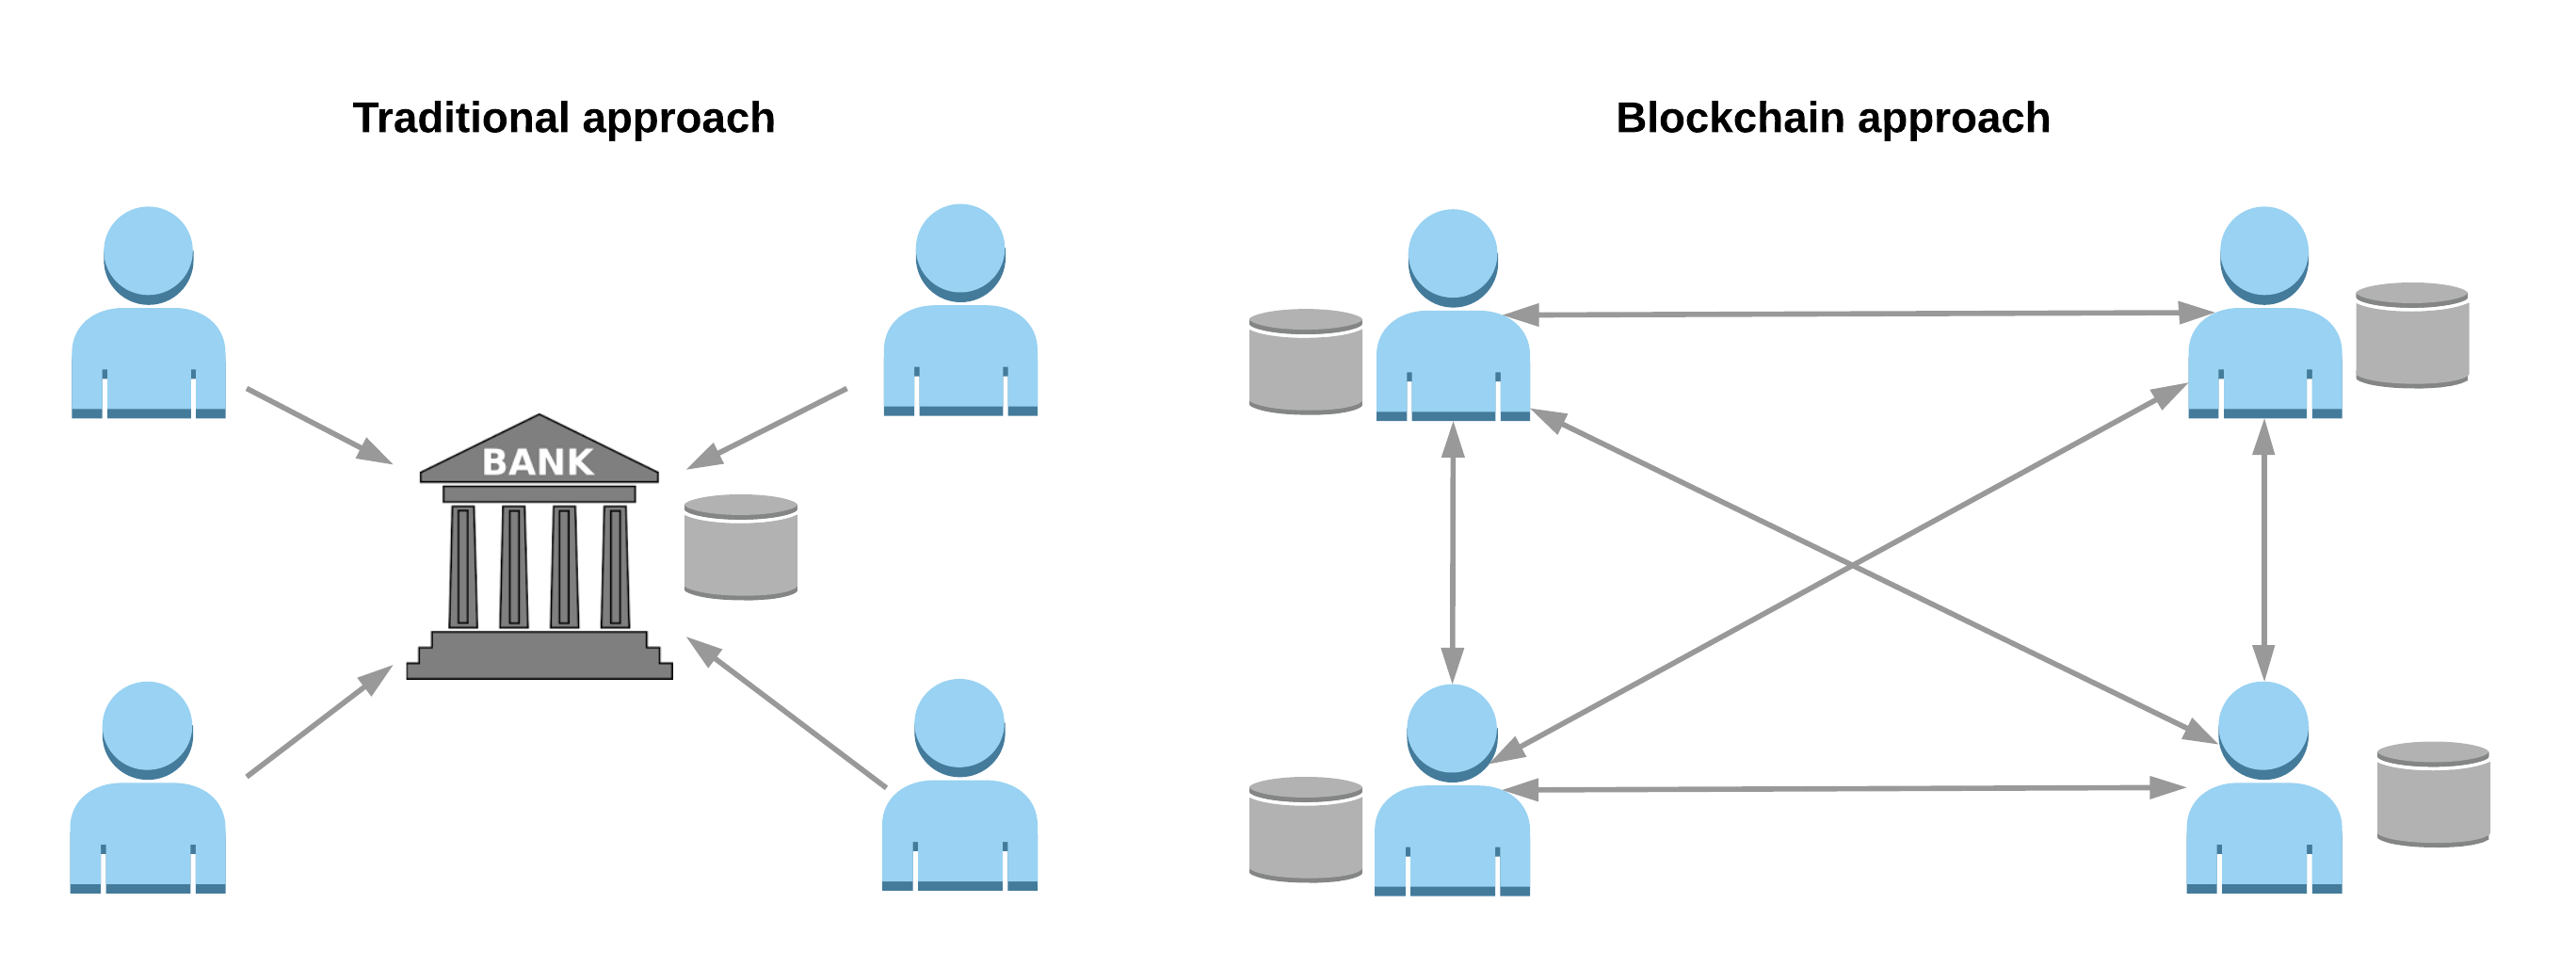
\includegraphics[width=0.4\linewidth]{gfx/cenVsDec}} \quad
	{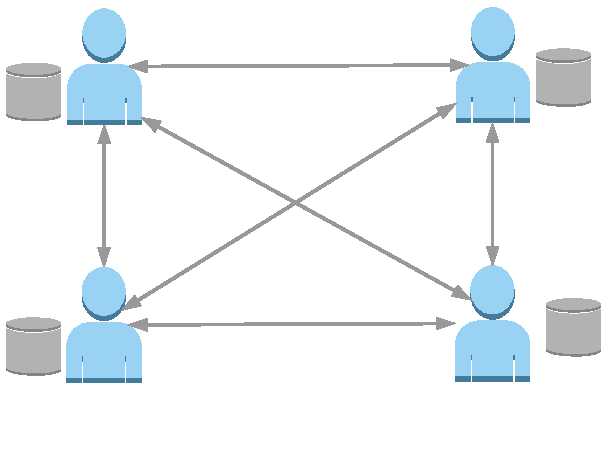
\includegraphics[width=0.4\linewidth]{gfx/cenVsDec2}} \\
	\caption{Centralized approach (traditional database) compared to a decentralized approach (blockchain).}
	\label{fig:CentralizedvsDecentralized}
\end{figure}

In the beginning, the terms Bitcoin and blockchain were sometimes interchanged, as these words were used to refer: (i) the technology, (ii) the protocol for making transactions and (iii) the cryptocurrency. Therefore, before continuing, one statement needs to be clear: \textbf{Bitcoin is a cryptocurrency that uses the blockchain technology and cryptocurrencies are just one of the multiple blockchain applications.} 

However, when a new technology appears, the first user's goal is normally to exploit its economic potential. For this reason, money transaction through cryptocurrencies was its first application. In the next subsection, we will understand what cryptocurrencies are, followed by an explanation of the Bitcoin's design architecture.

\subsection{Blockchain 1.0: Cryptocurrencies}

Cryptocurrencies are a variety of digital currencies pretending to work as a medium of exchange, such as Euro or USD. At of the end of January 2018, Coinmarketcap\footnote{\url{https://coinmarketcap.com/}}, a cryptocurrency market tracker, lists more than 1,400 cryptocurrencies with an aggregate value approaching USD 700bn. 

In addition, as the name suggests, they use cryptography to secure and verify its transactions. The main difference with traditional currencies is that they do not have any physical equivalent in the real world. Nevertheless, they can be used to pay goods and services, with the advantage of not being constrained by geographical or political borders. For example, GMO Internet\footnote{\url{https://www.gmo.jp}}, a Japanese company, will start paying parts of employees salaries in cryptocurrencies (Bitcoin).

In this thesis, we set aside whether cryptocurrencies can become true currencies or not, and also the political, social or economic impact. The only focus is on the technology behind it, as blockchain can be extended to much more than digital currencies. Thus, we will start from the genesis of the technology, with Bitcoin as its revolutionary innovator.


\subsubsection{Bitcoin}

Bitcoin took the world by surprise in 2008, after Satoshi Nakotomo's white paper publication \cite{nakamoto2008bitcoin} and later its software release. Bitcoin (BTC) is a cryptocurrency used for making secure transactions across peer-to-peer (P2P) networks. In addition, Bitcoin uses its own protocol that operates in an overlay network, the blockchain. An overlay network is built in the top of another network, in this case above the Internet application layer, which is controlled by its users.

From another point of view, cryptocurrencies ledgers can be interpreted as state transition systems, which change once a transition function (money transfer) is executed. In Bitcoin, the initial state is a list of not spent transactions, each containing the address supplying the BTCs, and the output is the receiver address along with the amount transferred. For this reason, Bitcoin is considered an unspent transaction output (UTXO) data model. For instance, in a scenario where user A wants to send 10 BTC to user B, the first state is A and B current balance, e.g. $\{A = 10, B = 20\}$. Afterwards, the transition function takes 10 BTC from A and insert it into B's account, generating a new state $\{A = 0, B = 30\}$. However, the problem arises if user A sends exactly the same payment to two different addresses (B and C) at the same time. This is the so-called \textit{double spending attack} and consequently, a transaction always needs to be verified by miners before being confirmed. 

\paragraph{Mining and Transactions} \label{mining_Transactions}

Miners are specific blockchain users, responsible for monitoring and verifying the transactions between users. The communication between these nodes is through a simple decentralized consensus protocol, which consists of multiple algorithms used by the miners in the Bitcoin network, such as the Proof of Work (PoW) consensus model.

Therefore, Bitcoin needs to combine its chains with a consensus protocol, in order to synchronize the order of all transactions among the users. In particular, new transactions are stored in the last block of the blockchain, and a new block is mined on average every ten minutes. Over time, this creates an ever-growing chain of blocks, which are constantly updated. Thus the name: blockchain. Additionally, a complete history of the transactions is kept, so everyone can verify the last money movements. For instance, a blockchain can be compared to an endless domino game, where all the pieces are placed in vertical one after the other. Each of these pieces references the previous block, and if one block is removed (e.g. transaction error), all the subsequent ones will be affected. Hence, as miner's task is not simple and requires computational power, these are economically rewarded if they are the first block solvers.

Apart from a list of transactions, each Bitcoin block contains a \textbf{block header}, whose hash is stored in the next block in order to maintain a consensus. Figure \ref{fig:Bitcoin Blockchain mining} shows how transactions are bundled into blocks, where each block header contains:

\begin{figure}[t]
  	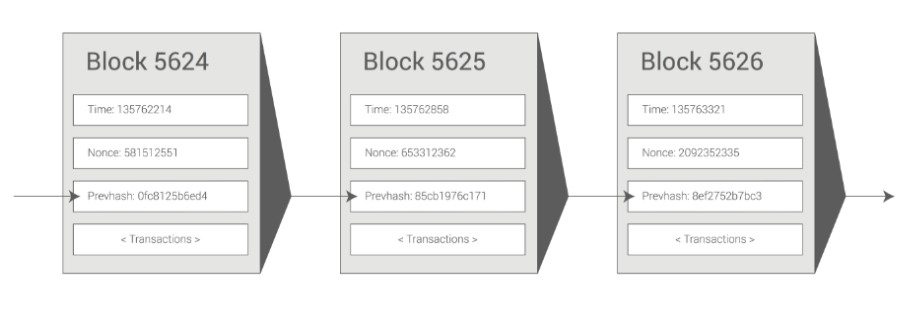
\includegraphics[width=1\linewidth]{gfx/mining}    
  	\caption{Bitcoin blockchain structure. Adapted from \citep{hans2017blockchain}.}
  	\label{fig:Bitcoin Blockchain mining}
\end{figure}

\begin{itemize}
	\item A timestamp, to identify when the event occurs.
	\item A nonce, which is an arbitrary number used for the miner to create the block header.
	\item The previous block header hash, to keep track of already added blocks.
	\item A block version number that indicates the validation rules used.
	\item A Nbits field, whose value should be higher than the block's header hash (later explained).
	\item A list of all the transactions that have been created since the previous block. To save storage, this transaction list is typically stored in a binary tree hash, named the Merkle tree \citep{merkle1987digital}.

\end{itemize}

Furthermore, in Bitcoin, each block and transaction is restricted to a size of 1MB and 250-300bytes respectively, and for a block being valid it needs to satisfy the following requirements:

\begin{itemize}
	\item Previous block referenced exists.
	\item Block's timestamp is greater than previous block one.
	\item The \textit{Proof of Work} in this block is valid.
	\item Exit if any transaction from the transaction lists returns an error.
	\item If all previous steps confirmed, the state is stored at the end of the block and return true.
\end{itemize}  

In the third step of the block validation process, appears the term \textit{Proof of Work}. Bitcoin uses the \textit{Hashcash} algorithm, to prove that a block miner spent some computational time creating a block, see Equation \ref{eq:proofOfWork}. More precisely, Bitcoin protocol demands that miners find a valid block header $B_h$ formed by a random value ($c$) and a nonce ($x$), whose cryptographic hash (e.g $SHA256$) is less than a \textit{target} value (a non-encoded version of Nbits). This value is obtained from the blockchain difficulty $d$. Then, the only way to create a valid block is simply trial and error until a valid Proof of Work is generated. This consensus model is also used in other contexts, such as for limiting email spam or denial-of-service attacks (DoS).

\begin{equation} \label{eq:proofOfWork}
 F_d(B_h) = F_d( \,c,x \,) = \text{SHA256}( \, \text{SHA256}( \, c|x \,) \,)\, < \frac{2^{224}}{d}
\end{equation}

\begin{figure}[bth]
  \centering
  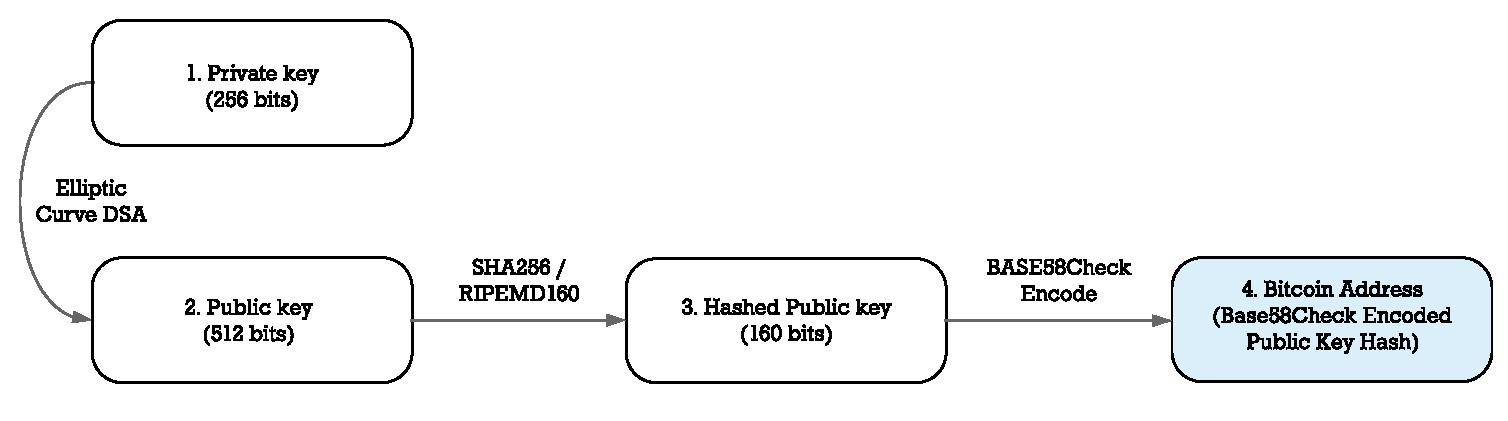
\includegraphics[width=0.9\linewidth]{gfx/bitkeys}    
  \caption{Bitcoin keys and addresses generation \citep{BitcoinKey2018}.}
  \label{fig:EthereumAccounts}
\end{figure}

\paragraph{Key management}

In Bitcoin, each user is identified by a single public address. The process to generate this address involves the following steps:

\begin{enumerate}
	
	\item A random private key is created, which must be kept secret since is used to sign transactions.
	\item A public key is generated from the private key, using the Elliptic Curve Digital Signature Algorithm \citep{johnson2001elliptic} (ECDSA). This key is used for verifying private key signatures.
	\item This public key is hashed using SHA-256/RIPEMD. Apart from size constraints, the reason for hashing the public key is that if there is a vulnerability in elliptic curves, user's money can still be safe, since only the hash is known.
	\item Finally, the public key is encoded in ASCII using Base58Check, whose output is the resulting Bitcoin address.
	
\end{enumerate}

Afterwards, users are able to send transactions using Bitcoin. For instance, in the last example where user A wants to send 10 BTC to user B. Firstly, the user creates a transaction to transfer 10 BTC to user address B. Secondly, he signs the transaction with his private key, attaching also his public one, and sends it to the blockchain. Once there, miners verify the signature using A's public key and check that its hash matches with user A address. If both, the signature and the hash, are correct, the transaction is accepted and added to the next block.

\subsection{Blockchain 2.0: Smart contracts} \label{smartContracts}

The Blockchain 1.0 had numerous limitations since essentially it only approaches the decentralization of money and payments. However, the architecture implemented by Bitcoin is extensible beyond financial uses cases. Therefore, in the following, we present another platform running in the blockchain.

\subsubsection{Ethereum}

In 2013, Vitalik Buterin, a Russian-Canadian programmer, released the Ethereum white paper \cite{buterin2014next}, where he describes an alternative platform running in the blockchain that allows building any kind of decentralized applications. One year later, Gavin Wood published the Ethereum yellow paper introducing the Ethereum Virtual Machine (EVM), i.e. a blockchain with a built-in programming language. Ethereum first started as a crowdfunding project to collect small amounts of money from a large number of users. Currently, it is the second most valuable cryptocurrency.

Furthermore, Ethereum extends the power of decentralized transactions with a Turing-complete contract system. A Turing-complete system can be proven mathematically to be capable of performing any computation, which allows developers to create its own programs. The code of these functions are written into the so-called \textbf{smart contracts} and executed by the Ethereum nodes, each using its Ethereum Virtual Machine (EVM).

\begin{lstlisting}[language=JavaScript,caption={Example of an Ethereum contract simulating a vending machine. The defined function returns a bottle of Coke if 2 \euro are inserted.},label={lst:CokeExample}]
contract Products {

	function getItem(bytes32 buttonPressed, uint amount) returns (bytes32 item) {
		if (buttonPressed == 'coke' && amount == 2) return coke;
 		return null;
	}
}
\end{lstlisting}

In essence, smart contracts are basically Ethereum scripts that whenever they are called, the function programmed inside of it is executed. A simple example of a contract is the logic inside a vending machine. For instance, a buyer wants a Coke bottle that costs 2 \euro. Once this buyer inserts 2 \euro and presses the button, a small program (contract) runs inside the vending machine and supplies the user with the Coke. In Listing \ref{lst:CokeExample}, we illustrate how this function could be defined in a smart contract.

Therefore, smart contracts allow writing customized functions in a few lines of code. Despite the fact that Bitcoin and Ethereum have similar features, such as decentralization or being transaction-based, Ethereum makes use of smart contracts, which potentially opens up its use cases. Bitcoin and Ethereum can be comparable to a calculator (one application) and a smartphone (multiple applications) respectively. In addition, there are other inequalities that need to be highlighted:

\begin{itemize}
	
	\item Ethereum's block time is shorter, specifically it is around 14s. In contrast, Bitcoin's mining time is around 10 minutes. As a consequence, Ethereum needs to handle a larger amount of transactions per second, which means that the network can easily get separated in different subchains. To solve this scalability issue, a new protocol from the new \textit{Proof-of-Stake} (PoS) mechanism, called  \textit{Casper}, has been recently proposed \cite{proofOfStake}.
	\item Thus, Ethereum pretends to move from the \textit{Proof-of-Work} to the \textit{Proof-of-Stake} consensus algorithm. In contrast to PoW, in which the miners that first solve a mathematical problem are rewarded, in PoS, validators propose and vote the next block. In this case, the voting power is directly proportional to the validator's stake (deposit) and to become validators, users need to lock up their ether into a deposit. Therefore, in PoS there are validators rather than miners.
	\item Bitcoin's blocks and transaction sizes are indicated in bytes, however, in Ethereum, this depends on the contract complexity. This complexity is expressed in terms of \textit{gas}, which is the amount of spent Ether used for executing contracts in the Ethereum blockchain. Ether, also called ETH, is the digital currency used by Ethereum. This contract gas used is later earn by the miner as a reward.
	\item Ethereum transactions, apart from the already mentioned Bitcoin fields, consists of (i) a transaction value in Ether, (ii) recipient address, (iii) data arguments and (iv) execution cost.
	\item Ethereum is account-based and not transaction-based.
\end{itemize}
In the last point, we observe that Ethereum introduces a new concept called accounts. These accounts are unique 20-byte addresses, each of them having a balance controlled by ethers (ETHs). In Ethereum, there are two types of accounts (Figure \ref{fig:EthereumAccounts}):

\begin{itemize}
	
	\item \textbf{Externally Owned Accounts (EOAs):} These accounts identify users and are controlled by the user's public and private keys. An EOA is the only account that can send transactions to other accounts, where a transaction in Ethereum is either sending ETHs or calling a contract account.
    \item \textbf{Contract accounts:} These accounts are responsible for storing smart contracts, whose code is executed once triggered.
\end{itemize}

\begin{figure}[bth]
  \centering
  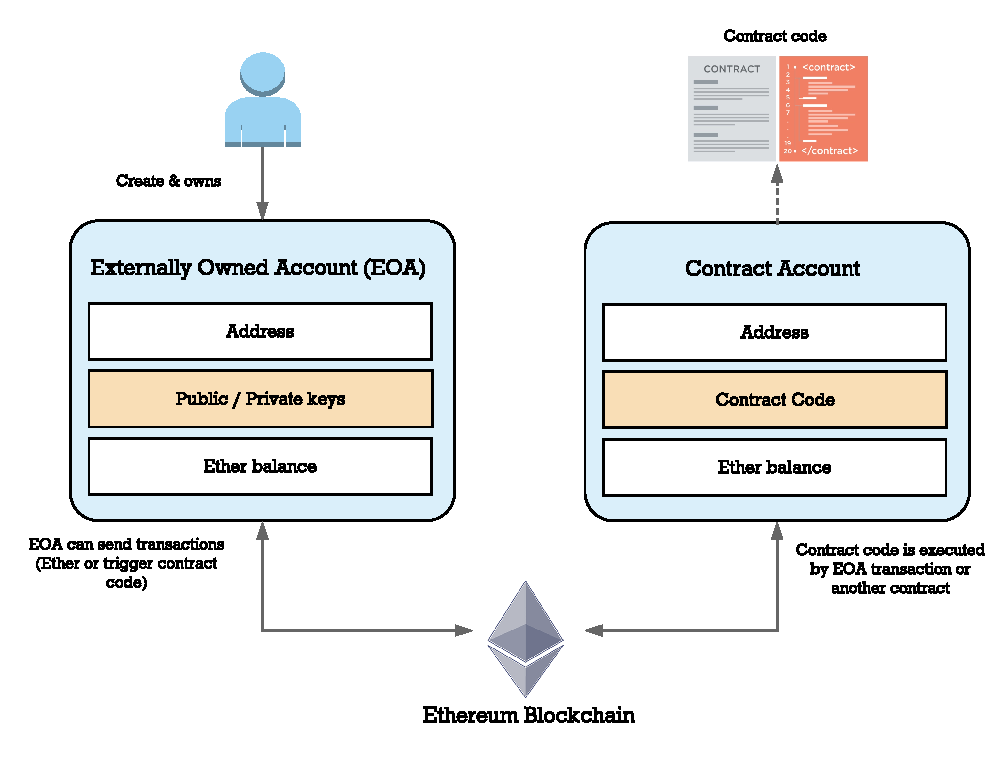
\includegraphics[width=0.6\linewidth]{gfx/ethereumAccounts}    
  \caption{Ethereum accounts: Externally owned accounts and contract 			accounts.}
  \label{fig:EthereumAccounts}
\end{figure}

In order to solve that a contract execution results in an infinite loop, Ethereum uses the term gas. For instance, when an EOA calls a contract account to transfer money, apart from the ether transferred, this spends an additional amount of ether (gas). In Equation \ref{eq:transFee}, we depict this transaction fee $F$.

\begin{equation} \label{eq:transFee}
	F = P \times L + V - R
\end{equation}

Firstly, the gas limit $L$ is the maximum amount of gas to spend on a transaction, which is by default 21000. Secondly, in Ethereum, the gas price $P$ is measured in units of Gwei, which is equivalent to $1e^{-9}$ ETH. Thirdly, the value $V$ is the amount of ether transferred to the other EOA. Fortunately, all unused gas $R$ during a transaction is refunded to the sender. Nevertheless, if a transaction returns an error, e.g: gas provided not enough to execute a contract, this provided ether will never be refunded. 

In conclusion, a smart contact is just an account containing code, which lives on the blockchain and allows developers to create their own decentralized applications. 

\subsubsection{Decentralized applications}

In the Ethereum white paper \cite{buterin2014next}, decentralized applications (dapps) are divided into three types. The first group includes financial applications, where users only manage money transactions, e.g. a customer paying the provider through a blockchain application. The second group is formed by semi-financial applications, in which money is involved but it is mixed with other requirements. For instance, an application where users receive incentives for computational problems solutions. And finally, in the third category, there are non-financial applications. For instance, an online voting platform providing a better transparency into elections, without compromising voter confidentiality.

Despite the blockchain is a secure technology, the created applications are constantly compromised to multiple attacks. This is because the majority of smart contracts are insecure, due to its code being prone to bugs. For example, in June 2016, the DAO\footnote{\url{https://ethereum.org/dao}}, which is a distributed autonomous organization instantiated on the Ethereum blockchain, was hacked. Due to a smart contract bug, the attack resulted in over 50 million dollars of cryptocurrency theft. Thus, smart contracts need to be protected against malicious attacks before being uploaded on the blockchain.

In the following section, an example application process currently performed by IT companies is presented.


\section{Network Virtualization} \label{networkvirtualization}

In the last years, network virtualization has started to grow in popularity since it enables simulating baremetal networks. These virtual networks, in contrast to physical networks, provide better flexibility, manageability and lower costs. 

Network virtualization handles two main concepts: node virtualization and link virtualization. The former implies sharing the node's physical resources, which are located in the substrate network (e.g: CPU, storage, memory), to multiple virtual nodes of the virtual networks. For instance, physical node A in Figure \ref{fig:networkvir_a}. The latter enables the transport of multiple virtual links in a single and shared physical link (Figure \ref{fig:networkvir_b}).

\begin{figure}[bth]
	\myfloatalign
	\subfloat[Network virtualization model.]
	{\label{fig:networkvir_a}%
	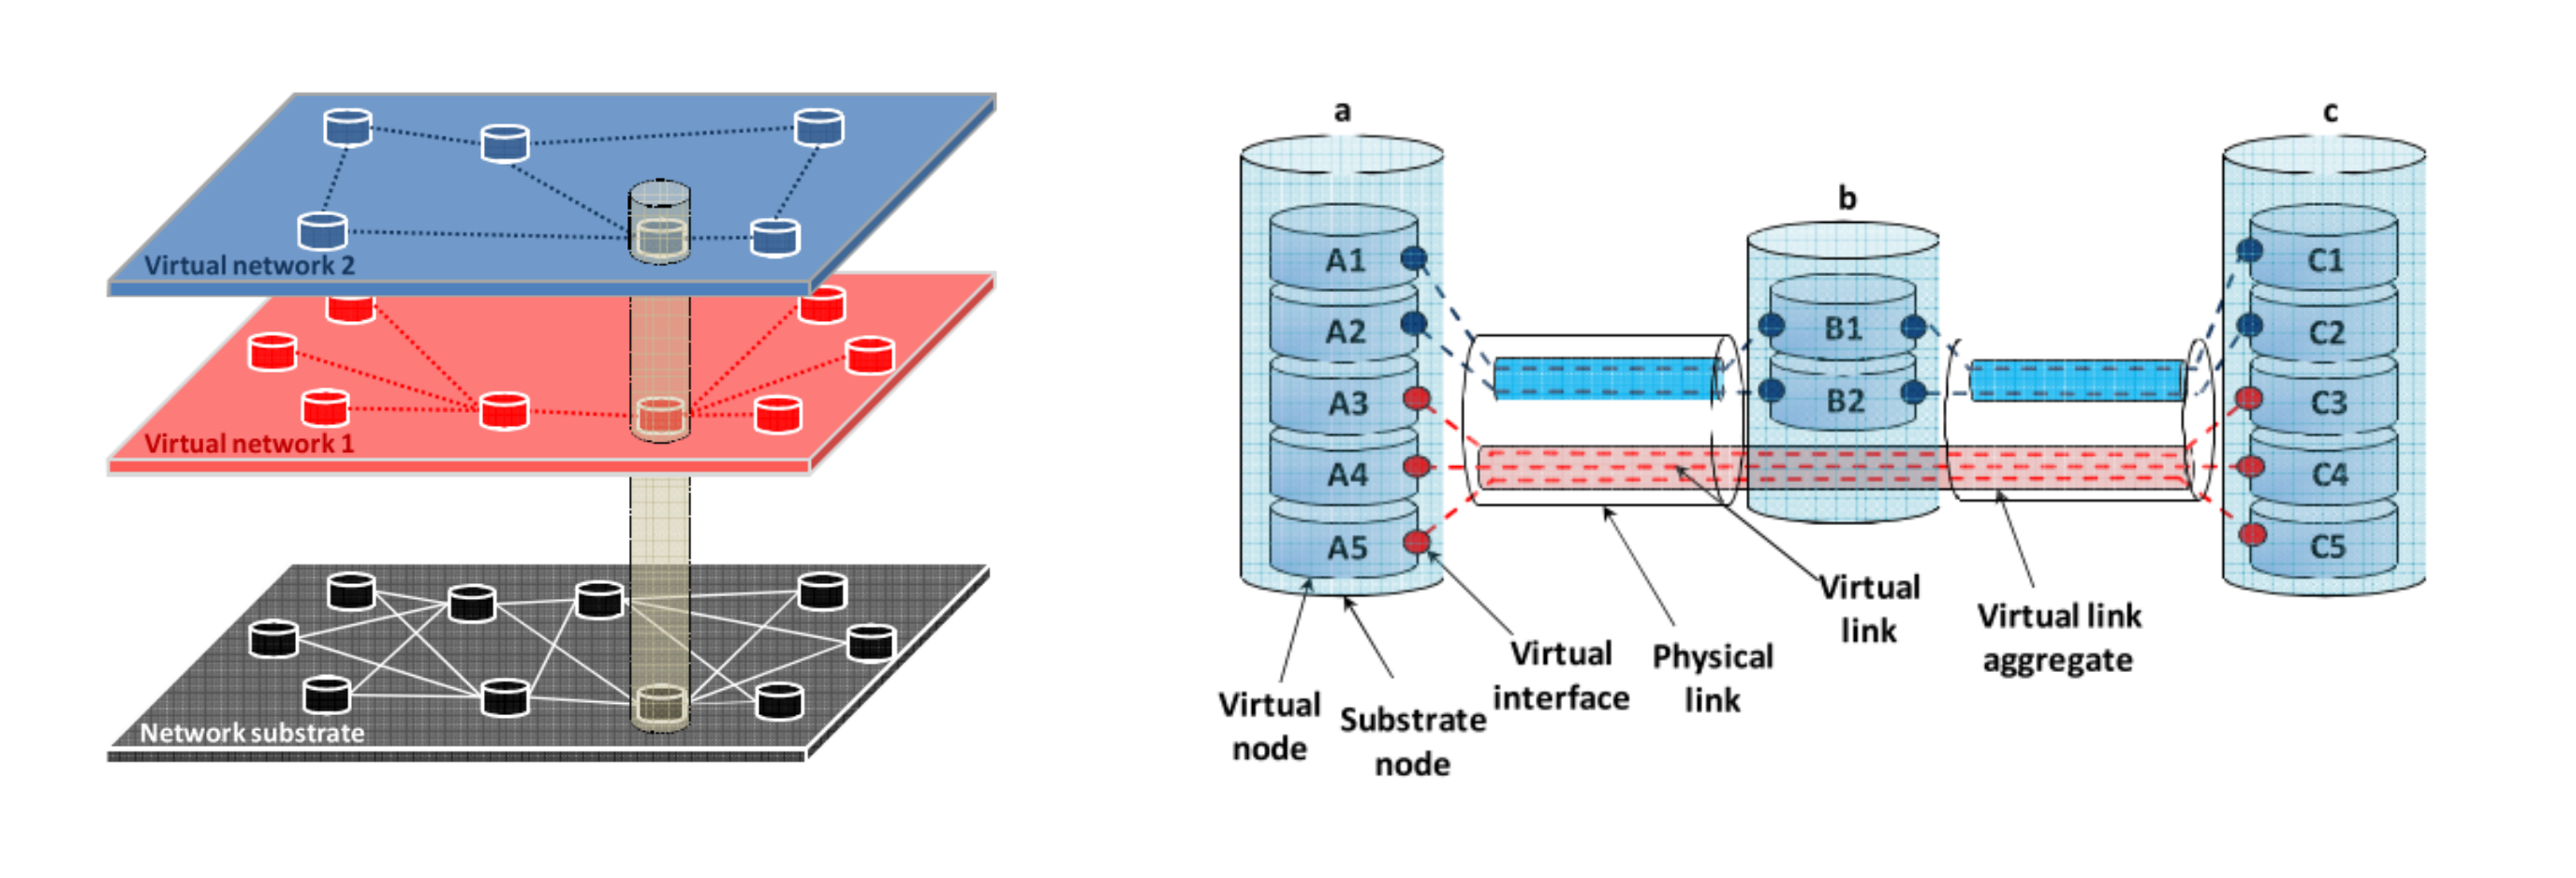
\includegraphics[width=0.48\linewidth]{gfx/networkvir}} \quad
	\subfloat[Network virtualization elements.]
	{\label{fig:networkvir_b}%
	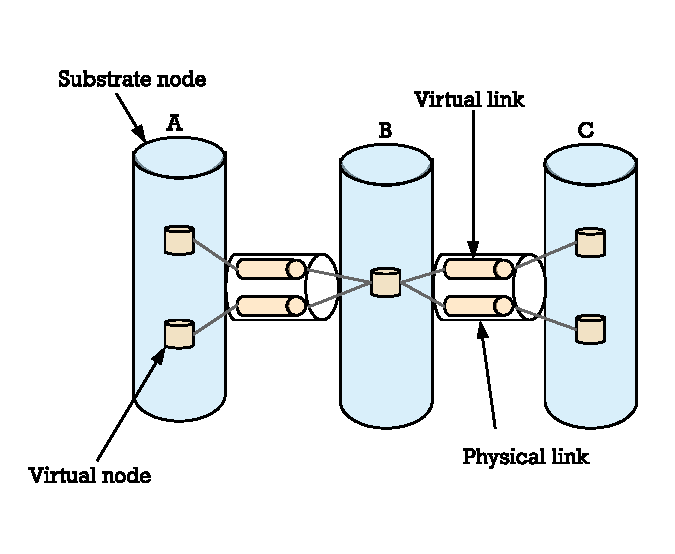
\includegraphics[width=0.48\linewidth]{gfx/networkvir2}} \\
	\caption{Network virtualization model and its basic elements. Adapted from \citep{carapinha2009network}.}
	\label{fig:networkvir}
\end{figure}

In the network virtualization process, there are two main actors (and one optional) participating:

\begin{itemize}
	
	\item \textbf{Infrastructure providers (InPs):} Infrastructure providers (e.g: Deutsche Telekom or Telefonica) deploy and manage the physical nodes, sharing efficiently its resources to the virtual network. For InPs, this results in a significant decrease in operational and technology investment costs \citep{dietrich2015multi}.
	\item \textbf{Service Providers (SPs):} Service providers lease virtual resources from infrastructure providers to create its customized virtual network, without the need to purchase physical network equipment.
		\item \textbf{Virtual network providers (VNPs):} Virtual network providers are brokers, which can optionally serve as intermediaries to perform the service negotiation between the InPs and SPs.
\end{itemize}

The network slicing process with the presence of a broker typically starts with the VNP obtaining the necessary network information from the SP. To optimize the software costs, the SP's virtual network request will be divided into groups of nodes (subgraphs). Afterwards, the modified network is transmitted to the multiple InPs, who are in charge of embedding the virtual nodes from the request in their physical resources. 

The presented process is coordinated by an actor, the VNP, who stores all the network information to successfully allocate the incoming resources. However, there are other approaches, where the InPs do not want to rely on a central entity, since its confidential information is being disclosed and hence, known by the VNP. Conversely, the SPs and InPs make use of consensus mechanisms to perform the virtual resources trading. Since no middle-party exists, this task is performed in a more decentralized manner. For this reason, in the following, we briefly investigate an open negotiation technique: the auctions.

\subsection{Auction Mechanisms} \label{auctionMechanisms}

Service negotiation has already been examined in many researchs, such as \citep{hausheer2005peermart}, \cite{ogston2002peer}, which have worked with diverse auctions platforms. An auction is a public negotiation method involving buyers and sellers that enables resource trading between peer-to-peer users. While the buyer's goal is to find the desired service at the lowest price, the providers or seller's goal is to sell the service at the highest "possible" price. Thus, an auction should provide fairness in terms of technical and economic efficiency, for both the buyer and the seller.

Firstly, auctions can be divided into (i) \textit{one-sided auctions} where only the buyers submit their bids (e.g: a painting auctioned in an art exhibition), or (ii) \textit{two-sided auctions} in which buyers and sellers submit their bids. Normally, when any of the two sides (buyer or seller) cannot perform a good estimation of the service, a one-side auction is preferred. This is the case in network virtualization, where the SPs are not aware of the InPs physical nodes availability. 

Secondly, the auctions can be (i) \textit{open-cry} auctions, where the bids are broadcasted to all users, or (ii) \textit{sealed-bid} auctions in which bidders first commit bid values in secret that are later revealed (e.g: physical envelopes). In our scenario, the InPs should bid in a confidential manner, because they are not willing to disclose their internal network cost models. From the different auction types, our focus will be on the most common \cite{coppinger1980incentives}: 

\begin{itemize}
	\item \textbf{English auctions}, also called \textit{open-cry ascending-price} auction, is the classic bidding mechanism where the seller first sets a minimum starting value (reserve price), which buyers should overcome. Then, these buyers start to offer higher prices until nobody wants to offer a greater one. However, due to the competition, this auction model can result in a long process (e.g. low reserve price compared to real value) where users pay huge amounts.
	\item \textbf{Dutch auctions} are similar to the English auctions, but on the contrary, they are \textit{open-cry descending-price} auctions. In this model, seller fixes a maximum value which is reduced slightly over time. Once a buyer accepts a price, the auction will finish. Nevertheless, to prevent ending with low prices for the sellers, they also establish the mentioned reserve price, which will be the minimum accepted amount. Dutch auctions are faster than the English ones, but buyers will also end up paying more to ensure that they win.
	\item \textbf{Vickrey auctions} has the particularity of corresponding to a \textit{sealed-bid second-price} auction \cite{vickrey1961counterspeculation}. Since it is sealed, during the bidding time buyers do not know other bids and eventually, how the auction is evolving. In addition, the Vickrey auction corresponds to a second-price tender. This means that like standard auctions, the bidders will offer a price for the service, and the highest bid will win. Nevertheless, this service will be rendered at the second highest value. For example, imagine a bidding for product A, where the winner has bidden $\{A = 15\}$ and the second highest bid is $\{A = 10\}$. Then, this winner ends-up paying only $\{A = 10\}$. In addition, it is shown that a Vickrey auction is strategy-proof, meaning that each bidder quotes the true cost of the service, and if they do so, the resulting total values are maximised  \cite{vickrey1961counterspeculation}. From the bidder's point of view this means that he can safely bid the real value, knowing that if he wins, he will pay less than his bid. Thus, a Vickrey auction compared to English and Dutch auctions, is considered a fair-price system since it provides a reasonable price to the buyer by motivating bidders to bid truthfully.
	\item \textbf{Reverse auctions} as the name states, buyers and sellers roles are switched. In contrast to ordinary auctions, where buyers compete to obtain an asset, in reverse auctions, sellers compete to gain a business. In other words, the seller bids for his own services, which finally, are given to the supplier offering the lowest price. For example, in the network virtualization process, InPs bid for their physical nodes, and afterwards, the SP leases the most economical ones.
\end{itemize}

Lastly, after reviewing the preceding analysis, a \textbf{\textit{one-sided reverse Vickrey}} auction seems to be the most suitable for a brokerless virtual network embedding since it provides confidentiality and the biggest aggregate profit among sellers and buyers. This will be later investigated in chapter \ref{ch:design}.

\section{Summary}

The blockchain is a transparent, secure and robust system where users are in charge of their own accounts and transactions. Beyond money transfer, which started with Bitcoin, the blockchain technology can be used as a software connector in multiple scenarios. Due to smart contracts, arbitrary applications could be implemented in the context of Ethereum blockchains, enabling developers using the blockchain concept in their own environment. In the next chapters, we will investigate a multi-provider virtual network embedding scenario where infrastructure providers are not willing to disclose internal network cost models.

%*****************************************
\chapter{Related Work}
\label{ch:relatedwork}
%*****************************************

In the following, we explore some of the noted challenges that organizations encounter during their supply chain management (SCM) process, and how they currently approach these issues. Then, we introduce a recent application in manufacturing, to demonstrate how blockchain could improve SCM efficiency. Henceforth, we focus on a particular supply chain management example: virtual network embedding across multiple InPs. A comprehensive overview of related work on already implemented centralized and decentralized frameworks is also presented. Finally, we first enumerate the main blockchain benefits observed from the SCM manufacturing application point of view, and secondly, we analyze the pros and cons of the existing VNE related work, in order to observe the problems and limitations that need to be addressed in our thesis.

\section{Blockchain in Supply Chain Management}

In the last years, managing the information during the lifecycle of a product represented a major challenge for many companies \citep{karkkainen2003product}, \citep{tuttle2002you}. This product information is constantly changing and in addition, it has to be accessible by different entities. As a consequence, this problem results in high costs for companies. 

Typically, companies approach the problem by (i) storing and maintaining the data into their company-specific infrastructures, which is then communicated to the other supply chain partners, or by (ii) sharing this data in a centralized database. In the former, each enterprise creates its own copy of the product data and uses their own protocols and procedures. As a consequence, plenty of asymmetries are found, which ends up reducing the benefits of knowledge or data sharing. In \citep{lee1992managing} and \citep{fiala2005information}, an inadequate definition of customer services, poor coordination or organizational barriers are named to be some of the pitfalls that these users suffer from. On the other hand, the latter is a great solution as long as the companies trust the party who is maintaining the database. However, what if they are not willing to place this intermediary on their operations? Here, we foresee that blockchain could improve the process supplying data distribution and storage among these companies.

Apart from the supply chain, \citep{heikkila2002supply} states another relationship between suppliers and customers, the Demand Chain Management (DCM), where we predict that blockchain could also play a significant role. In a DCM, the aim is to provide a customer service at the least cost. Hence, the suppliers need a real-time visibility of customer situations and needs. The main difference is that in SCM, the stakeholders wait to receive the order for proceeding with a product (push), whereas in DCM the suppliers observe and immediately operate in user's petition (pull) \citep{wust2017you}. Currently, companies such as Everledger or Skuchain, offer blockchain services to manage and improve the supply chain performance.
 
In the following, we present a blockchain application that stores and distributes the product information during its lifecycle.

\subsection{Blockchain Ready Manufacturing Supply Chain} \label{manufacturing}

Product lifecycle management (PLM), is a process that involves different stages \citep{stark2015product}, in which multiple parties modify the product's data, see Figure \ref{fig:supplyChain_a}. In this application \citep{abeyratne2016blockchain}, each actor interacts with a user interface connected to the product's data from the blockchain. These products are created in form of rules (smart contract) so that only specific users can access or modify them. In this authentication process, parties must authenticate themselves signing the requests with their private keys. 

\begin{figure}[bth]
	\myfloatalign
	\subfloat[Product Lifefcycle Management (PLM) stages.]
	{\label{fig:supplyChain_a}%
	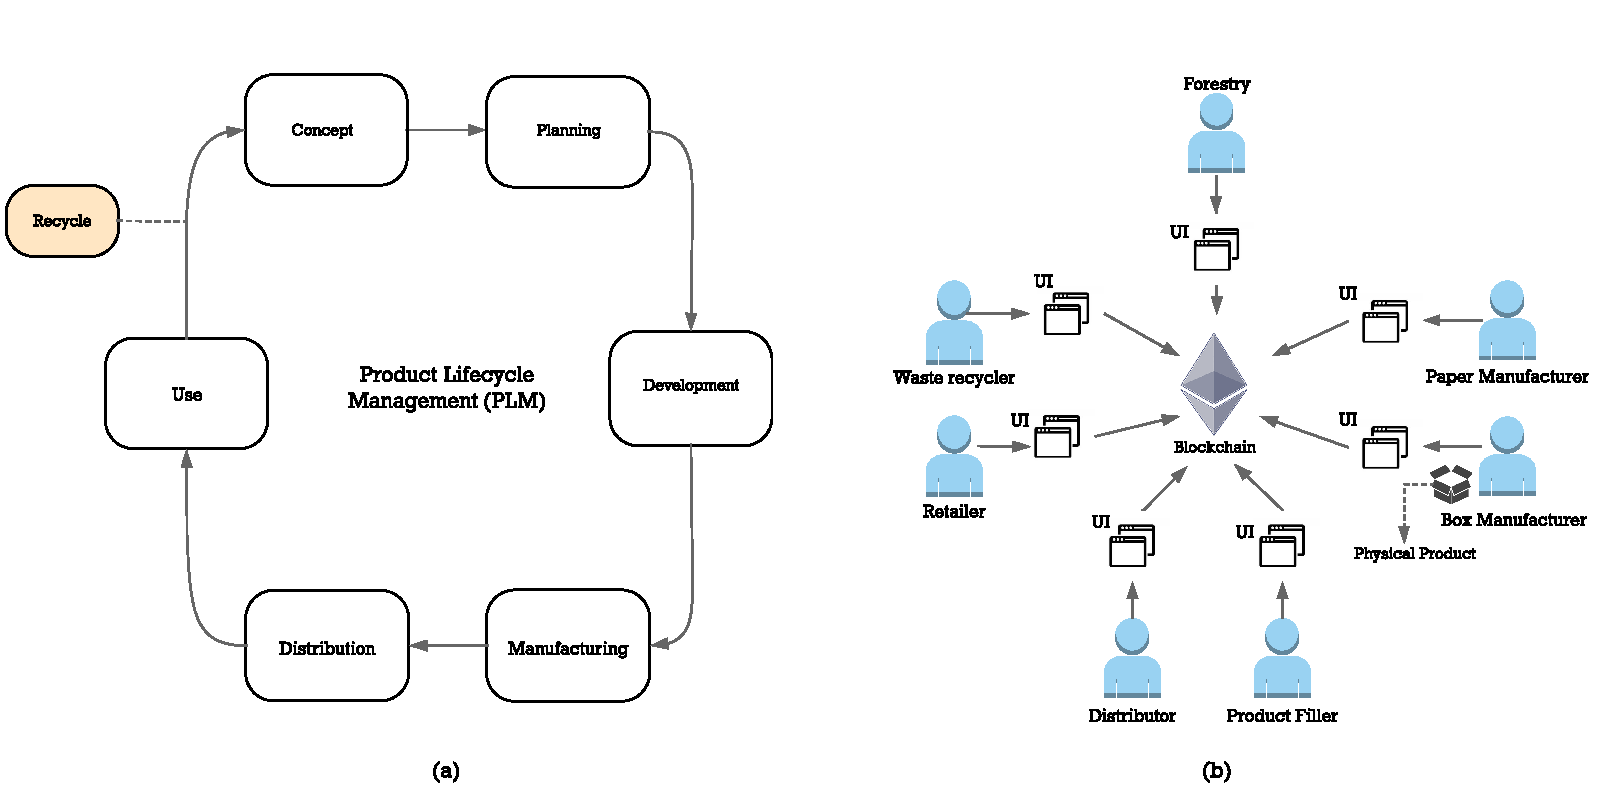
\includegraphics[width=0.48\linewidth]{gfx/supplyChain}} \quad
	\subfloat[Cardbox example.]
	{\label{fig:supplyChain_b}%
	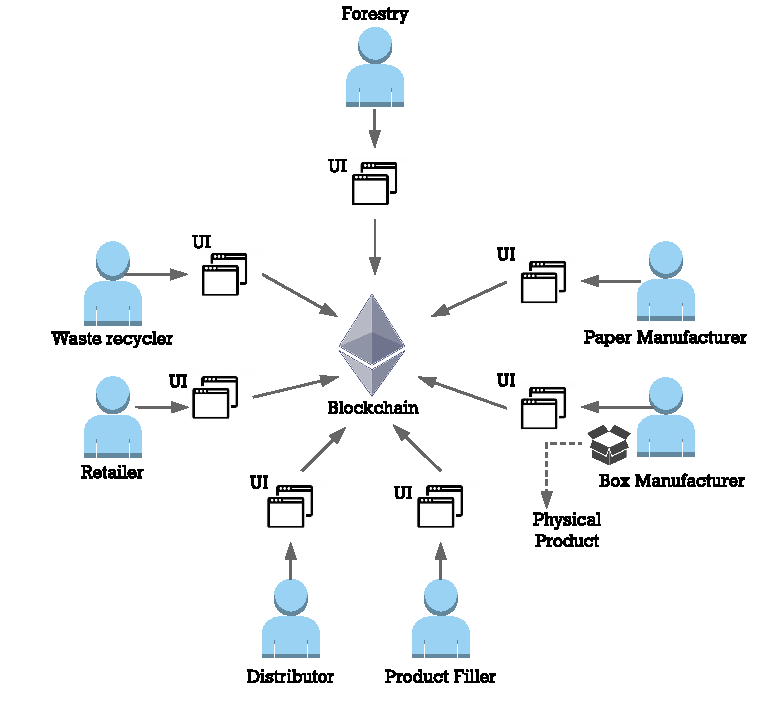
\includegraphics[width=0.48\linewidth]{gfx/supplyChain2}} \\
	\caption{Product Lifefcycle Management (PLM) stages and cardbox blockchain application example \citep{stark2015product}.}
	\label{fig:supplyChain}
\end{figure}

During the lifecycle management, a product is owned by an entity, such as the distributor. Moreover, when a product is transferred to another actor (e.g. from a distributor to a consumer), both parties sign a contract that updates the product's ownership, to ensure that only the granted users modify the contract.

At the end of \citep{abeyratne2016blockchain}, an example that better explains the mentioned approach is presented. The application consists of the product lifecycle of a cardboard box, starting from the trees cut down until the box is recycled. In Figure \ref{fig:supplyChain_b} an overview of the implemented design is presented. In this process, different actors are entailed. For instance, the box manufacturer first receives the physical object and then signs a contract to gain the product's access. Afterwards, he is allowed to alter it (e.g. modify the box quality), through the user interface. Once finished, he transfers the package (signed) to the next actor, in particular, the product filler, who follows the same steps.


\section{Network virtualization}

In the last years, many investigations in network virtualization have been conducted by different authors \citep{houidi2011virtual}, \citep{zhu2008cabernet}, \citep{chowdhury2009virtual}. Among those, it is important to highlight topics such as the trade-offs between single \citep{chowdhury2009virtual}, \citep{houidi2008distributed} and multi-provider VNE \citep{dietrich2017multi}, or the different techniques and algorithms used for achieving VN efficiency. Typically, they decompose the VNE into two tasks: VN partitioning and VN segment mapping \citep{fischer2013virtual}. 

Each of these studies proposes new interesting features compared to the prior research. Nevertheless, in this thesis, we will not contrast the different architectures (e.g. between a single or multiple InPs) or discuss the various VN partitioning and mapping algorithms. The main goal of this work will be to explore an existing network virtualization scenario, in particular, multi-provider VNE applications suffering from the limited information disclosure problem \citep{dietrich2017multi}, \citep{zaheer2010multi}, \citep{esposito2013general}, \citep{chowdhury2010polyvine}.

\subsection{Multi-Provider Virtual Network Embedding with Limited Information Disclosure}

To deploy wide-area networks, service providers are willing to embed virtual resources across heteregeneous domains belonging to different infrastructure providers. As a result, the system avoids being restricted to a single provider topology, which provides at the same time better efficiency. This process, also named inter-domain VNE\footnote{Inter-domain is between multiple InPs and intra-domain is inside a single InP.}, is descomposed in three main tasks \citep{chowdhury2010polyvine}:

\begin{itemize}
	\item \textbf{VN request partitioning}: Divide the virtual network into groups of virtual nodes (subgraphs), such that virtual node and link requirements are satisfied, minimizing at the same time the software costs of the virtual network setup.
		\item \textbf{Inter-connection between subgraphs}: Establish paths between the previously created subgraphs.
	\item \textbf{VN segment mapping}: Embed the virtual resources (subgraphs) to the InPs physical nodes.
\end{itemize}

Furthemore, in such scenarios exists two types of communication \citep{zaheer2010multi}:

\begin{itemize}	
    \item \textbf{Horizontal communication} is the one established between infrastructure providers to guarantee the most efficient end-services. These relations can be: \textit{public relations} established using a market mechanism (e.g: an auction), or \textit{private relations}, which are previously arranged because the InPs already know each other. In both cases, the relation arises from the need to negotiate and cooperate to serve the SPs.
	\item \textbf{Vertical communication} emerges from the negotiation between SPs and InPs, in which the former is willing to lease virtual resources from the latter. This communication is typically facilitated by a third party (VNP).
\end{itemize}

One of the main challenges of inter-domain VNE, is that InPs are not willing to broadcast their resources information (e.g: nodes availability, cost) or their network topology to the outside world \citep{dietrich2015multi}. Thus, the virtual resources need to be allocated in a constrained and limited scenario (LID). And if that was not enough, this InP's data is crucial to perform the partitioning of resources, in order to optimize the network software costs.

\subsubsection{Centralized Slice Embedding}

In \citep{dietrich2015multi}, a centralized VNE framework is implemented (Figure \ref{fig:multiprov_a}). There, the mentioned LID partitioning problem is approached through a VPN, who accesses public information that is not considered confidential by the InPs:

\begin{itemize}
	\item \textbf{Virtual resources availability}: In this case, virtual resources examples are obtained from Amazon EC2 \cite{amazonEC2}, which announces the attributes (CPU, memory, cost) of different instances types.
	\item \textbf{Substrate network topology}: Most of network's topology information is treated confidentially for the InPs. Nevertheless, there are certain aspects of the network which are not considered private, such as InPs peerings (including location) and its related link cost (Figure \ref{fig:multiprov_b}).
\end{itemize}

\begin{figure}[bth]
	\myfloatalign
	\subfloat[VNP's full view on substrate network.]
	{\label{fig:multiprov_a}%
	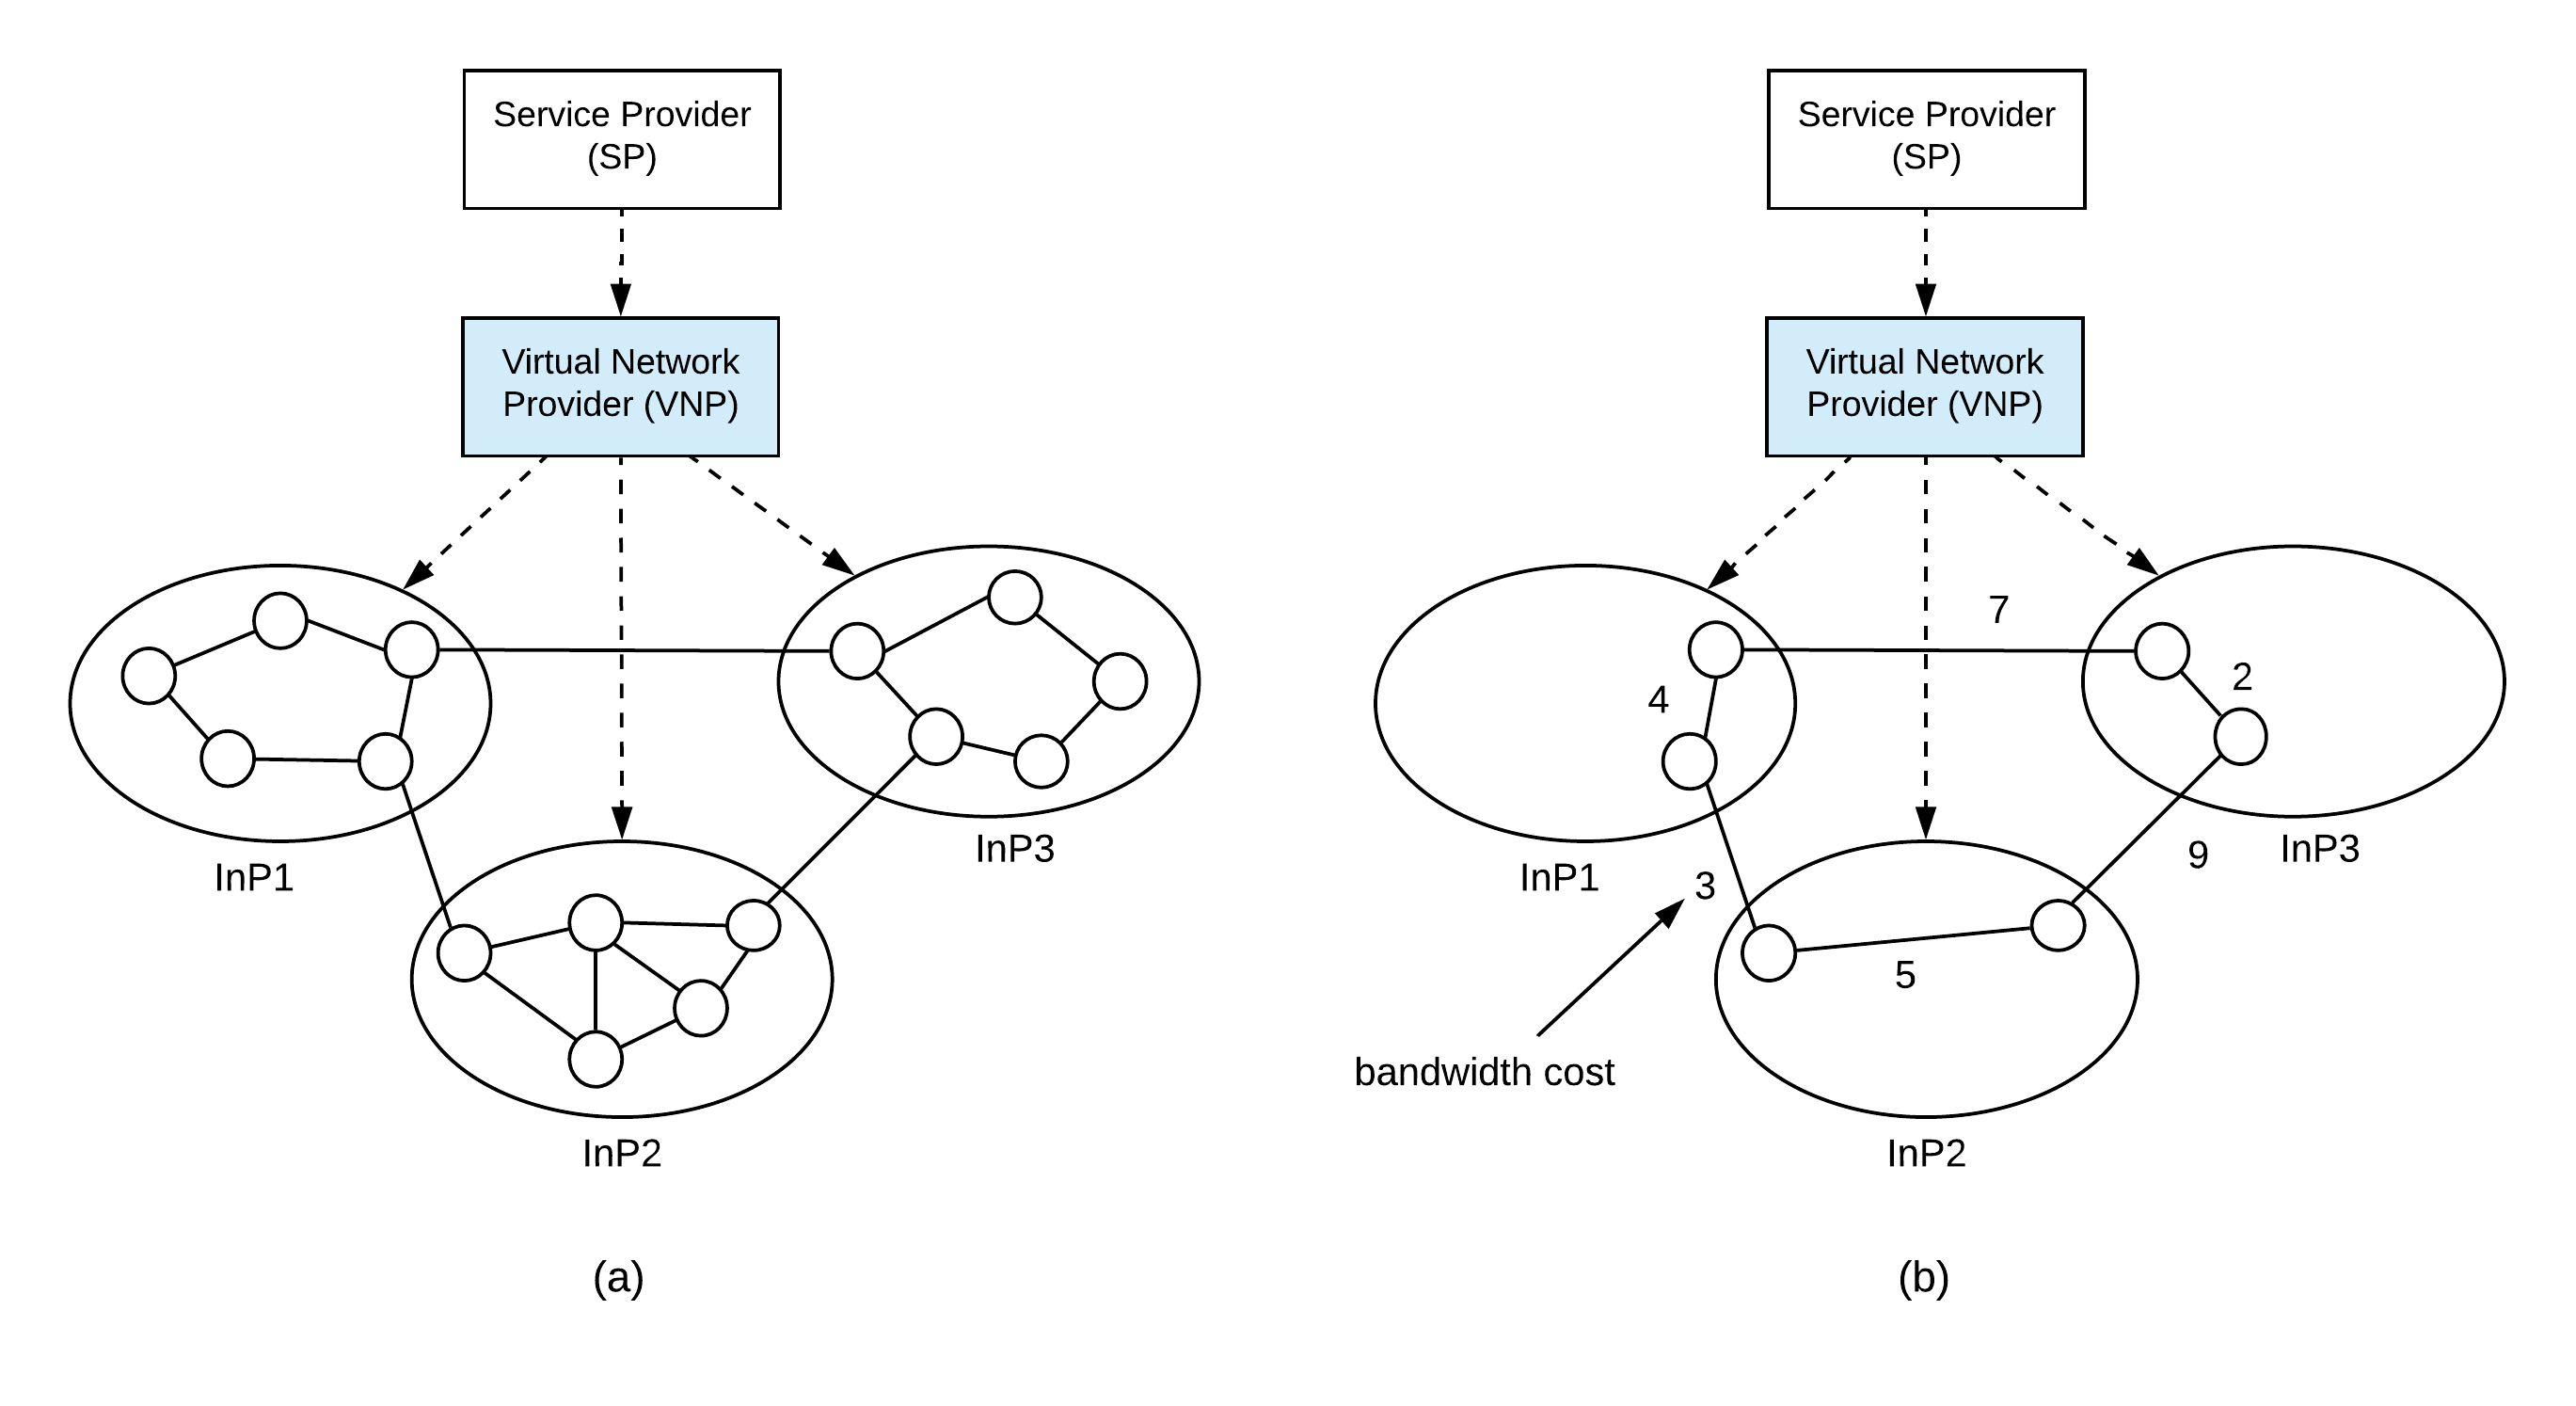
\includegraphics[width=0.48\linewidth]{gfx/multiprov}} \quad
	\subfloat[VNP's limited view on substrate network.]
	{\label{fig:multiprov_b}%
	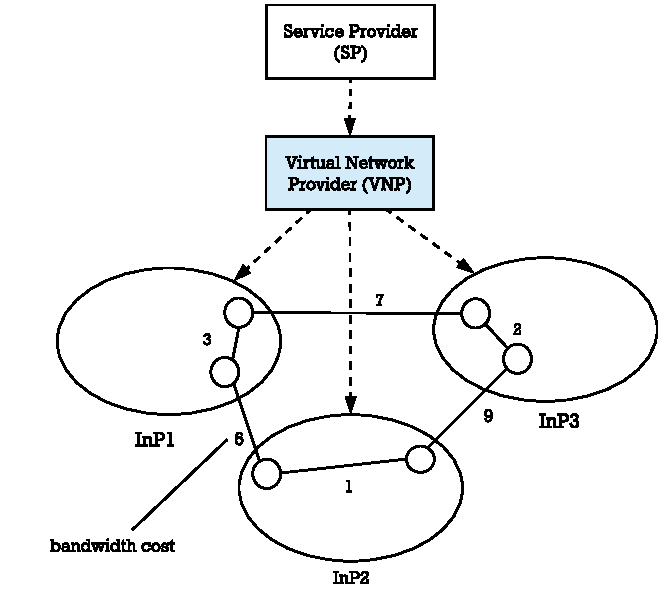
\includegraphics[width=0.48\linewidth]{gfx/multiprov2}} \\
	\caption{Virtual network Request across multiple InPs using a VN Provider. Adapted from \citep{dietrich2015multi}.}
	\label{fig:multiprov}
\end{figure}

Furthermore, in \citep{dietrich2015multi}, the slice embedding is achieved by subsequently perfoming the following tasks: Firstly, the above-mentioned resource information is sent from the InPs to the VNP, who stores it. Secondly, the VNP matches the service provider request with this collected data. Thirdly, the corresponding partitioning and mapping algorithms are applied (not discussed in this thesis). 

In addition, the results of this research prove that the centralized VNE approach provides embedding costs not much higher than in an ideal case scenario (InPs announcing all required information) and a high ratio between the number of slices requested and later allocated. Despite the positive findings, this scenario suffers mainly from scalability, since everything relies on a single centralized authority: the virtual network provider. In addition, it assumes that InPs will be constantly advertising their updated data to the VNP, which can lead to undesired costs.

Therefore, other approaches where the actors benefit from a more scalable and distributed slice embedding need to be further investigated.

\subsubsection{Distributed Slice Embedding}

Many existing solutions \citep{houidi2011virtual}, \citep{dietrich2015multi}, \citep{dietrich2017multi} rely on a centralized party (VNP) that stores the InPs disclosed information and then performs the partition of the virtual network request. 

However, if the SPs and InPs are not willing to trust a centralized broker, this central actor could be removed, which provides a direct communication and a better system scalability. Distributed network slice embedding has already been investigated in:

\begin{itemize}
	\item In \citep{esposito2013general}, a \textbf{consensus-based auction for distributed slice embedding (CAD)} is proposed. In particular, the physical nodes, which are owned by a single or different InPs, bid on virtual nodes. This value is subsequently stored in a vector $b_i$, where $i$ is the physical node. Afterwards, once the bidding phase concludes, each physical node exchange the bids with its neighbors to reach an agreement for the auctioned virtual nodes. This bidding can be for a single slice (2 virtual nodes and 1 link) or for the entire slice (multiple virtual nodes and links). In the former, there is a limit on the number of biddable nodes, which produces multiple iterations (excessive time). Despite in a multi-provider VNE scenario, the latter is more suitable, the InPs willingness to disclose their internal information will hamper the performance. Hence, this approach provides better scalability (decentralization), but it is not proper for our scenario since it does not solve our LID problem.
	\item In \citep{chowdhury2010polyvine}, a \textbf{policy-based inter-domain VNE framework (PolyViNE)} is presented. In PolyViNE, each InP embeds part of the VN request, while they cooperate with other InPs in a decentralized manner. In addition, forwarded decisions are location-based. For instance, in Figure \ref{fig:multi} each virtual node $\{A,B,C,D\}$, has a prefered geolocation. Afterwards, the matched InPs receive a notification for embedding the specific virtual node (e.g. InP3 with virtual node D). This process starts with the SP sending its VN request to multiple trusted InPs who reply back with the corresponding embedding and its prices (bidding). Then, the SP will choose the most economical embedding. However, to ensure performance each SP needs to know $k^{SP} \geq 1$ InPs and each InP $k^{InP} \geq 1$ InPs. In addition, if the VN is not completely mappable by a single InP, the InP embeds its part and forwards the other to a known InP. Despite, PolyViNE introduces a decentralized approach handling LID and uses the interesting location-assisted embedding, it has some drawbacks that need to be covered. Firstly, each InP has an extra overhead in communicating the rest of the VNR when this is not fully mapped. Secondly, the bidding to provide a competitive market is a great solution, however, the bids can be publicly known by other InPs. Thus, a better bidding process preventing InPs from revealing its confidential data is required. Finally, the condition that SPs and InPs need to know at least 1 InPs can lead to an application poor performance.
	
\begin{figure}[bth]
	\centering
	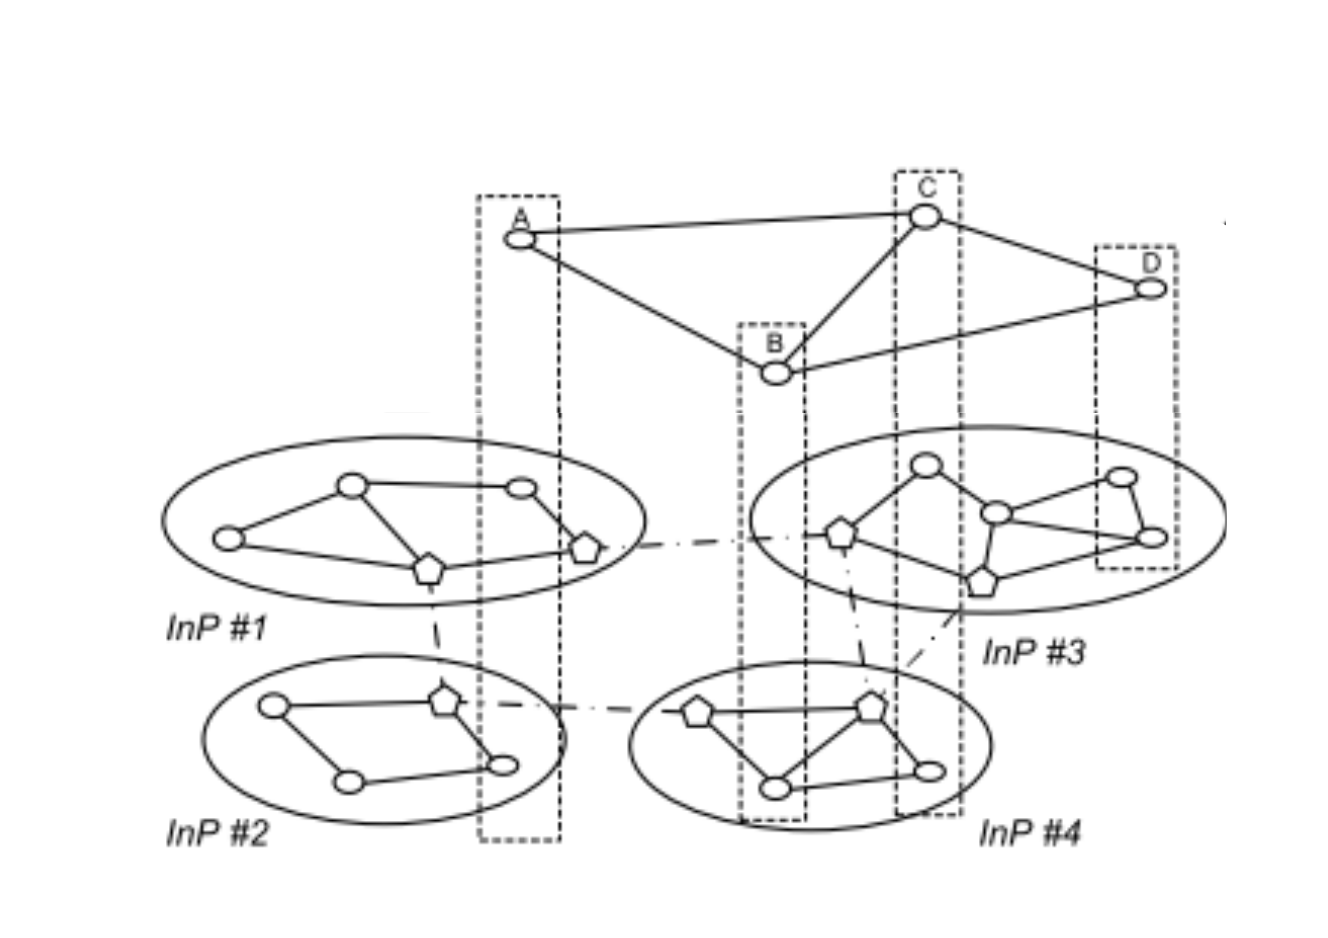
\includegraphics[width=0.5\linewidth]{gfx/multi}    
  	\caption{Multi-provider virtual network embedding \citep{chowdhury2010polyvine}.}
  	\label{fig:multi}
\end{figure}

\item Finally, in \citep{zaheer2010multi}, an \textbf{automated service negotiation framework (V-Mart)} is implemented. The V-Mart is also decentralized and based on an auction mechanism, the Vickrey auction model.
Though this approach ensures a fair market, thanks to the Vickrey auction model, it does not guarantee performance. The reason is that the VNE process deployed is a second-stage auction where explicitly all the InPs need to interact during the VN embedding. Thus, the VNE results in a high-demanding task. In addition, the sealed-bid is proposed to be done by a trusted 3rd party, which could cause again confidence issues. Nevertheless, the main V-Mart shortcoming is that it does not solve the LID problem, since it does not enforce inter-domain policies.

\end{itemize}

\section{Analysis of Related Work} \label{analysisOfRelatedWork}

Through relevant examples in supply chain management, as the presented in section \ref{manufacturing}, we can observe the blockchain's potential mainly in areas, where entities are willing to exchange data without trusting a third party. Despite the research does not include detailed specifications, such as the blockchain's type or mining strategy, a useful system design has been provided. In addition, some of the main benefits compared to centralized technologies are contemplated:

\begin{itemize}
	\item \textbf{Disintermediation:} Thanks to the consensus mechanisms, blockchain runs without a central administrator. Thus, intermediaries are not required for realizing transactions which suppresses all the significant costs of involving middle-parties \citep{mainelli2015sharing}. For instance, in the presented example, users were able to transfer ownership, just signing the product's contract.
	\item \textbf{Data management and redundancy:} Blockchain helps us in coordinating, validating and storing the distributed data in a decentralized manner. It also provides automatically redundancy since users own the same data. Reversely, in centralized systems, the users need to explicitly create a backup of the databases, for preventing the loss of data if the system crashes.
	\item \textbf{Unconstrained technology:} As actors can define and establish their own rules (smart contracts), new business models open up.
	\item \textbf{Privacy:} Thanks to cryptography, users can interact with untrusted partners. For example, in the alredy mentioned example, all actors were able to coordinate its services through the PLM process, which before would have been a complex task as they do not trust each other.
    \item \textbf{Transparency and integrity:} All the changes that are made to the contract data are directly visible to the other users. In addition, once a transaction is executed, its immutable since it cannot be altered or deleted.
	
\end{itemize}

\begin{table}[bth]
	\myfloatalign \footnotesize
	%18 columns
	\begin{tabularx}{\textwidth}{>{\raggedright\arraybackslash}p{3.5cm} >{\raggedright\arraybackslash}p{1cm}p{0.65cm}p{0.65cm}p{0.65cm}p{0.65cm}p{0.65cm}p{0.65cm}p{0.65cm}p{0.65cm}p{0.65cm}p{0.65cm}p{0.65cm}}
	\textbf{Approach} & \textbf{System} & \rot{\textbf{Scalability}}  & \rot{\textbf{Trusted third party (TTP)}} & \rot{\textbf{Sealed bidding}} & \rot{\textbf{Bid exchange between InPs}} & \rot{\textbf{LID problem solved}} & \rot{\textbf{Location-assisted VNE}} & \rot{\textbf{User notified}} & \rot{\textbf{S-performance}} & \rot{\textbf{L-performance}} & \rot{\textbf{Low VNE cost}} & \rot{\textbf{Low cost (\euro)}}\\ 
		\hline
		Multi-provider VNE framework with VNP \citep{dietrich2015multi} & C & \xmark & \cmark & \xmark & \xmark & \cmark & \cmark & \xmark & \cmark & \xmark & \cmark & \xmark \\ \hline
		CAD - Consensus-based auction for distributed slice embedding \citep{esposito2013general}   &  D & \cmark & \xmark & \xmark & \cmark &  \xmark & \xmark & \xmark & \xmark & \cmark & \xmark & \cmark \\ \hline
		PolyViNE - Policy-based inter-domain VN embedding framework \citep{chowdhury2010polyvine}   &  D & \cmark & \xmark & \xmark & \cmark &  \cmark & \cmark & \cmark & \xmark & \cmark & \cmark & \cmark \\ \hline
		V-mart - Automated service negotiation framework \citep{zaheer2010multi}   &  D & \cmark & * & \cmark & \xmark & \xmark & \xmark & \cmark & \xmark & \xmark & \xmark & \xmark \\
		\hline
	\end{tabularx}
		\caption{Comparison of virtual network embedding approaches - Overview for system features implemented as \textit{yes} (\cmark), \textit{no} (\xmark), \textit{to some extent} (*). Abbreviations: \textit{D} = decentralized, \textit{C} = centralized, \textit{L-performance} = large scenario performance and \textit{S-performance} = small scenario performance.}
	\label{tab:Comparison}
\end{table}

On the other hand, in the second part of this chapter, we have investigated related work on multi-provider VNE suffering from LID. A comparison for each of the approaches presented before is shown in Table \ref{tab:Comparison}.

First of all, we can observe that decentralized systems provide obviously a better scalability because the application does not rely on a single point of failure. In centralized systems, this central entity has to be trusted since it stores and manages all the information. In contrast, all the presented related work on decentralized VNE, uses a bidding mechanism to reach an agreement between the SPs and InPs.

Despite being a decentralized system, \cite{zaheer2010multi} uses to some extent a trusted third party (TTP). This is because, it is the only approach offering a sealed-bidding between users, although with the use of a trusted third party. We also notice that in \cite{esposito2013general}, \cite{chowdhury2010polyvine} the bids are exchanged between InPs to cooperate in the VN embedding, which results in undesired computational costs. In contrast, centralized systems \citep{dietrich2015multi}, perform the service negotiation without using auctions, since they trust a middle-party managing these operations.

Moreover, one of the main challenges is to solve the limited information disclosure issues. We notice that \citep{dietrich2015multi}, \citep{chowdhury2010polyvine} deal with the problem, accessing public information not considered confidential and performing the VNE under its internal policies respectively. In addition, they provide location-assisted VNE, which facilitate the VN request partitioning across different InPs. The last, it also introduces a notification system, where the InPs gets notified upon VN request, which avoids time spending in request synchronization. 

In general, centralized systems provide a better throughout in small scenarios since all the information is managed by a central entity. Hence, data sharing or user's cooperation is not needed before performing any operation. Conversely, decentralized systems benefit from large scenarios. Firstly, because the more users participating in an auction, the more competitive the market is. Secondly, all the activities are diversified, and thus, the decision-making is more efficient. 

Finally, we classified costs into virtual network embedding and economic. Overall, we observe that VNE costs are lower when using a centralized system \citep{dietrich2015multi}, although when the parties are efficiently coordinated in a decentralized scenario, the costs are also extremely reduced \citep{chowdhury2010polyvine}. 

Regarding economic costs, they are obviously higher for centralized systems, as the application performance depends only on a central entity, which needs to be financed for their computational and maintaining costs.



\section{Summary}

After comparing the different multi-provider VNE approaches exposed throughout this chapter, we ascertain that each of them introduces innovate features to handle network virtualization. However, there is no single solution that satisfies at the same time the following requirements:

\begin{itemize}
	\item Scalability.
	\item LID problem approached with data confidentiality.
	\item Large scenario performance.
	\item Low computational and economic costs.
\end{itemize}

Therefore, the main focus of this thesis will be to investigate and later implement an approach that gets rid of the VNP, and which fulfills the above-mentioned virtual network embedding demands. Here, we foresee that blockchain could play a significant role.


%*****************************************
\chapter{Design}
\label{ch:design}
%*****************************************

Based on the challenges highlighted in the previous chapter, a conceptional design of a multi-provider virtual network embedding approach using blockchain is now introduced. First, we define the requirements and assumptions used for the design process. Afterwards, we present the fundamental goals expected from the system, followed by a general overview of the architecture along with its functionality. In addition, important features for our application will be discussed, in particular, the blockchain type, the mining strategy, the authentication system and the auction model used.

\section{Requirements and Assumptions} \label{requirements}

Since blockchain is a disruptive technology, apparently it seems that it could improve many existing systems. However, is the blockchain the only technology to approach scalability, security or data handling between organizations? Why not to use a traditional database rather than a blockchain? The truth is that there is not a single solution or better technology than the others, as it depends on user's requirements. Thus, it is important to understand in which scenarios the blockchain could replace existing infrastructures. For this purpose, in Figure \ref{fig:bcFlowchart} we present a flowchart \citep{wust2017you}, which pretends to guide users in determining whether blockchain is the appropriate solution to resolve their problems, and if yes, the suitable BC type. We will also follow the diagram to decide if our defined VNE scenario demands match the blockchain use case.

\begin{figure}[bth]
	\centering
	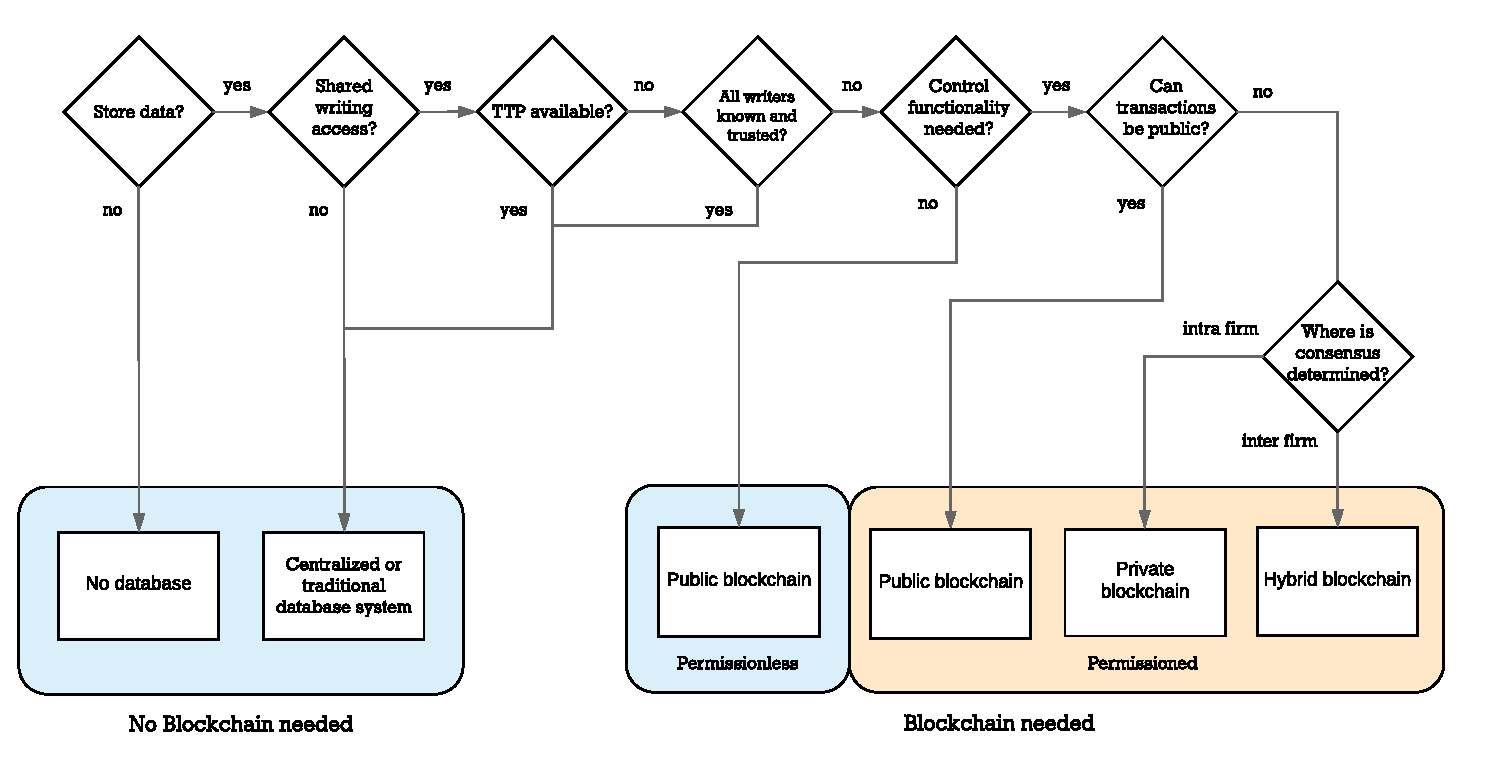
\includegraphics[width=1\linewidth]{gfx/bcFlowchart}    
  	\caption{Flowchart to determine whether blockchain is the suitable solution. Adapted from \citep{wust2017you}.}
  	\label{fig:bcFlowchart}
\end{figure}

Before starting to analyze the flowchart, one statement needs to be clarified: if the user does not need to store data, no blockchain or database is required. The discussion arises when multiple writers are willing to exchange data without relying on a trusted third party (TTP). In this context, a writer is a user that performs the four basic functions of persistent storage: create, read, update and delete data (CRUD). If they trust a TTP, a traditional or centralized database will always provide a better throughput. However, if this is not the case, then the user should first consider if all the writers are known and trusted. If so, again a typical database (e.g. SQL) will be better positioned. If all the last requirements are satisfied, or in other words, multiple untrusted writers are willing to update the state of a system without trusting a middle actor, it is then that the blockchain is a reasonable solution.

In Figure \ref{fig:bcFlowchart}, we also classify blockchains into two groups: \textit{permissionless} and \textit{permissioned} blockchains. To decide between these two approaches, the user should consider if he is willing to control his customized blockchain, creating his own specifications. For example, the main networks of Bitcoin and Ethereum are permissionless, where users are added to the network and thus, restricted to its policies. In Table \ref{tab:blockchainTypes} the main characteristics of each blockchain type are summarized. Scalability is an important topic in the blockchain domain, where we distinguish: node scalability and performance scalability. The former is the capacity to add new participants in the blockchain without losing performance, and the latter is the number of transactions executed per second. In addition, note that some features depend on the blockchain design decisions since permissioned blockchains capabilities are easily modifiable. For example, if consensus algorithms are used, the interaction between users should have a cost in order to ensure performance, i.e miners need to be rewarded with transaction fees.

\begin{table}[bth]
	\myfloatalign \footnotesize
	%18 columns
	\begin{tabularx}{\textwidth}{>{\raggedright\arraybackslash}p{4cm} >{\raggedright\arraybackslash}p{6cm}>{\raggedright\arraybackslash}p{6cm}}
	\textbf{Features} & \textbf{Permissionless} & \textbf{Permissioned}\\ 
		\hline
		Type & Public & Public, private and hybrid blockchain \\
		Control functionality/ Transaction processing & Fully decentralized & One or a small group of pre-selected entities \\
		Access control & Open access & Authorized access \\ 
		Number of users & High & Low \\
		Number of untrusted users & High & Low \\
		Writers & Any user participating & Permissioned group of people, e.g. bank customers\\
		Centrally managed & No & (*) \\
		Security & Consensus algorithms (e.g PoW) & (*) \\
		Transaction fee & Yes & No (*) \\
		Trusted & No & Yes \\
		Node scalability & High & Low \\
		Performance scalability & Low & High \\
		Use cases & Cryptocurrencies (e.g. Bitcoin \citep{bitcoin}) & Transactions in business networks (Hyperledger Fabric \citep{hyperledger}) \\ \hline
	\end{tabularx}
		\caption{Types of blockchain: permissionless vs permissioned. Adapted from \citep{wust2017you}. (*) depending on blockchain design decisions.}
	\label{tab:blockchainTypes}
\end{table}

Furthermore, as stated in Figure \ref{fig:bcFlowchart}, permissioned blockchains are divided into:

\begin{itemize}
	\item \textbf{Public permissioned blockchain:} Decentralized, all the users are allowed to read the system's state (transactions can be publicly verified), although only some of them have writing privileges.
	\item \textbf{Private blockchain:} Centralized, with access and writing permissions restricted to a set of users. Note that in the flowchart (Figure \ref{fig:bcFlowchart}) this corresponds to an intra-firm consensus since it is only managed by a single organization. We understand by firm a traditional company or a pre-selected group of users.
	\item \textbf{Hybrid/Consortium blockchain:} Partly decentralized. The blockchain is controlled by a pre-established set of entities (inter-firm). In this model, each of these firms coordinates and ensures the system's functionality. Note that compared to the private blockchain, multiple firms maintain and serve the infrastructure rather than a single one. Thus, a consensus between these parties is also needed. For example, currently, several banks deploy common blockchains to manage their shared data and reduce intermediaries costs. In this case, each bank will control a node, resulting in a better throughput in terms of scalability.
\end{itemize}

After presenting the blockchain use cases and types, we observe some similarities between a traditional shared database and a permissioned private chain, since they are both managed by a group of users, which simultaneously maintain the same confidential data. Despite private blockchains could be seen only as another term used to name shared databases, the truth is that each technology has its trade-offs, without mentioning scalability or cost issues. On one hand, centralized databases will always have better throughputs since, in addition to the basic transaction operations, blockchains need to perform cryptographic verifications, and ensure a consensus between the other participating nodes. On the other hand, private blockchains are less prone to malicious attacks, inasmuch as they spend a longer period in checking errors or validating transactions, than regular databases. The blockchain also organizes data into blocks, which are appended once new data arrives. Therefore, as already noted, if users trust each other and a high-performance is desired, using a blockchain is not a suitable solution.

\subsection{Virtual Network Embedding with LID scenario}

In section \ref{analysisOfRelatedWork}, we have concluded that although plenty of work in network virtualization has been conducted, to the best of our knowledge, there is still no approach under LID that gets rid of the broker (VNP), providing scalability, confidentiality, and low-cost performance. Thus, after having spotted the main benefits of integrating blockchain in real-scenarios, among which disintermediation, privacy and transparency need to be highlighted, we assume that this technology could improve the VNE business process. Nevertheless, first, we should investigate whether our scenario could be integrated with a blockchain.

In network virtualization, we mainly encounter users with two different roles: Infrastructure Providers and Service Providers. Moreover, as the VNE is typically performed by the same parties across the countries, e.g. Deutsche Telekom, Vodafone or O2 in Germany, the scenario is restricted to a limited amount of users that barely changes. Therefore, we are facing an application where multiple known users that probably do not fully trust each other, want to reach a virtual network agreement, without relying on a third party. The decision of not including a TTP or VNP is mainly to avoid exchanging the InPs internal network cost models to an intermediate actor.

Observing the last mentioned requirements, we foresee that blockchain could be a suitable solution for our VNE scenario suffering from LID. However, an appropriate blockchain type still needs to be chosen. Obviously, the service negotiation between InPs and SPs is performed in a private environment, which automatically removes the permissionless and permissioned public blockchain options. Hence, the decision should be taken between a private or a hybrid blockchain.

One of the main requirements noticed from the previous related work is that our approach should address scalability issues. Accordingly, using a private blockchain, which is a centralized system managed by a single firm, will provoke that users rely again on a central point or trusted party, converting it to an unfeasible solution. Thereby, the \textbf{partly decentralized hybrid blockchain} seems to be the most suitable solution. In this scenario, a firm corresponds to each interested InP or SP willing to possess and control a blockchain node, in order to ensure the network virtualization functionality.


\subsection{Smart Contracts and Ethereum} \label{smartContractsAndEthereum}

After having spotted the most suitable blockchain type for our VNE environment, the non-trivial decision of selecting a blockchain platform needs to be taken. Prior to this, we need to consider whether our scenario could profit from the potential of smart contracts. Despite in subsection \ref{smartContracts}, it has been discussed what smart contracts are, it is also required to notice when they can be used. Thereupon, a market study regarding smart contracts and its application fields will not be conducted due to its extended dimension. Nonetheless, we enumerate the main usage examples of smart contracts in business to business processes \citep{blockchainBerkeley}:

\begin{itemize}
	\item \textbf{Settlement agreement:} Since smart contracts can be personalized, it enables that participants reach any kind of agreement without involving third-parties costs.
	\item \textbf{Frequently executed tasks:} Users regularly performing the same operations, can accelerate processes by depicting them on a smart contract code.
	\item \textbf{Self-operating databases:} Thanks to the blockchain, secured shared databases with low-costs are easily deployed. In addition, smart contracts can automate the interaction with this stored data, providing speed, real-time transparency and at the same time, opening new business models. 
\end{itemize}

In the presented network virtualization example, as the users negotiate the lease of virtual nodes over and over to reach an agreement, this task could be perfectly reflected in a contract code. Apart from handling smart contracts, the blockchain platform chosen needs to fulfill the following prerequisites \citep{macdonald2017}: 

\begin{itemize}
    \item \textbf{Easy to build, use and learn:} A low effort in setting the platform is essential. Thus, the smart contracts should be written or derived from common languages in the programming world, such as JavaScript or Python.
    \item \textbf{Support and documentation:} A consolidated platform, which is not in its early stages and with a high-maturity level achieved, is extremely needed. An active community of developers behind the project is also fundamental, e.g. with a considerable number of Github stars and forks.
    \item \textbf{Blockhain type:} Though it could be desirable that the main network is permissioned and hybrid or private, currently, in open source code platforms, the blockchain types can be modified. Thus, it is not a must-have feature that the predefined main network type matches the desired one.
\end{itemize}

\begin{table}[bth]
	\myfloatalign \footnotesize
	%18 columns
	\begin{tabularx}{\textwidth}{>{\raggedright\arraybackslash}p{2.5cm}>{\raggedright\arraybackslash}p{2.5cm}>{\raggedright\arraybackslash}p{2.5cm}>{\raggedright\arraybackslash}p{2.5cm}>{\raggedright\arraybackslash}p{2.5cm}>{\raggedright\arraybackslash}p{2.5cm}}
		\textbf{Characteristics} & \textbf{Bitcoin} & \textbf{Ripple} & \textbf{Ethereum} & \textbf{Hyperledger Fabric} & \textbf{R3 Corda}\\ 
		\hline
		\textbf{Application} & Payments & Payments & General purpose & General purpose & Financial services \\
		\textbf{Governance} & Bitcoin developers & Ripple Labs & Ethereum developers & Linux Foundation & R3 \\
		\textbf{Main network} & Permissionless, public & Permissioned, public & Permissionless, public and private & Permissioned, private and hybrid & Permissioned, private and hybrid \\
		\textbf{Data model} & UTXO-based & UTXO-based & Account-based & Account-based & UTXO-based \\
		\textbf{Configuration effort} & Low & Low & Low & High & High \\
		\textbf{Support and Documentation} & High & Medium & High & Medium & Low \\
		\textbf{Smart contract language} & - & - & Solidity (JS), Serpent (Python) and LLL & Go, Java & Kotlin, Java \\
		\textbf{Currency} & BTC & XRP & ETH & None & None \\
	\hline
	\end{tabularx}
		\caption{Comparison of different blockchains platforms. UTXO stands for Unspent Transaction Outputs.}
	\label{tab:blockchainComparison}
\end{table}

In Table \ref{tab:blockchainComparison}, a comparison of the most common blockchain platforms, in our opinion, is depicted. Since in our application, a scripting language with smart contracts is preferable and Bitcoin and Ripple by default do not incorporate them, these platforms are automatically discarded. On the other hand, Hyperledger Fabric and R3 Corda are popular used platforms, whose main network perfectly fits our requirements. However, they provide customized blockchains with a high configuration effort, where its specifications need to be carefully designed. Thus, Ethereum seems to be the better positioned as a platform with a straightforward setup and usage is required.

Ethereum is a mature and easy to build project based on smart contracts with a large number of developers behind, who are actively discussing and improving its functionality. Thanks to this, the creation of new business models is extremely facilitated for newcomers. Furthermore, Ethereum smart contracts are written in Solidity and Serpent, which are similar to JavaScript and Python respectively. Despite the fact that Ethereum's main network (public permissionless) is not the ideal for our scenario (permissioned and hybrid), the simple and easy set up of the platform's environment, allow us to quickly deal with these issues. Finally, the Ethereum Virtual Machine (EVM) is a Turing-complete system, which helps us in obtaining the maximum benefit from the smart contract's potential.

Overall, thanks to the blockchain, more precisely Ethereum and smart contracts, the VNP could be replaced with a secure, flexible and coordinated system. In this scenario, the reliance is now distributed among multiple blockchain nodes rather than just on a costly single entity. However, the block generation time or the service negotiation performance, are examples of challenges that need to be thoroughly investigated along the thesis.

\section{System Design}

Based on the requirements and assumptions defined in the previous section, the design of a multi-provider virtual network embedding system using the blockchain technology is presented. At first, the fundamental goals that are expected from the system are defined, followed by a general overview of the architecture and its design features.

\subsection{Fundamental Goals}

In general, the fundamental goals for network virtualization relies on simulating baremetal networks, providing improvements in terms of flexibility, manageability, and costs. In this scenario, the SPs are willing to embed virtual nodes across different InPs to create customized virtual networks. This embedding task consists first of the VN request partitioning and later, of the corresponding mapping to the InP's physical nodes, such that virtual node and link requirements are fulfilled. However, the problem becomes clear when InPs are not willing to disclose detailed information about their resource availability or network topologies, which is indispensable for the VN partitioning efficiency \citep{dietrich2015multi}. In this thesis, the VN partitioning is treated as a cost minimization problem, where the service provider pursues the minimum VN embedding cost\footnote{From now on, we use the term cost to refer the value that the SP must pay for embedding the virtual nodes across the InPs. This value is derived from the InP bids.}. In a real world, there are more parameters that could be taken into consideration, such as the quality of the service.

In a multi-provider scenario with full information disclosure (Figure \ref{fig:problem_a}), the VN request partitioning is efficiently computed since the infrastructure provider's internal information is publicly available. Conversely, the lack of data in a limited information disclosure scenario (Figure \ref{fig:problem_b}), directly affects the VNE throughput. Nevertheless, there is some information not considered confidential by the InPs, such as the location or the virtual node types offered by the peering nodes. For instance, in Figure \ref{fig:problem}.b, the InP1 has two peering nodes with locations in Germany and Switzerland, and virtual node types $\{A, B, D, E\}$ and $\{F, G\}$ respectively. These virtual node types, as Amazon EC2 \citep{amazonEC2} does, are used to classify the resources in different groups, each having common attributes, such as CPU, memory, storage and network capacity. Thus, in this thesis, new embedding strategies and approaches to facilitate the service negotiation process between the InPs and SPs will be developed.

Moreover, in section \ref{analysisOfRelatedWork}, we have contemplated that decentralized approaches tend to use auctions to negotiate the network workflows. Regardless of the auction model applied for our VNE framework, there are several metrics that need be considered: 

\begin{itemize}
    \item \textbf{Efficient:} The virtual network embedding must be efficient in terms of synchronization, communication, and data sharing between the participating users.
    \item \textbf{Equality:} All participants, namely service providers and infrastructure providers, must have the same role's privileges. In other words, all SPs must be able to request the same amount of virtual networks over time and InPs bids must be treated equally in the application.
    \item \textbf{Market fairness:} The auction model requires that the SPs find the desired service at the lowest price and that the InPs obtain the highest possible revenue for the offered service.
    \item \textbf{Data confidentiality:} At the moment of bidding, in order to not alter the auction progress, the bids should be kept in secret. Finally, the winners can be publicly known.
    \item \textbf{No trusted auctioneer:} Since confidentiality is required, a middle party or auctioneer should not be capable of managing the auction workflow and thus, accessing the private bidding values.
     \item \textbf{Automated:} The virtual network embedding process needs to be automated with a friendly and easy-to-use framework.
\end{itemize}

\begin{figure}[bth]
	\myfloatalign
	\subfloat[Full information disclosure (FID).]
	{\label{fig:problem_a}%
	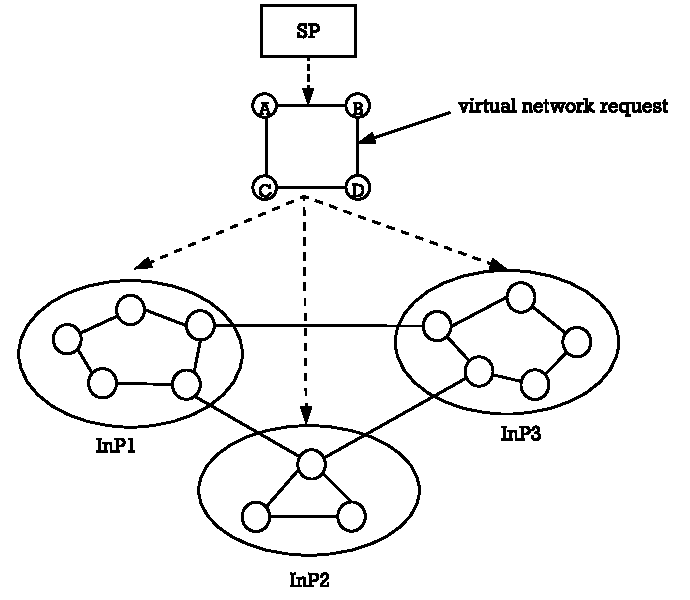
\includegraphics[width=0.48\linewidth]{gfx/Problem}} \quad
	\subfloat[Limited Information Disclosure (LID) with peering node locations and resource types.]
	{\label{fig:problem_b}%
	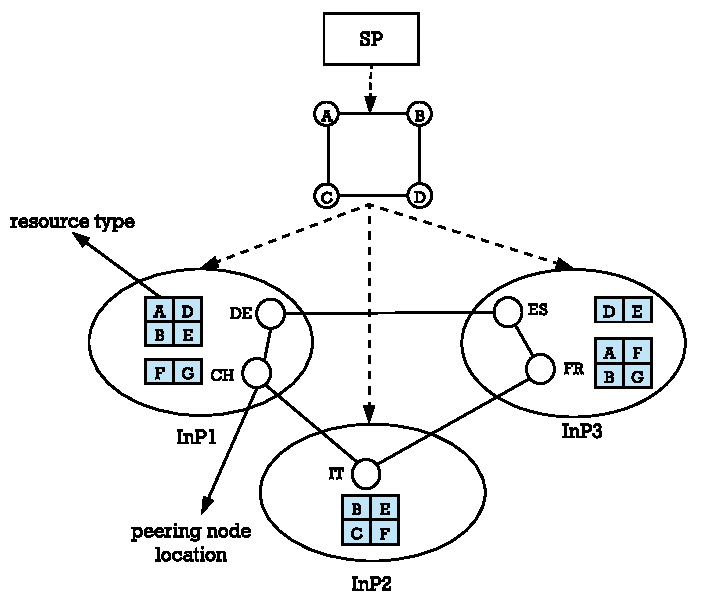
\includegraphics[width=0.48\linewidth]{gfx/Problem2}} \\
	\caption{Substrate network visibility. Adapted from \citep{dietrich2015multi}.}
	\label{fig:problem}
\end{figure}

\subsection{System Architecture}

\begin{figure}[bth]
	\centering
	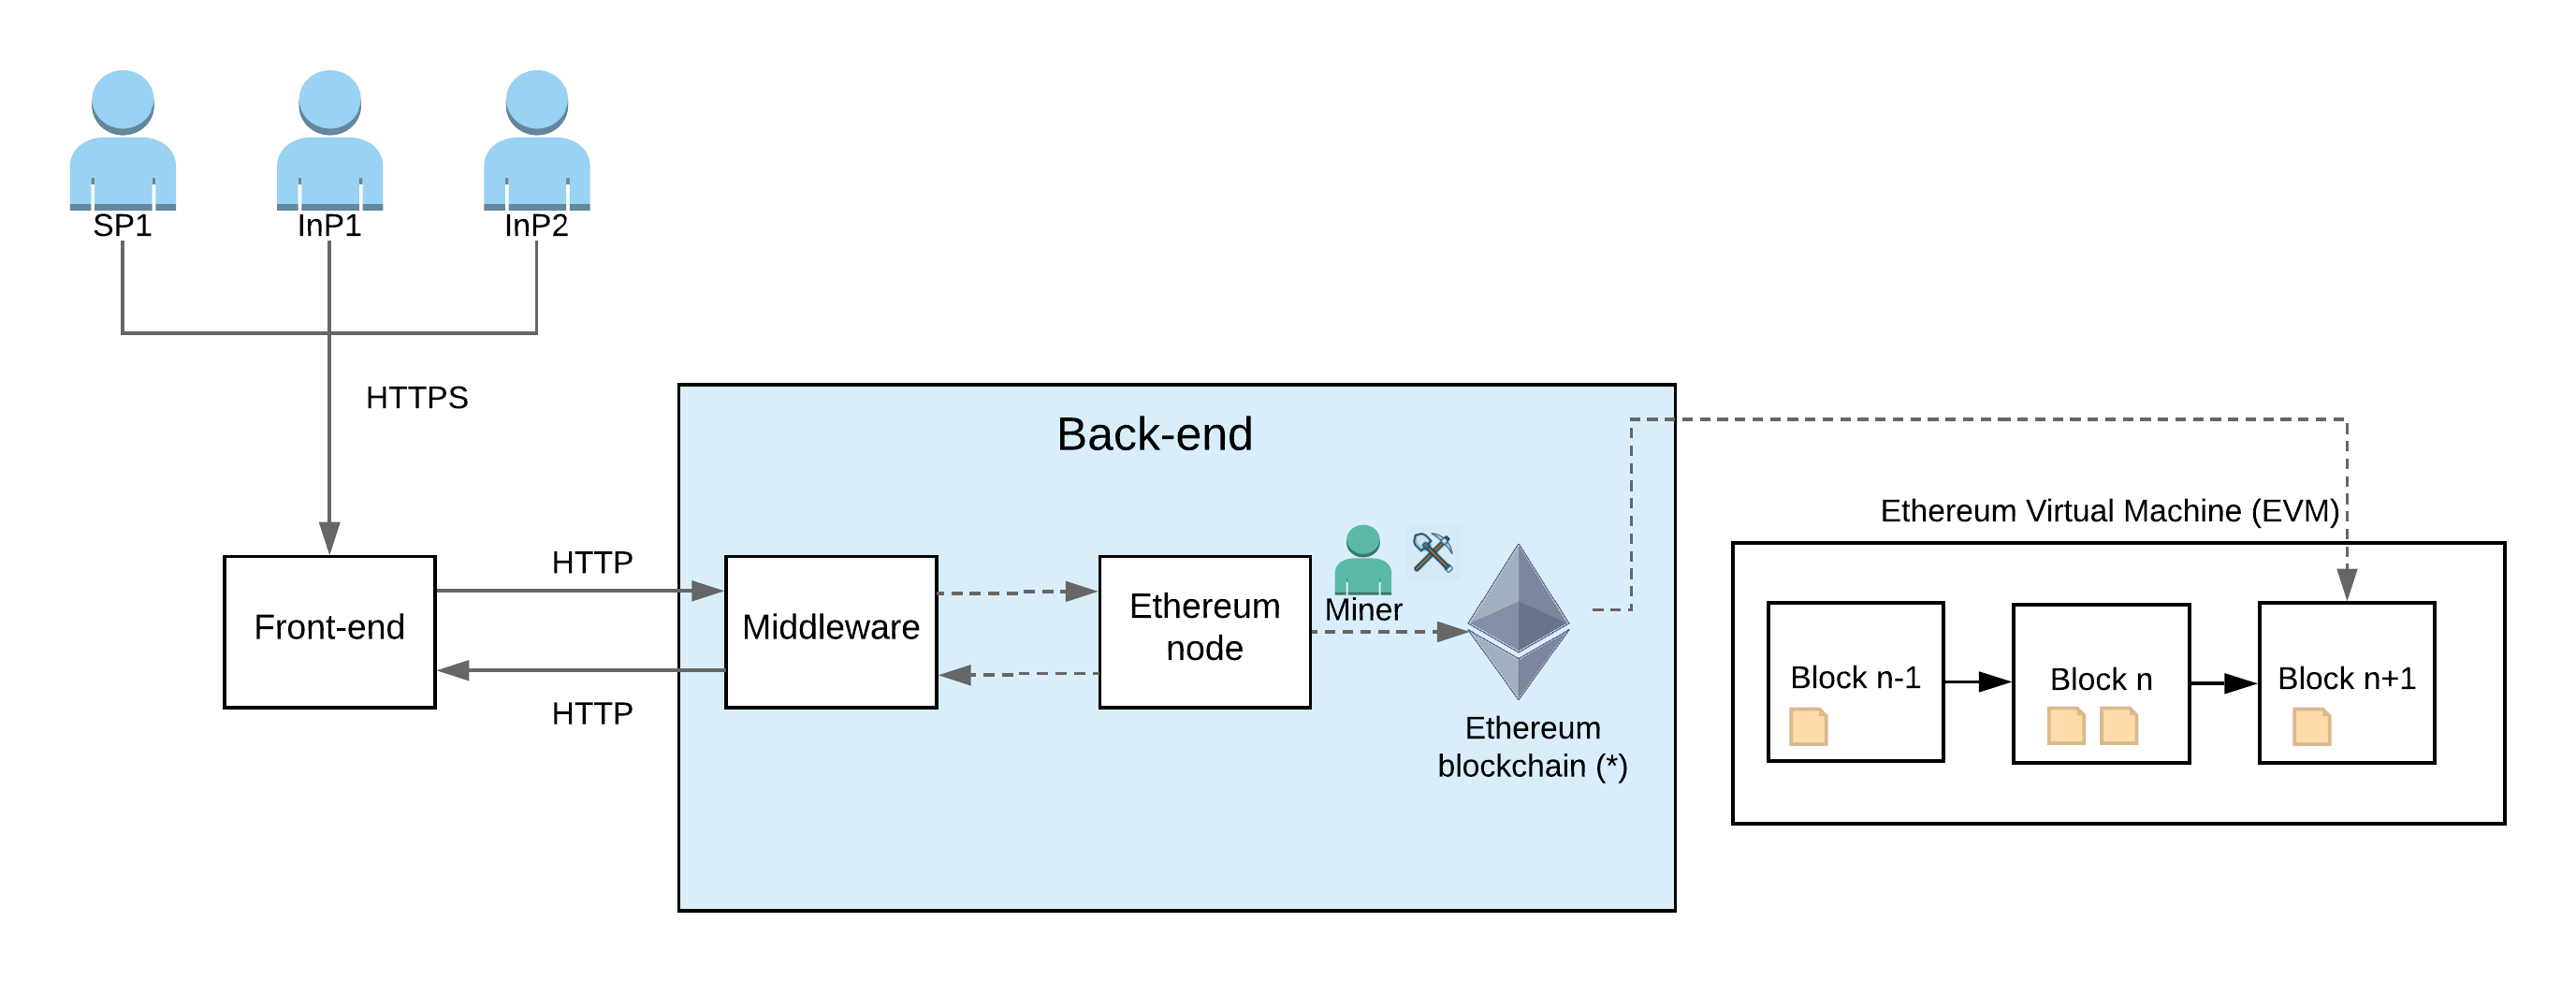
\includegraphics[width=1\linewidth]{gfx/designWorkflow}    
  	\caption{Our design for the system architecture. $u_i$ states for upper bound cost and $l_i$ for location.}
  	\label{fig:designWorkflow}
\end{figure}

After defining the main VNE problem that needs to be addressed, and describing the goals and metrics required for the design of our scenario, a system architecture is now presented, see Figure \ref{fig:designWorkflow}. Firstly, the proposed design shows the main components of the system, which are:

\begin{itemize}
    \item \textbf{Private group of users:} The system is composed of a private group, in which participants can be infrastructure providers or service providers. Since in private groups only certain members are allowed to access and alter the data, in this design, new users must ask for permission before joining the network. Furthermore, once entering the group, the newcomer can optionally act as a miner or just use the application without the need of maintaining a blockchain node.
	\item \textbf{User interface (UI):} Through an API (for automation), each member will efficiently interact with the blockchain application. Depending on the user's role, i.e infrastructure providers or service providers, the API will provide different functionalities. For instance, SPs have the ability to request virtual networks and InPs to bid for the proposed virtual nodes, but not the other way around. Thus, the available operations must be restricted to the user's privileges.
	\item \textbf{Ethereum blockchain:} One of the main differences between the Bitcoin and the Ethereum blockchain is that the first is transaction-based while the second account-based. For this reason, apart from a list of transactions, each Ethereum's block also stores the most recent state, i.e. the current account list with the corresponding balances. Nevertheless, every blockchain starts with the block 0, also called \textit{Genesis block}. Since it is the first block, it is the only one not pointing to a predecessor and it is typically hardcoded in a file called \textit{genesis.json}. This file contains some of the blockchain specifications, such as the difficulty or the gas limit. By modifying the value of these parameters, users are allowed to create blockchains based on their requirements. More details about the genesis file content used in our system will be discussed in chapter \ref{ch:implementation}.
	\item \textbf{Smart contracts:} Above, we have mentioned that each Ethereum block stores a list of accounts with their corresponding balances, among others. These accounts can be externally owned accounts (users) or contract accounts (smart contracts). In the case of smart contracts, they enable reflecting user's needs into code and can be created or called either from another contract or simply by an EOA. In our system, a static contract called \textit{Users} is contained, which will be permanently requestable. This contract will store all the participant's information, and whenever a new user registers, its state will be modified. In addition, this contract includes the InPs entered information about their substrate networks, such as the peering nodes or the substrate node types, which will be used to match the virtual network requests.
\end{itemize}

To provide a clearer view of the last mentioned components, the VNE functionality needs to be introduced. This VNE process entails the following steps (Figure \ref{fig:designWorkflow}):

\begin{enumerate}
    \item \textbf{VN request:} A service provider requests a virtual network, which can be represented in a graph as $G^{R} = (N^{R} , d^{R})$, where $N^{R}$ consists of a set of $k$ virtual nodes, and $d^{R}$ the set of all bandwidth demands between the virtual nodes $i,j \in N^{R}$. Here, the superscript $R$ stands for request. In addition, each virtual node $N_i \in N^{R}$ is formed by a collection of attributes, such as the desired location $l_{i}$ or the upper bound cost $u_{i}$, where the last term may be the maximum amount of money that the SP is willing to pay for virtual node $N_i$. Otherwise, if an upper bound cost for the whole network is specified $u_{G}$, the one for each virtual node will be treated as $u_{i} = \frac{u_{G}}{k}$.
    \item \textbf{Resource matching:} Before the auction starts, first, the associated set of attributes (e.g. location) of the requested virtual nodes $N^{R}$ are matched with the InPs entered data in the \textit{Users} contract. For instance, virtual nodes $\{A,B\}$ and $\{C,D\}$ will be matched with InPs possessing physical nodes in Germany (DE) and Switzerland (CH) respectively. In case no location $l_{i}$ is specified for the nodes $N^{R}$, the VN request will be broadcasted to all the registered infrastructure providers.
	\item \textbf{Auction start:} Using the previous information, the corresponding smart contract, i.e. a \textit{limited time auction}, is created. This contract contains: (i) the data related to the virtual network nodes and links, (ii) the address of the SP willing to lease virtual nodes, (iii) a list of all the InPs addresses matched, (iv) a lifetime and (v) a bidding period field. Since the bidding and the virtual network lifetime must terminate, in the first step, the SP must also add the bidding period and the lifetime fields to the request.
    \item \textbf{Notification and bidding period:} After the new auction contract is created, the included InPs, which are the only users with the ability to bid for the resources, are notified. This notification can be transmitted either by a push-based technology, where the server or publisher updates information on the client (e.g. Publish/Subscribe system) or by a pull-based technology, in which the client initiates the request of information from the server. In this thesis, our system utilizes a pull-based technology (section \ref{architecture}), such that the application is more customer-centric without the need of using and maintaining external databases apart from the blockchain. Since a pull-based system already fulfills the requirements, further approaches, such as creating complex contracts in the BC, are not considered in this thesis. Regarding the bidding, despite having a full view of the VN request and knowing the other matched InPs, each InP is only allowed to bid for their paired resources. For instance, InPs from Germany can only bid for the resources $\{A, B\}$. Before bidding, these users typically evaluate the request requirements into their substrate network, depicted as $G^{S} = (N^{S},  L^{S})$, such that $N^{S}$ and $L^{S}$ are the set of physical nodes and physical links respectively. Although InPs are interested in serving requests at maximum profit, a single InP can barely serve all the virtual nodes requirements. As a result, the virtual network just may be supplied by different infrastructure providers. More details about the bidding mechanism is presented in section \ref{vickrey}.
 	\item \textbf{VN request partitioning and mapping:} Once the auction has finished, each virtual node is assigned to the winning InPs so that the VN embedding cost is minimized. These winners are now publicly known by all the other participating users and thereupon, the service provider will contact them to ultimate the VN setting up, i.e. to perform the VN segment mapping.
\end{enumerate}

To summarize, the presented system design uses the blockchain technology, in particular, smart contracts, to enhance the VN partitioning efficiency in a multi-provider scenario with limited information disclosure. Nevertheless, up to now, this is only a conceptual design with a lot of features that must be further discussed.

\subsection{Blockchain Type and Mining Strategy}

The Ethereum's main network,  is public and permissionless, where all the users have access to the transferred values between accounts since value transfers cannot be blinded. However, since our described scenario has a small number of users, the fully public decentralized approach directly affects the application performance. Thus, as concluded in section \ref{requirements}, our focus is on \textbf{permissioned hybrid blockchains}, where a set of inter-firm entities control and maintain the blockchain functionality.

On the other hand, the default Ethereum's consensus algorithm will be used, which is at the time of writing, the \textbf{Proof-of-Work} protocol. Nevertheless, since the blockchain can be customized, in chapter \ref{ch:evaluation}, other mining strategies will be further investigated on their suitability.

In summary, although the Ethereum main network is public and permissionless, it can run as a private or hybrid blockchain, with the technology mechanisms and protocols remaining unaltered.

\subsection{Authentication System} \label{authenticationSystem}

In the following, we will discuss how a user is registered and authenticated to the system, see Figure \ref{fig:authenticationDesign}.

First of all, in order to deploy and use the presented design, a single or a group of InPs need to set up the environment. Afterwards, this consortium of InPs or a public authority, such as a regulatory agency, is responsible for inviting others users (InPs or SPs) to join his network, i.e. to create an Ethereum account (EOA) for the application. 

However, once these users are registered, the communication between them must be secured. For this reason, the blockchain technology applies the \textbf{public-key cryptography}, also called asymmetrical cryptography, which generates a public and private key pair. The first, as the name suggests, it is publicly disclosed, and the second must remain confidential to its respective owner. Since these keys are mathematically related, the information encrypted with a private key can only be decrypted with a public one, and vice-versa. In addition, the Ethereum address is derived from this key pair, more specifically, from the last 160 bits of the \textit{SHA3-256} hash of the public key. Thus, once a user creates a new Ethereum account, the blockchain generates a public and private key pair for this user.

\begin{figure}[bth]
	\centering
	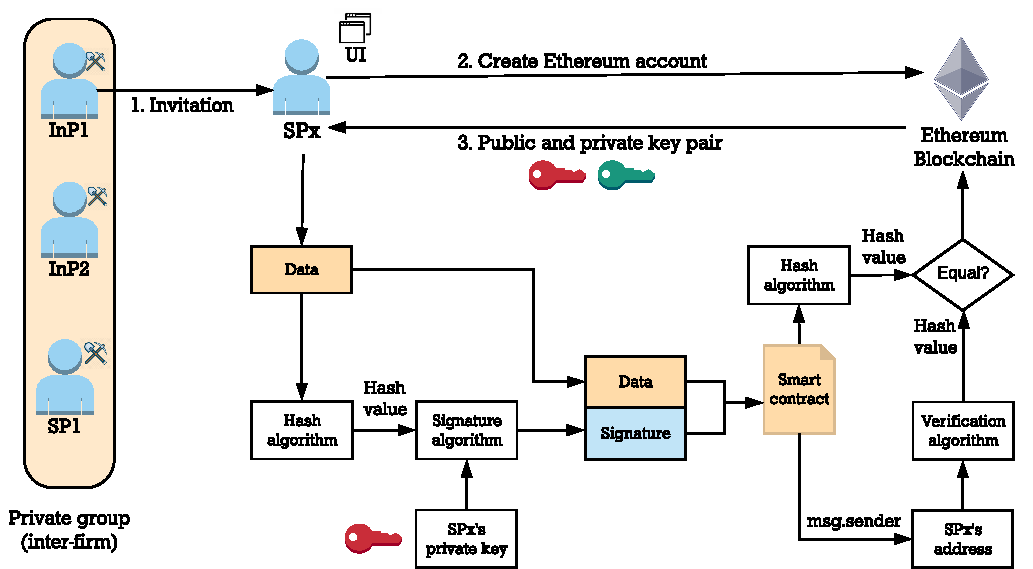
\includegraphics[scale=0.8]{gfx/authentication_design}    
  	\caption{Our authentication design and used public-key cryptography.}
  	\label{fig:authenticationDesign}
\end{figure}

Furthermore, to validate the origin and integrity of the messages, users must always digitally sign their operations, by providing a \textbf{digital signature}. In particular, Ethereum uses the \textit{Elliptic Curve Digital Signature Algorithm (ECDSA)} \citep{johnson2001elliptic}. In this process, see Figure \ref{fig:authenticationDesign}, a sender uses his private key to sign a hashed version of the data, which produces the signature. This signature, together with the original data, is sent to the receiver, who uses the sender's address (related to public key) and the data to verify that the information has been signed by who claims to be the owner and that the content has not been altered (hash value comparison).

It is important to note that smart contracts, if well-defined, provide security in terms of access control and confidentiality. Despite the fact that Ethereum users can create and own smart contracts, the content is not always accessible or alterable. For instance, when users are not willing to broadcast the contract's information or simply to avoid that every party is able to alter the state of the contract. Thus, these operations can be restricted only to a set of users, whose addresses need to be known by the contract account. In our VNE scenario, the matched InPs are the only users allowed to bid on specific resources.

Although the blockchain is a distributed technology, where the actors do not need to know or trust each other, thanks to cryptography, a secure and unalterable communication between all the participants is achieved. In addition, since Ethereum uses smart contracts, the data access can also be restricted.

\subsection{The Vickrey Auction Model} \label{vickrey}

In section \ref{auctionMechanisms}, after reviewing different auction types, we have concluded that a \textbf{one-sided reverse Vickrey auction} seems to be the most suitable for brokerless virtual network embedding. In the following, a more thorough examination in adapting this auction model to the multi-provider VNE scenario with LID is presented.

Firstly, we seek an efficient virtual network partitioning where the requested virtual nodes are assigned to the participating InPs, such that the VNE costs are minimized. Despite an auction could use a multi-dimensional process, i.e. more parameters, in this thesis, only the price quotes of the notified InPs will be used to determine the minimum VNE cost. Hence, the InPs act as sellers, who submit bids for the services requested by the SP, and once the auction finishes, the VN is split between the winning InPs. In this section, our focus will be on the techniques and auction models applied for the VN partitioning. Table \ref{tab:notations} summarizes all the used notations.

\begin{table}[htbp]
	\myfloatalign \footnotesize
	\begin{tabular}{m{2cm} m{14cm}}
		\textbf{Symbol} & \textbf{Description}\\ 
		\hline
		$G^{R}$ & virtual network request formed by a set of virtual nodes $N^{R}$ and a set of bandwidth demands $d^{R}$  \\		$N^{R}$ & set of requested virtual nodes \\
		$d^{R}$ & set of bandwidth demands between the virtual nodes $i,j \in N^{R}$ \\
		$N_i$ & virtual node $N_i \in N^{R}$ \\
		$N^{t}_i$ & virtual node $N_i$ type \\
		$d_i$ & virtual node demand for node $N_i$ \\
		$d_{ij}$ & bandwidth demand $d_{ij} \in d^{R}$ between the requested virtual nodes $i,j \in N^{R}$ \\
		$P_l$ &  $l$ virtual nodes groups \\
		$u_{i}$ & upper bound cost for the virtual node $N_i$ \\
		$u_{G}$ & upper bound cost for the virtual network $G$ \\
		$l_{i}$ & desired location for the virtual node $N_i$ \\
		$b_n(N_i)$ & $n's$ bid value for the virtual node $N_i$ \\
		$b_n(G)$ & bid value for the virtual network $G$ \\
		$v_n(N_i)$ & $n's$ real cost for the virtual node $N_i$ \\
		$v_n(G)$ & $n's$ real cost for the virtual network $G$ \\
		$C_n(N_i)$ & cost of virtual node $N_i$ when assigned to InP $n$ \\
		$C_n(G)$ & cost of virtual network $G$ when assigned to InP $n$ \\
		$C^{*}(G)$ & minimum cost of virtual network $G$ \\
		$\gamma_n(N_i)$ & InP $n$ profit margin at the time of bidding on virtual node $N_i$ \\
		$\gamma_n(G)$ & InP $n$ profit margin at the time of bidding on virtual network $G$\\
		$G^{S}$ & substrate network formed by a set of substrate nodes $N^{S}$ and a set of links $L^{S}$\\
		$N^{S}$ & set of substrate nodes \\
		$L^{S}$ & set of substrate links between the substrate nodes $i,j \in N^{S}$ \\
		$\alpha_{s^{*}}(N_i)$ & dynamic cost for embedding $N_i$ in the paired substrate node $N_s^{*}$ \\
		$\beta_{s^{*}}(L_{ij})$ & dynamic (fixed in evaluation) cost for sharing the paired substrate link $L_s^{*}$ \\
		\hline
	\end{tabular}
	\caption{Notations.}
	\label{tab:notations}
\end{table}

Since in our scenario SPs request the embedding of different virtual nodes $N_i \in N^{R}$, we are facing a multi-unit auction. Thus, before defining the minimum VN cost $C^{*}(G)$ using the \textit{one-sided reverse Vickrey} auction, it is important to note that $n = 1,...,N$ InPs can submit bids per virtual node $b_n(N_i)$ or for a group of virtual nodes $b_n(P_l)$, where $P_l$ are the $l = 1,...,2^{k}-1$ possible virtual nodes combinations. 

\begin{itemize}
 	\item \textbf{Per virtual node:} In a Vickrey auction with multiple items, the simplest form to bid is submitting a quote for each unit. In our scenario, these units are virtual nodes and in contrast to standard auctions, the \textbf{lowest bid} wins the service, inasmuch as the SPs are the ones who pay for the services offered by the InPs. Thus, to ensure not ending up with inflated prices, the SPs denote either an upper bound cost per virtual resource $u_{i}$, or a global one for the virtual network $u_{G}$, where $u_{G} = \sum_{i=1}^{k}u_i$. For instance, let $v_n(N_i)$ and $b_n(N_i)$ be, respectively, bidder $n$'s real cost and bid value for the virtual resource $N_i$. Since it is a \textit{low-bidding second-price auction}, the cost $C_n(N_i)$ that the service provider pays to InP $n$, is given by Equation \ref{eq:Cnkcost}. This value must also include the link costs, which after being evaluated by the InPs, are subsequently added to the quoted price $b_n(N_i)$. In this thesis, we assume that the intra-link costs within an InP are negligible and that the inter-links, due to the lack of information of the other InP's substrate topologies, must be roughly estimated by the InPs. On the other hand, it is important to note that in our system, when $b_n(N_i) = b_j(N_i)$, the first bidder will be the provisional winner. For instance, in an English auction the same decision is taken since when a bidder overcomes a price, the next participant must always bid a higher value than the current one. Thus, the InP's goal is to smartly quote $b_n(N_i) = v_n(N_i) \times [1 + \gamma_n(N_i)] \leq u_{N_i}$, where the symbol $\gamma_n(N_i) \in [0,1]$ represents the profit margin that InP $n$ takes at the time of bidding for $N_i$, knowing that the lower $\gamma_n(N_i)$ is, the higher the probability of winning, although at a smaller revenue. The cost $C_n(N_i)$ that a SP pays to InP $n$ is given by:

   \begin{equation} \label{eq:Cnkcost}
   C_n(N_i) =
   \begin{cases}
    \min b_j(N_i), & b_n(N_i) < b_j(N_i) \leq u_{i} : \ \forall j \neq n, \ \exists b_j(N_i) \neq \infty \\
    b_n(N_i), & b_n(N_i) < b_j(N_i) \leq u_{i}: \ \forall j \neq n, \ \nexists b_j(N_i) \neq \infty \\
    \infty, & \text{otherwise } \\
  \end{cases}   
   \end{equation}
   
   \item \textbf{Per group of virtual nodes:} The Vickrey auction model behaves differently when a seller offers a package of items at a lower price, also called package pricing. In this context, rather than ending up paying the second price of the auction, the winner pays the \textbf{opportunity cost} for the units won, or in other words, the "damage" that his bids impose on the rest of the bidders. Formally, it is described as follows. Let $x$ be a vector of outcomes again with $n = 1,...,N$ players bidding $b_n(X_n)$. The mechanism will seek for the outcome $x^{*} \in argmax_{x_1,...,x_N} \sum_{n} b_n(X_n)$ that maximises the efficiency. Then, the cost for bidder $n$ will be $p_n = \sum_{j \neq n} b_j(x^{*}_{-n}) - \sum_{j \neq n} b_j(x^{*}_{j})$, where the term $x^{*}_{-n}$ refers to the most efficient outcome without the presence of bidder $n$. Generally speaking, this expression can be seen as the result of the auction when bidder $n$ is not participating in the auction, minus the total cost for the other bidders when $n$ participates. However, in \citep{ausubel2006lovely}, it has been proven that the Vickrey auction for multiple items suffers from serious weaknesses, e.g. zero revenues or unfair prices, which results in a poor performance. Due to the high degree of complexity, in this thesis, we investigate the package pricing when an InP bids for the whole VN network $C_n(G)$, rather than for partial biddings $C_n(P_l)$. For instance, as shown in Figure \ref{fig:vickrey} example, we will just consider bids for the entire network $b_n(ABCD)$ and not the other possible combinations, such as $b_n(AB)$ or $b_n(AB) + b_n(ABC)$. Hence, in this case, the cost $C_n(G)$ will be treated exactly as in the per virtual node auction, represented as:
    
  \begin{equation} \label{eq:Gcost}
   C_n(G) =
   \begin{cases}
    \min b_j(G), & b_n(G) < b_j(G) \leq u_{G} : \ \forall j \neq n, \ \exists b_j(G) \neq \infty\\
    b_n(G), & b_n(G) < b_j(G) \leq u_{G}: \ \forall j \neq n, \ \nexists b_j(G) \neq \infty \\
    \infty, & \text{otherwise } \\
  \end{cases}
  \end{equation}
\end{itemize}

 Finally, an algorithm that combines individual bidding and package pricing, and calculates the minimum VN cost $Cm(G)$, is now designed. Firstly, in case no bid per package is provided, the cost for the VN network can be generally expressed as $C^{*}(G) = \sum_{i=1}^{k}C_n(N_i)$, which is the sum of all minimum virtual nodes costs. However, when the two bidding types are used, the minimum cost is calculated as follows:

  \begin{equation} \label{eq:Cmcost}
        	C^{*}(G) = \min\{C_n(G), \sum_{i=1}^{k} C_n(N_i)\}
  \end{equation}

The last expression shows that the system first computes independently an individual and a package auction. Afterwards, the resulting costs for these two tenders are compared, whose minimum value gives us the final VNE cost $C^{*}(G)$. In case $C_n(G) = \sum_{i=1}^{k} C_n(N_i)$, the virtual network will be embedded to the InP offering package pricing, since the performance is always better within a single InP. Moreover, the common InPs bidding strategies and the encountered weaknesses of the Vickrey model for package pricing, need to be investigated in this design. Algorithm \ref{alg:algorithm1} shows the pseudocode of the InP $n$ resource matching and subsequently bidding strategy, where $N^{t}_i$ corresponds to the virtual node type of $N_i$.


 \begin{algorithm}
  \caption{InP $n$ resource matching and bidding strategy}
 \label{alg:algorithm1}
  \begin{algorithmic}[1]
 \IF{$N_s \leftarrow \forall l_i \land \forall N^{t}_i$} 
 	\STATE{\Return $b_n(G) = v_n(G) \times [1 + \gamma_n(G)] \leq u_{G}: \ v_n(G) = \sum_{i=1}^{k} v_n(N_i), \gamma_n(G) \in [0,1] $}
 \ELSE
  	\FOR{$N_i \in N^{R}$}
 	 \IF{$N_s \leftarrow l_i \land N^{t}_i$}
 	  \STATE{$b_n(N_i) = v_n(N_i) \times [1 + \gamma_n(N_i)] \leq u_{N_i}: \ \gamma_n(N_i) \in [0,1]$}
 	 \ENDIF
 	\ENDFOR
 	\State \Return $b_n(N^{R})$
 \ENDIF
 \end{algorithmic}
\end{algorithm}

Firstly, according to Algorithm \ref{alg:algorithm1}, an InP bids either for the entire virtual network $b_n(G)$ or for individual virtual nodes $b_n(N_i)$, depending on the amount of paired resources. In other words, if all the virtual nodes locations $l_{i}$ and types $N^{t}_i$ are matched with certain InP substrate nodes $N_s$, then the system enables that the infrastructure provider bids for the entire virtual network. If not, an InP is only allowed to quote prices for the paired virtual nodes.

To better explain the bidding strategy of Algorithm \ref{alg:algorithm1}, it is worth taking a look at the example from Figure \ref{fig:vickrey}. There, four InPs are competing to win virtual nodes $\{A, B, C, D\}$, each using profit margin values of $\{\gamma_1 = 0.6,\gamma_2 = 0.\wideparen{1},\gamma_3 = 0,\gamma_4 = 0.2\}$. In this example, the profit margins are identical for each $N_i$ and $G$. At the end of this auction, since the individual quotes are lower than the package pricing offer $C^{*}(G) = min\{30, 29\}$, the virtual network is partitioned across different InPs, i.e. $A \rightarrow InP_1, B \rightarrow InP_1, C \rightarrow InP_4, D \rightarrow InP_3$.  In addition, the prices that the SP must pay to each InP are the ones resulting from the \textit{low-bidding second-price auction} $C_n(N_i)$. 

\begin{figure}[bth]
	\centering
	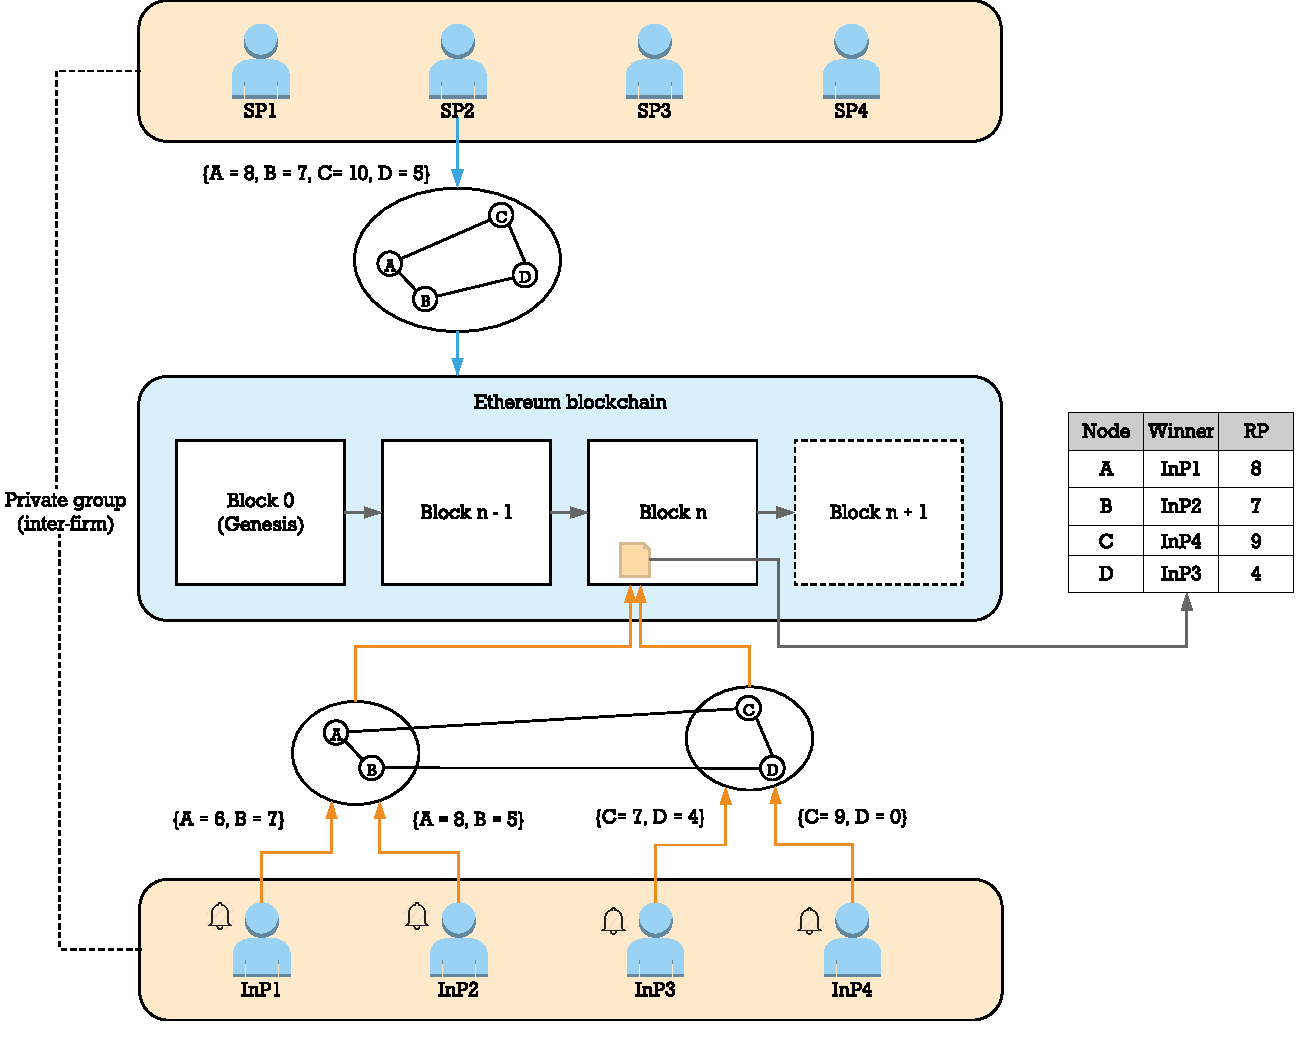
\includegraphics[scale=0.75]{gfx/vickrey}    
  	\caption{Our designed auction algorithm that combines the Vickrey model with package pricing.}
  	\label{fig:vickrey}
\end{figure}

In the above-mentioned example, is important to note that although $InP_1$ applies the highest profit margin, it is the one with the best outcome. Thus, since the virtual node and virtual network bids are determined first by $v_n(N_i)$, which is also used in $v_n(G) = \sum_{i=1}^{k} v_n(N_i)$, and secondly by $\gamma_n(N_i)$ and $\gamma_n(G)$, these values need to be examined:

\begin{itemize}
 \item \textbf{Real cost $\mathbf{v_n(N_i)}$}: Since network virtualization is a real-time process where the demand and availability of the resources are constantly changing, our approach encourages that users apply \textbf{dynamic pricing models}. A dynamic pricing model, in contrast to fixed pricing, is a strategy where the prices are flexibly adapted to the current market demands, rather than always charging the same costs. In our approach, InPs could use algorithms that take into account the SP demands and the current availability of the resources, to better define their product prices, and hence, to have a better market positioning. For instance, they could use the demand and supply principle in microeconomics, which states that if the demand for a product short in supply is high, the price increases. In our scenario, this demand is related either with the computing or the bandwidth requirements, and the supply with the resource utilization. Thus, the real cost $v_n(N_i)$ is given by Equation \ref{eq:virtualNodeCost}, where $\alpha_{s^{*}}(N_i)$ and $\beta_{s^{*}}(L_{ij})$ are the dynamic prices for the paired substrate node $N_s^{*}$ and link $L_s^{*}$, and whose values will be updated according to the resource availability (see chapter \ref{ch:evaluation}). Apart from demand and supply, InPs could also use automated processes based on other factors, such as competitive pricing or customer behaviors. In the former, since the reserved prices for the virtual nodes are publicly known when an auction finishes, it allows InPs to learn from competitors in order to be more proficient in incoming auctions. In the latter, the virtual node upper bound costs entered by the SPs on their VN requests, can also be used to adjust the InP prices on customers needs. Overall, due to the high elasticity of the prices, InPs should recalculate periodically their costs, in order to compete in the modern market. This cost estimation can be performed based on many other factors, which can be thoroughly examined in future research.
 
  \begin{equation} \label{eq:virtualNodeCost}
	v_n(N_i) = \alpha_{s^{*}}(N_i) + \sum_{j = 1}^{k} {\frac{\beta_{s^{*}}(L_{ij})}{2}} \qquad \forall j \in N^{R}, \ \exists d_{ij} \neq \infty : \ i \neq j
  \end{equation}
  
  \item \textbf{Profit margins $\mathbf{\gamma_n(N_i)}$ and $\mathbf{\gamma_n(G)}$}: The profit margin is a measure to indicate the profitability of a product, which is extracted from the net profit divided by the cost. Equations \ref{eq:profitmarginNode} and \ref{eq:profitmarginGraph}, give the values of the profit margins for a virtual node and for the entire network. It is important to note that these values are provisional (at the time of bidding), since if a second lowest quote exists, as it is a \textit{second-price auction}, the values $b_n(N_i)$ and $b_n(G)$ will be replaced by $C_n(N_i)$ and $C_n(G)$ respectively. Typically, a high-profit margin produces a higher revenue, although at a smaller probability of winning. Nevertheless, from the example in Figure \ref{fig:vickrey}, we can observe that if an InP performs a good market research (most probably $InP_1$), it can also obtain virtual nodes through high-profit margins. Thus, in chapter \ref{ch:evaluation}, we will examine how the risk taken by the InPs at the time of determining the profit margins, affects the VN embedding outcome.

\begin{equation} \label{eq:profitmarginNode}
	\gamma_n(N_i) = \frac{b_n(N_i)- v_n(N_i)}{v_n(N_i)} \qquad \gamma_n(N_i) \in [0,1]
  \end{equation}
  
\begin{equation} \label{eq:profitmarginGraph}
  \gamma_n(G) =  \frac{b_n(G)- v_n(G)}{v_n(G)} \qquad \ \  \gamma_n(G) \in [0,1]
\end{equation}

\end{itemize}

Lastly, we analyze the weaknesses of the Vickrey auction model for package pricing in our design \citep{ausubel2006lovely}, and observe how the potential attacks on Internet auctions could hinder our system performance \citep{boyd2000security}:

\begin{itemize}
 \item \textbf{Bidder non-monotonicity:} Adding other bidders in a \textit{Vickrey auction} with package pricing can result in low or zero revenues, such that bidders pay the opportunity cost. Hence, the system has potential vulnerabilities that the bidders can exploit. In our design, as the virtual network and the corresponding virtual nodes are treated as single independent items, adding more bidders will only increase the resource competition.
    \item \textbf{Multiple bidding identities:} In many Internet auctions, a single bidder can use multiple pseudonyms or accounts to bid and increase their profits. In our system, as users can only be registered once (through an invitation), it is not possible for an InP to have multiple Ethereum accounts to compromise the final outcome. Thus, this is a controlled system where InPs, such as Deutsche Telekom or Swisscom, are identified by a single account.
    \item \textbf{Bid shielding:} It consists in the withdraw of bids in the last minute. Since our application interacts with a blockchain, where submitted data is immutable, this has no influence on the system.
    \item \textbf{Bid sniping:} The auctions started by the SPs have a fixed duration, after which no further bids are accepted. In this case, an InP could enforce a denial of service attack, by sending multiple last-minute bids, in order to prevent that the system computes other bids and hence, winning the auction. For this reason, in our system, each InP will have to first pay his bid to the smart contract, and a percentage of this total quantity will be refunded after the sealed bid is opened.
\end{itemize}


\section{Summary}

Virtual network embeding (VNE) enables SPs to embed virtual nodes across different InPs to create customized virtual networks. Typically, these InPs are not willing to disclose detailed information about their resources availability or network topologies, which directly affects the VNE performance. In addition, the service providers seek to minimize VNE embedding costs, such that the VN partitioning is treated as a cost minimization problem.

In this thesis, an approach to improve the VNE throughput under the limited information disclosure scenario has been introduced. More precisely, a complete system using the Ethereum blockchain has been presented, which thanks to smart contracts, enables the creation of new embedding strategies to facilitate the service negotiation between the InPs and SPs. In our case, an algorithm adapted from the Vickrey auction model has been designed, which improves the VN partitioning efficiency. In the following chapters, the implementation of this design will be evaluated.

We do not claim that our approach is the only way of performing VN partitioning. However, it enables brokerless VN embedding in a distributed environment. Furthermore, to the best of our knowledge, this is the first approach using blockchain in the VNE context, and thanks to smart contract's flexibility, it can serve as a starting point for more upcoming investigations.

%*****************************************
\chapter{Implementation}
\label{ch:implementation}
%***************************************** 

In the following, the implementation of a brokerless VNE system under limited information disclosure is introduced. In chapter \ref{ch:design}, after investigating the different types of blockchain platforms, we have presented a complete design for the system architecture, which uses the Ethereum blockchain, and hence, smart contracts. 

In this part, we first define the design decisions and environment where our approach is implemented. Afterwards, we present the system architecture, describing how a hybrid blockchain with multiple nodes is configured in the Ethereum platform, and how the authentication system works. 

In addition, we thoroughly explain the two developed contracts for our design: the Users and Vickrey contract. The first acts as a permanent database contract, with the only logic of updating its state with new user data. The second is an application contract used as a template for every auction that is started (multiple Vickrey contracts). In particular, the code is equal for all the created contracts, although with different states restricting the user interaction to the allowed ones. Thus, through these contracts, we represent the tailored Vickrey auction model, in order to improve the VN partitioning efficiency and minimize the costs between the InPs and SPs. Finally, we discuss the implementation workflow, that is, the interactions between the system components, along with the limitations observed in our implementation.

\section{Design Decisions}

In section \ref{smartContractsAndEthereum}, we have discussed the reasons why is logic to choose Ethereum as the main platform of our hybrid blockchain, among which, we highlight the maturity and the building simplicity of the project. Thanks to this, the blockchain concept is fastly understood and tested, resulting in a straightforward and intuitive scenario setup. In addition, a large number of starter tutorials can be found since Ethereum is utilized by many users on the Internet. Thus, the basic steps for becoming familiar with Ethereum are extremely facilitated, which help us on start writing our first smart contracts.

In the design system architecture (Figure \ref{fig:designWorkflow}), we have stated that for automation, each user efficiently interacts with the blockchain through an API. Therefore, it is important to first study the environment workflow, i.e. which technologies enable clients to create, read and update data from the blockchain.

The first aspect to consider is how to run the blockchain nodes that maintain the BC platform. These nodes are responsible for downloading the blockchain into the system on a regular basis, verifying and processing the incoming transactions and syncing this information with the other nodes. However, there are multiple clients that run the Ethereum clients/nodes across different operating systems, such as Go-Ethereum \citep{GoEthereum2014}, Parity \citep{Parity2016} or Pyethapp \citep{Pyethapp2015}, written in Go, Rust and Python respectively. Despite all those packages are experimental, in our thesis, we use \textbf{Go-Ethereum (Geth)} since it is the official client software provided by the Ethereum Foundation (no third parties). Moreover, Geth provides a simple set up for multiple clients in private networks, see section \ref{privateNw} for more details.

After having configured the blockchain, the next step is to understand how to write, compile and store the smart contracts. Firstly, as outlined in the design chapter, there are mainly two programming languages for writing smart contracts: Solidity (JavaScript) and Serpent (Python). At the time of writing, Serpent has been deprecated in favor of Viper \citep{Viper2017}, a new experimental Python programming language developed by the Ethereum Foundation. Despite Viper is approached to be simpler with more auditable and secure smart contracts, it currently does not have a large number of features, documentation and community support due to its low maturity. Thus, as we seek for quick usability to start testing our scenario, the most widely supported, documented and stable language, is \textbf{Solidity}. 

\begin{figure}[bth]
	\centering
	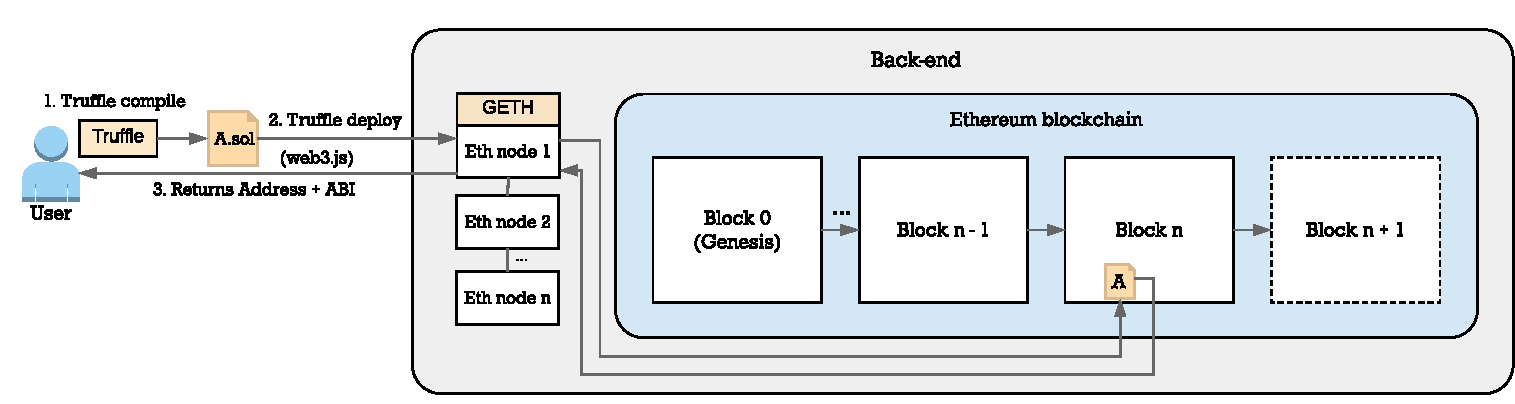
\includegraphics[width=1\linewidth]{gfx/Smart_contract_workflow}    
  	\caption{Smart contract compilation and deployment using the Truffle framework.}
  	\label{fig:smartContractWorkflow}
\end{figure}

Besides that, Solidity can be integrated with great frameworks, such as Remix\footnote{\url{https://remix.ethereum.org/}}, which is a browser-based compiler and Integrated Development Environment (IDE) that enables the creation, debugging and testing of Solidity smart contracts. Nevertheless, since users need a friendly GUI to perform different actions, apart from interacting with smart contracts, we cannot use a browser IDE for our final system application. In our case, we will only utilize Remix for the testing and debugging of smart contracts. 

Fortunately, there are several frameworks that simplify the complexities of compiling, deploying and testing smart contracts into the blockchain, as well as reaching and accessing them subsequently from the application. Among those, we want to highlight Truffle \citep{Truffle2015} and Embark \citep{Embark2016}. They are both comparable in terms of features and usage simplicity. However, Embark allows a quite easy development in front-end applications, although, in other systems (e.g. back-end server), the features integration is more complex. On the contrary, Truffle can also be placed in these systems, providing a straightforward project creation, contract deployment and interaction on private networks, with plenty of detailed documentation on the Internet. Therefore, as our application may grow over time with new functionalities, \textbf{Truffle} seems to be the most appropriate solution.

To better explain the workflow on deploying smart contracts, Figure \ref{fig:smartContractWorkflow} reflects an example of a user that uploads one smart contract through an Ethereum node. The process comprehends the following steps: Firstly, after writing the smart contract, the user compiles it. Consecutively, if no error appears, the user deploys the contract into the blockchain. Finally, once placed into the last block, the Ethereum node returns the address of the created contract together with the application binary interface (ABI) in JSON format. From now on, the user can request and modify the state of the contract using the corresponding ABI and address through web3.js. \textbf{Web3.js} is a JavaScript library that enables the interaction with local or remote Ethereum nodes, using an HTTP or IPC connection. In addition, due to the changes in deployment as the project evolves, truffle also enables defining migrations, which are JavaScript files that help users to deploy the desired contracts into the network. 

At this point, we have already compared and selected the technologies used for the deployment of our Solidity smart contracts into the Geth blockchain. Nevertheless, the definition of another fundamental part of our system is still required: the front-end. Since we do not observe any advantage on users having the presented application on mobile phones, we opted for developing a traditional web application rather than a mobile application. In this way, users can easily interact with the blockchain by accessing the application on their browsers. 

Thus, the first and main requirement for the front-end is that the programming language is accepted and supported by most of the browsers without the need of compilers or plugins. In web development, JavaScript is the most used, and hence, better positioned in this respect. Nowadays, there are many JavaScript frameworks extending the HTML and CSS capabilities, such as AngularJS, ReactJS or VueJS. Due to its consistency, efficient productivity, simplicity, and maintainability, we have chosen \textbf{AngularJS} as the default language for our web application. AngularJS is a popular JavaScript-based open-source framework released by Google, with a large number of features and a built-in functionality for creating responsive and reactive web applications.

Lastly, we need a computer software that connects all the defined components, handling and transmitting the requests to the blockchain nodes: a \textbf{middleware (MW)}. Thanks to the middleware, the Geth nodes will be configured to only accept requests initiated from the domain of this component, which prevents that the system suffers from many security issues. Thus, Truffle will be placed on the middleware and the web application will use it as a gateway for the API management. This middleware could also check the user's identity (authentication system), in order to ensure that only the allowed peers interact with the Ethereum nodes. Regarding the programming language, as our environment has been mostly developed in JavaScript, we employ \textbf{Node.js}, which is an open-source JavaScript environment that runs on the server side.

Apart from the reasons mentioned above, a MW enables the integration and correlation of different data sources (blockchain and non-blockchain events) in real time, such as blockchain clients, databases, partner APIs or a publish/subscribe system. Later on, this data could be used for the InPs maintaining the application, to find insights and patterns in historical data, i.e to apply machine learning techniques. Therefore, a middleware is a key success factor for managing a blockchain project, and later to integrate it with existing services and platforms.

\section{Architecture} \label{architecture}

After having discussed the reasons for choosing certain technologies and software components, in Figure \ref{fig:archi}, we present an overview of our system architecture. As most of the web applications (webapp), the structure consists of two main components: the front-end and the back-end. The first can be run in a traditional centralized web server (e.g. AWS EC2 instance) or in a more distributed environment, such as the InterPlanetary File System (IPFS) \citep{benet2014ipfs}, which enables the hosting of decentralized applications (dapps) on the Internet. In particular, the front-end is formed by a webapp based on Angular 2, a more sophisticated version of Angular.JS, responsible for displaying on the browser the functionalities used for the clients (private group) to interact with the application. In addition, the front-end contains another fundamental element for the system functionality, a middleware, which can also be placed on the server. As explained in the section above, in order to manage the interaction with the Ethereum nodes, improve the system's security and further integrate the dapp with other services, we also set up the Truffle framework in the middleware.

\begin{figure}[bth]
	\centering
	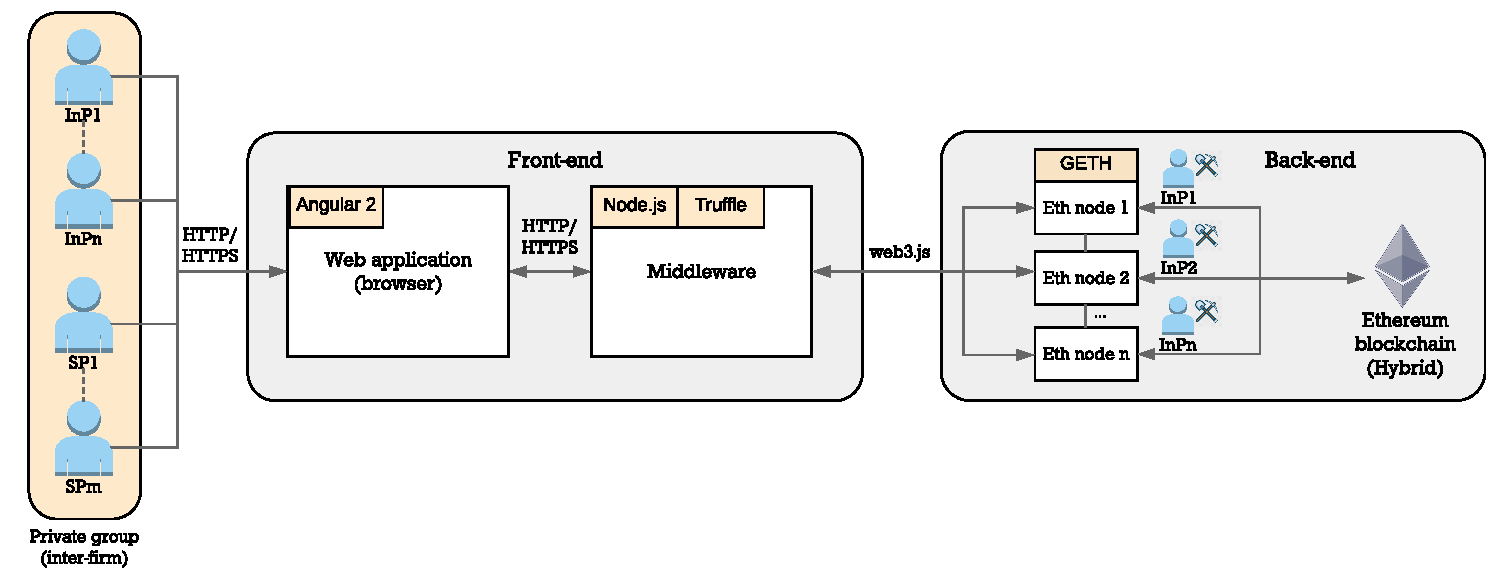
\includegraphics[width=1\linewidth]{gfx/Implementation_architecture}    
  	\caption{Architecture overview of the technologies and software components used for our system.}
  	\label{fig:archi}
\end{figure}

On the other hand, in Figure \ref{fig:archi}, we have placed together in the Back-end server, the different Geth nodes and the Ethereum blockchain. However, it is important to note that in our scenario, the different nodes are maintained and served by different firms, and most probably, domains. For instance, company A and B are responsible for controlling nodes 1 and 2, which are placed on http://www.companyA.com:3005 and http://www.companyB.com:3005 respectively. Another point to bear in mind is that every new Ethereum node must be subsequently added to the web3 configuration of the MW. If not, the system will become more centralized and prone to DoS attacks, with the transactions always sent to the same node. Nevertheless, this middleware does not to be immediately modified since all the transactions are added to a shared pool by all the Ethereum nodes.

Thus, in the following, we describe how to set up a hybrid blockchain where all the miners are synchronized and work coordinated.

\subsection{Hybrid Blockchain with Multiple Mining Nodes} \label{privateNw}

In the first place, to initialise a private blockchain separated from the public Ethereum chain, there are three components that need need to be customized:

\begin{enumerate}
	
	\item \textbf{Data Directory:} It is where the chain data of our blockchain is stored. In our case, each firm has a specific directory in the machine running the mining node, where all this information is saved.
	\item \textbf{Network ID:} It is a scalar value that identifies the customized network, which must be random but different than other predefined networks, such as 1 or 4 used for the Ethereum public main network or the public Geth Ethereum testnet respectively. In our environment, this value needs to be known for all the mining nodes.
	\item \textbf{Genesis Block:} The Genesis block, also called block 0, is the start of the Blockchain. It is hardcoded into the client in a file called genesis.json, whose content must be identical for all the mining nodes to ensure that they work on the same blockchain. Since it is written in JSON format, the specifications for the genesis block are written in key/value pairs. Despite most of these parameters are later on arbitrary, they need to be first defined in the genesis block \citep{GenesisParams}: (i) \textit{nonce}: Recap from \ref{mining_Transactions} that the nonce is a 64-bit hash, which proves that a sufficient amount of work has been performed on creating the next block header. (ii) \textit{mixhash}: It is an intermediary hash calculation (256-bit) used to determine if an attacker mines blocks with incorrect nonces. (iii) \textit{timestamp}: A scalar value equal to the current Unix time to identify when a block is mined. The values introduced until now are meaningless in the genesis block, since they will be later on arbitrary or specific to the current time (timestamp). (iv) \textit{difficulty}: An integer that defines the increase or decrease of the mining block complexity depending on the timestamp differences between the current and the parent block. (v) \textit{parentHash}: The keccak 256-bit hash of the parent block header. This is meaningless in the genesis block, since block 0 has no parent. (vi) \textit{extraData}: An optional value with a maximum size of 32-bytes. (vii) \textit{alloc}: It is a list of accounts with pre-allocated Ether. (viii) \textit{coinbase}: A 160-bit address to which all the mining rewards are sent. In our case, as the mining rewards are divided between the different nodes this value is not set. (ix) \textit{gasLimit}: A value equal to the maximum gas for transaction.
\end{enumerate}


In Listing \ref{lst:JSONFile}, we present the genesis file used for our implementation. There, we define the \textit{difficulty} to be equal to 0x800, which is the minimum value for the Ethereum PoW (explained later in section \ref{resultsBlock}). Note that in PoW, a miner needs to find a valid block header, whose cryptographic hash is less than $\frac{2^{224}}{d}$, where $d$ is the block difficulty (Equation \ref{eq:proofOfWork}). Thus, a small difficulty gives us a higher value for this term, which results in a higher probability of finding the block header. In chapter \ref{ch:evaluation}, we will further examine how this parameter influences the block generation time, and which is the most suitable value for a private network.
\newline

\begin{lstlisting}[language=JSON,caption={Genesis file used for our implementation.},label={lst:JSONFile}]
{
    "nonce": "0x0000000000000042",
    "timestamp": "0x0",
    "parentHash": "0x0000000000000000000000000000000000000000000000000000000000000000",
    "extraData": "0x00",
    "gasLimit": "0x8000000",
    "difficulty": "0x800",
    "mixhash": "0x0000000000000000000000000000000000000000000000000000000000000000",
    "alloc": {
    },
    "config": {
        "chainId": 987654321,
        "homesteadBlock": 0,
        "eip155Block": 0,
        "eip158Block": 0
    } 

}
\end{lstlisting}

Apart from the already introduced fields, in our genesis file, we have introduced a \textit{config} parameter, which specifies the configuration of the Ethereum network and has no relation with block 0. In particular, \textit{chainId} is a random number different from the network ID, which specifies the working chain. For instance, a peer can use the network ID 58342 but later mine in chain 1. If we set the \textit{homeSteadBlock} field to 0, it implies that the chain is using the Homestead release of Ethereum, which is the same of the main Ethereum network. Finally, the EIP parameters stand for Ethereum Improvement Proposals, from which we use the \textit{eip155Block} and \textit{eip155Block} that are used to prevent replay attacks and modify the way to deal with empty accounts (less space in BC) respectively.

After having defined the genesis file, one Ethereum node must build it in order to start running the blockchain. An example of the two commands needed are illustrated below:
\newline

\begin{lstlisting}[language=JSON,caption={Example of the two Geth commands used to start running the blockchain.}, label={lst:GethCommands}]
$ geth --datadir <path-to-directory> init genesis.json
$ geth --port 3000 --networkid 58342 --datadir="<path-to-directory>" --maxpeers=3 --rpc --rpcport 8545 --rpcaddr 127.0.0.1 --rpccorsdomain "http://localhost:8000" --rpcapi "eth,net,web3,personal" --gasprice "0" --nodiscover console
\end{lstlisting}

The first command specifies the data directory where the blockchain data is initialized and stored, and the second starts running the blockchain with the specified parameters. In this example, the blockchain is configured to run locally in port 3000 and with network ID 58342. In addition, a gas price equal to 0, means that the transactions in the blockchain have not cost. Since we are building a private blockchain with different users, it is not logical to charge those when they are performing operations. For instance, when a user registers to the application or when a SP begins a new auction. Also, adding the field --nodiscover disables the peer discovery mechanism, i.e. nodes are only connected by manual addition. 

After executing these commands for each of the Ethereum clients, which should have the same genesis file and network ID but different domains, ports and data directories, these nodes need to be synchronized. To achieve this, Geth supports a feature called static nodes, which can be configured into \textit{<path-to-directory>/static-nodes.json}. These static nodes are added through the so-called \textbf{Enodes}, which are Ethereum nodes written in a URL scheme. In Listing \ref{lst:ENodes} an example of a \textit{static-nodes} file in a blockchain client, which adds two other Enodes is presented.

Once all the nodes are connected and have synchronized the blockchain status, they can start to mine all the incoming requests. The distribution of the mining privileges between these nodes will be later evaluated in chapter \ref{ch:evaluation}, where a JavaScript file is preloaded on each of these clients.

\begin{lstlisting}[language=JSON,caption={Example of a \textit{static-nodes.json} file that adds two other blockchain nodes.}, label={lst:ENodes}]
[
"enode://38dd47f0ed04ec88ede2f75970da08f23ca87de8f96bf576dc769b0f9df807782d3729bc83b99042a3eb193ff 091cb4715a0906e5e902fb5adc04af91f3a7ba7@[::]:3010?discport=0",

"enode://dcd4a6714af990cc036dcb3b46c8ac6f929d7b9c1119ba3bdf8ffde9252fa17204bac84c3afae9c53b38c4a 0dacccd2c52ac832ec723c5ff5e29546402c09737@[::]:3015?discport=0"
]
\end{lstlisting}





\subsection{Authentication system}

In section \ref{authenticationSystem}, we have presented the conceptual design of how a user is registered and authenticated in our system. More specifically, the first is performed through a user invitation and the second providing a digital signature to validate the origin and integrity of the messages. In the following, we introduce the implementation of such a system in our architecture, in which the web application sends the corresponding information to the middleware, who later uses web3 to interact with the Ethereum nodes.

Firstly, a consortium of InPs invites a user to join the network, e.g. a service provider shares a link that allows the creation of an Externally Owned Account (EOA) by entering a password. Afterwards, the user receives the created address, which can only be unlocked by entering this password. In Geth, an account needs to be unlocked in order to send transactions from it to the blockchain. Therefore, for not entering the password each time a user sends data to the BC, we create an authentication system, in which the corresponding account is directly unlocked for the desired time when a user logs in.

Nevertheless, before a user is logged in, he needs to register to the application entering the following fields: (i) an email, (ii) the previously created Ethereum address and (iii) the user's role to later distinguish between InPs and SPs. Note that the Ethereum address is extremely important, since if a user forgets this address, all the information regarding the account, e.g. ETH earned, will be lost. After being successfully registered to the application, now the user can sign in, and hence, utilize the application. This process employs the digital signature concept, although it slightly varies depending on the technology used (e.g. Parity or TestRPC). In Figure \ref{fig:authImplem}, we illustrate how this mechanism works, where SPx authenticates to the system by entering the Ethereum address and the password to unlock this account on the browser.

The cycle starts with hashing a random data, which is later signed with the unlocked address to generate a signature (web3.eth.sign(address, hash value)). This signature can only be performed by the owner of the address since he is the only one that knows the password to unlock this account. Subsequently, the signature is sent via HTTP together with the hash value and the address to the middleware, which is responsible for authenticating the client. This authentication consists in recovering the Ethereum address from the signature and a specific hash of the data. If the obtained address matches the one provided on the HTTP request, or in other words, if the user is proved to be the owner, a JSON web token is generated. In particular, a self-contained token is provided, which as the name suggests, includes user information (address). Therefore, from now on, the user attaches this token on the HTTP header for every request sent to the blockchain. This token is validated by the middleware, who decrypts it through the secret key already used to encrypt it (symmetric encryption). In addition, once a user sends a request, the token is updated with a new expiration time equal to one hour.

\begin{figure}[bth]
	\centering
	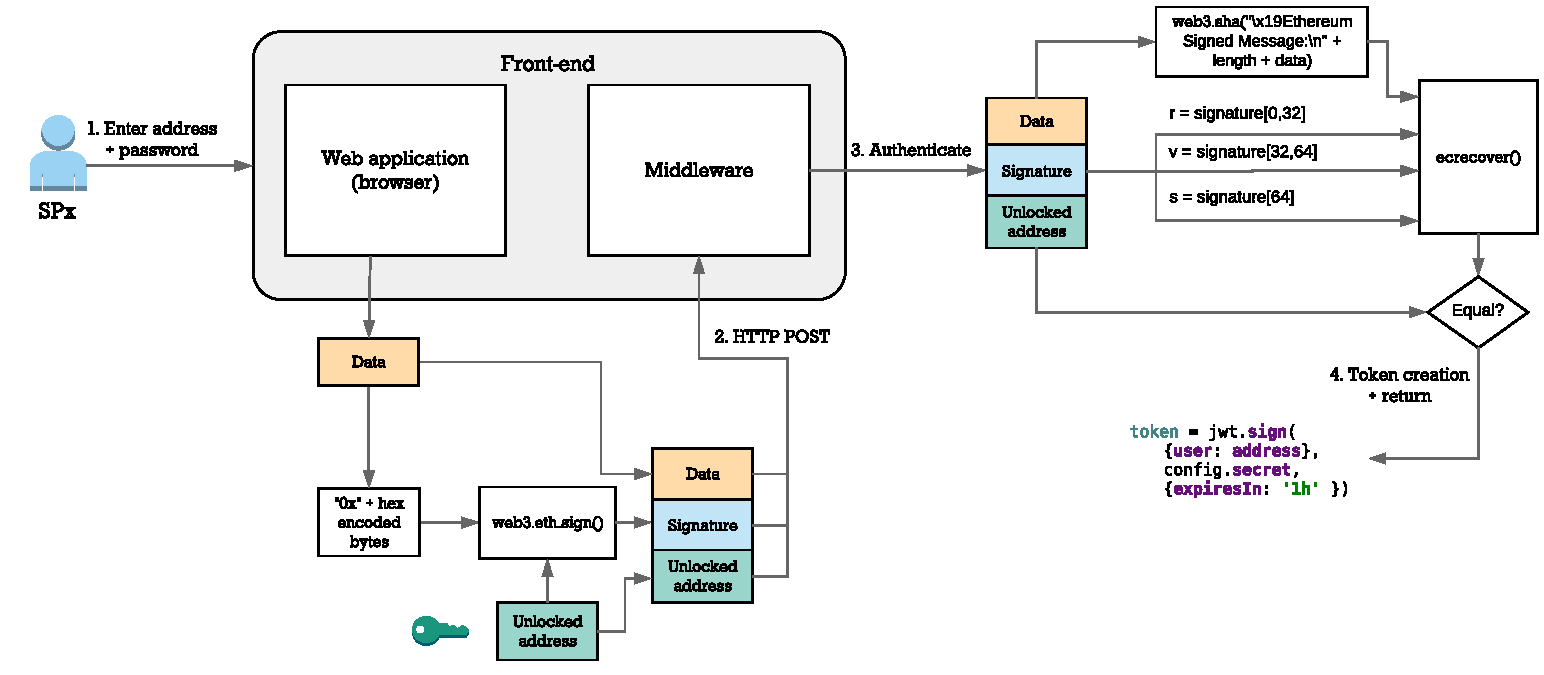
\includegraphics[width=1\linewidth]{gfx/Authentication_implementation}    
  	\caption{Overview of the implemented authentication system.}
  	\label{fig:authImplem}
\end{figure}

To summarize, thanks to the developed middleware and the web tokens, in the authentication process, the Ethereum clients are only responsible for creating the Ethereum accounts and subsequently unlock them. This ensures that the Ethereum clients, and hence, the smart contracts are efficiently used for only specific tasks, and that the users do not spend time on entering the login credentials for each transaction. For instance, performing the signature verification in a contract requires a higher computational effort, which can lead to a system overload if executed frequently.


\subsection{Users Contract}

In the design of the system architecture, see Figure \ref{fig:designWorkflow}, we have defined a permanently requestable smart contract named \textit{Users}, whose responsibility is to store the participant's information used to match different virtual node types in specific locations. Given the importance of this contract, on the next pages, we present the fundamental data structures and functions that describe its functionality. To understand the code, it is assumed that the reader has a basic knowledge of JavaScript or even better Solidity.

To begin with the contract, we have defined the structs \textit{User} and \textit{UserAuction}, see Listing \ref{lst:UserContract1}. The first stores the email and role of the registered user and it is accessed by giving its Ethereum address (\textit{users} mapping). The second provides all the auctions (open and close) of a determined user by entering again the address as the key of the \textit{userAuctions} mapping. If the endTime is smaller than the current Unix time(), no more bids can be placed to the contract. 
\newline

\begin{lstlisting}[language=JavaScript,caption={Data structures related to the user data in the \textit{Users} contract. },label={lst:UserContract1}]
  struct User {
    bytes32 email;
    bytes32 role;
  }
  
  struct UserAuction {
    address auctionAddr;
    bool isOpened;
    uint256 endTime;
  }

  mapping(address => User) private users;
\end{lstlisting}

The struct \textit{UserAuction} is accessed by the function \textit{getUserAuctions()}, which gets all the auctions of a user (see Listing \ref{lst:UserContract1.2}). Since the auctions are multiple, in this function we define three dynamic arrays on the memory, which are filled with the corresponding auctions once entering the loop. Despite it is not illustrated, once a service provider starts a new auction, the application appends the address of this new auction to the \textit{UserAuction} struct of the InPs with matched resources. Thus, once an infrastructure provider enters the application, the \textit{GetUserAuctions()} is called, which exclusively returns the auctions where this InP is allowed to bid. This behavior easily accomplishes the pull-based notifications required, by retrieving the new auctions addresses and its specific information in real-time. In addition, the \textit{Vickrey contract} also stores these InPs, to prevent the bidding of non-allowed users (see section \ref{vickreyContract}).
\newline

\begin{lstlisting}[language=JavaScript,caption={Function defined in the \textit{Users} contract that gets all the auctions of a user.}, label={lst:UserContract1.2}]
  mapping(address => UserAuction[]) private userAuctions;
  
  // Method that gets the auctions addresses specific to the user requesting it
  function getUserAuctions() public constant returns (address[], bool[], uint256[]) {
    var auctions = userAuctions[msg.sender];
    address[] memory auctionAddrs = new address[](auctions.length);
    bool[] memory isOpened = new bool[](auctions.length);
    uint256[] memory endTime = new uint256[](auctions.length);
    for (uint i = 0; i < auctions.length; i++) {
      auctionAddrs[i] = auctions[i].auctionAddr;
      isOpened[i] = auctions[i].isOpened;
      endTime[i] = auctions[i].endTime;
    }
    return (auctionAddrs, isOpened, endTime);
  }
\end{lstlisting}


Moreover, the \textit{Users} contract includes the \textit{PeeringNode} and \textit{Link} structs, which combined form the InPs substrate networks, see Listing \ref{lst:UserContract2}. The first includes the different resources types in a specific peering node location, such as $\{A, B, C, D\}$ in Germany. The second includes the \textit{from} and \textit{to} fields corresponding to the ids of the peering nodes connected by this link.
\newline

\begin{lstlisting}[language=JavaScript,caption={Data structures related to the peering nodes and links in the \textit{Users} contract.}, label={lst:UserContract2}]
  struct PeeringNode {
    bytes32 idPeeringNode;
    bytes32 location;
    bytes32[] resourceTypes;
  }
  
  struct Link {
    bytes32 idLink;
    bytes32 from;
    bytes32 to;
  }

  mapping(address => PeeringNode[]) private peeringNodes;
  mapping(bytes32 => Link[]) private links;
\end{lstlisting}

Furthermore, in Listing \ref{lst:UserContract3}, we find the \textit{getMatchedVirtualNodes} function, which returns the id of the virtual nodes that were matched with an InP data. For instance, if InP1 has a peering node in Germany with resource types $\{A, B, C, D\}$, and a VNR contains $\{A, B, C\}$ in $\{DE, DE, CH\}$ respectively, only the virtual nodes $A$ and $B$ are return. The aim is to use this data, to restrict the InPs to only bid for the paired virtual nodes, on the subsequently created \textit{Vickrey} contract.

Finally, it is also important to stress the modifier \textit{isUserInP}, which is placed in determined functions, such as to add peering nodes (not shown in code), in order to prevent that SPs perform operations not related to their roles. 
\newline

\begin{lstlisting}[language=JavaScript,caption={Function that gets the paired virtual nodes in the \textit{Users contract}.}, label={lst:UserContract3}]
  // Modifier that when placed in a function, restrict the call to only the InPs
  modifier isUserInP(address sender) {
    require(users[sender].role == "InP"); _;
  }
  // Method that returns the virtual nodes matched with the substrate networks
  function getMatchedVirtualNodes(address InP, bytes32[] idVirtualNodes, bytes32[] locations, bytes32[] resourceTypes) public constant returns (bytes32[]) {
    bytes32[] memory virtualNodes = new bytes32[](locations.length);
    for (uint i = 0; i < locations.length; i++) {
      for (uint j = 0; j < peeringNodes[InP].length; j++) {
        if (locations[i] == peeringNodes[InP][j].location) {
          var peeringNode = peeringNodes[InP][j];
          for (uint k = 0; k < peeringNode.resourceTypes.length; k ++) {
            if (resourceTypes[i] == peeringNode.resourceTypes[k]) {
              virtualNodes[i] = idVirtualNodes[i];
            }
          }
        }
      }
    }
    return virtualNodes;
  }
\end{lstlisting}

\subsection{Vickrey Contract} \label{vickreyContract}

In the following, we present the most relevant data of the \textit{Vickrey} contract. To create a contract that initiates the auction corresponding to the virtual network request, the ABI of the \textit{Vickrey} contract is loaded each time a service provider requests a VN. Thus, in contrast to the single \textit{Users} contract, in the blockchain there are multiple \textit{Vickrey} contracts, each having the same data structures and functions, although with different states. In addition, the middleware always requests the \textit{Users} contract to add the data that restricts the bidding to only the paired InPs, before the new contract creation.

Firstly, when the contract is created (Listing \ref{lst:Vickrey0}), the constructor function \textit{Vickrey} is called, which stores the SP owning the contract and the auction end time, and subsequently adds the virtual nodes and links of the VNR into the first structs (functions \textit{addVirtualNodes} and \textit{addVirtualLinks} not shown in code). 
\newline

\begin{lstlisting}[language=JavaScript,caption={Data structures and functions called when the Vickrey contract is created}, label={lst:Vickrey0}]
  address public owner; //SP address
  uint256 public endTime;
    
  // Constructor method called when contract is created
  function Vickrey(bytes32[] idVirtualNodes, bytes32[] resourceTypes, bytes32[] locations, uint8[] upperBoundCosts, uint8[] cDemands, bytes32[] idLinks, bytes32[] from, bytes32[] to, uint8[] dBandwidth, uint256 time) public {
    owner = msg.sender;
    endTime = time;
    addVirtualNodes(idVirtualNodes, resourceTypes, locations, cDemands, upperBoundCosts);
    addVirtualLinks(idLinks, from, to, dBandwidth);
  }
\end{lstlisting}

Afterwards, the middleware adds the allowed InPs per virtual node and the ones enabled to bid for the whole virtual network, functions \textit{addInPsPerVNAllowed} and \textit{addInPsPackageAllowed} respectively. Specifically, these methods change the state of the mappings \textit{allowedInPsPerVirtualNode} and \textit{isInPPackageAllowed}, which prevent the bidding of non-allowed InPs. 
Later, once an InP bids for a virtual node, the function \textit{isInPAllowed} is called, which search the InP address inside the list of addresses given by the mapping \textit{allowedInPsPerVirtualNode}.
\newline

\begin{lstlisting}[language=JavaScript,caption={Data structures and functions called to prevent the bidding of non-allowed InPs.}, label={lst:Vickrey1}]
  mapping(bytes32 => address[]) public allowedInPsPerVirtualNode;
  mapping(address => bool) public isInPPackageAllowed;
  
  // Add InPs allowed to bid per virtual node
  function addInPsPerVNAllowed(address[] allowedInPs, bytes32[] idVirtualNodes) private {
    for(uint i = 0; i < idVirtualNodes.length; i++) {
      allowedInPsPerVirtualNode[idVirtualNodes[i]].push(allowedInPs[i]);
    }
  }

  // Add InPs allowed to bid for the whole virtual network
  function addInPsPackageAllowed(address[] packageAllowedInPs) private {
    for(uint i = 0; i < packageAllowedInPs.length; i++) {
      isInPPackageAllowed[packageAllowedInPs[i]] = true;
    }
  }
  
  // Method that checks if an InP is allowed to bid on the passed virtual node.
  function isInPAllowed(address InP, bytes32 idVirtualNode) public constant returns (bool){
    for(uint i = 0; i < allowedInPsPerVirtualNode[idVirtualNode].length; i++) {
      if (allowedInPsPerVirtualNode[idVirtualNode][i] == InP) {
        return true;
      }
    }
    return false;
  }
\end{lstlisting}

Therefore, from now on, the paired InPs are allowed to bid for the corresponding virtual nodes or for the whole virtual network (if enabled) through the web application. These InPs call either the function \textit{commitIndividualBids} or \textit{commitPackageBid}, see Listing \ref{lst:Vickrey2}, which can only be executed if the current time is lower than the \textit{endTime}. In addition, note that to restrict that an InP bids multiple times for the same resources, the mapping \textit{hasBid} is defined, which returns true or false whether the passed InP has bid or not.

Lastly, once the auction finishes, i.e. endTime < now, the SP needs to close the contract. In particular, he sends a request to the middleware, which gets all the bids from the contract and performs the Vickrey algorithm introduced in section \ref{vickrey}. Afterwards, the resulting winners and reserved prices are added to the contract and the boolean field \textit{isOpened} from the struct \textit{UserAuction} is set to false (Listing \ref{lst:UserContract1}).

\section{Implementation Workflow}

After having introduced the two fundamental contracts of our scheme, we can now fully comprehend the interaction between the system components during the VN partitioning cycle. This process begins with the InPs entering their peering nodes (location and resource types handled) and the peering links to the \textit{Users} contract. This information is later used to match the VNR to the entered substrate networks, allowing the bidding only to the InPs with paired resources. 
\newline
\newline

\begin{lstlisting}[language=JavaScript,caption={Data structures and functions called for the individual and package bids of the Vickrey contract.}, label={lst:Vickrey2}]
  struct Bid {
    address InP;
    uint8 value;
  }
  
  mapping(bytes32 => Bid[]) private bids; //per virtual node
  mapping(address => uint8) private packageBid;
  mapping(address => bool) private hasBid;
  modifier onlyBefore() { require(now < endTime); _; }
  
  // InP commits individual bids
  function commitIndividualBids(bytes32[] idVirtualNodes, uint8[] values) onlyBefore() {
   if (!hasBid[msg.sender]) {
      for(uint i = 0; i < idVirtualNodes.length; i++) {
        if (isInPPackageAllowed[msg.sender]||isInPAllowed(msg.sender,idVirtualNodes[i])) {
          bids[idVirtualNodes[i]].push(Bid({InP: msg.sender, value: values[i]}));
          hasBid[msg.sender] = true;
        }
      }
    }
  }

  // InP commits package Bid
  function commitPackageBid(uint8 value) public onlyBefore() {
    if (!hasBid[msg.sender] && isInPPackageAllowed[msg.sender]) {
      packageBid[msg.sender] = value;
      hasBid[msg.sender] = true;      
      }
  }
}
\end{lstlisting}

Let us consider the whole workflow since the SP request a virtual network, see Figure \ref{fig:implementationWorkflow} based on Figure \ref{fig:vickrey}. Despite not being illustrated, the requests are first sent from the web application to the middleware.

Firstly, once the SP requests the virtual network, the middleware calls the function \textit{getMatchedVirtualNodes} for each registered InP. Based on this information, the corresponding \textit{Vickrey} contract is created, which returns its address ($V$ in the example). Subsequently, this address is added to the \textit{UserAuction} struct in the \textit{Users} contract. Since the constant function \textit{getUsersAuctions} retrieves the auctions each time a user enters the application, the matched InPs are further notified of the newly created contract $V$ (pull-based notification).

Secondly, InPs enter the individual or package bids to the application, which execute the functions \textit{commitIndividualBids} or \textit{commitPackageBid} respectively. Once the auction has expired, the SP is enabled to finalize it by applying the VN partitioning algorithm defined in section \ref{vickrey}. In particular, the middleware retrieves all the entered bids per virtual node and for the whole virtual network, and compares these values to calculate the final cost given by Equation \ref{eq:Cmcost}. If $C_n(G) \geq \sum_{i=1}^{k} C_n(N_i)$, the \textit{addPackageWinners} function is called. On the contrary, if $C_n(G) < \sum_{i=1}^{k} C_n(N_i)$, the corresponding winners and reserved prices are entered through the function \textit{addIndividualWinners}. In case no solution exists, i.e. $C_n(G) = \infty$ and $\exists C_n(N_i) = \infty; \forall N_i \in N^{R}$, the service provider is directly informed.

Finally, the auction in the \textit{Users} contract is closed independently of the outcome. Therefore, the InPs will observe that the auction has been finished once entering the application, and if they access it, the corresponding winners and reserved prices will be shown. In addition, as stated during the thesis, this information could be further used for each InP to study the market fluctuations, and hence, to better place a price on the incoming virtual network requests.

\begin{figure}[bth]
	\centering
	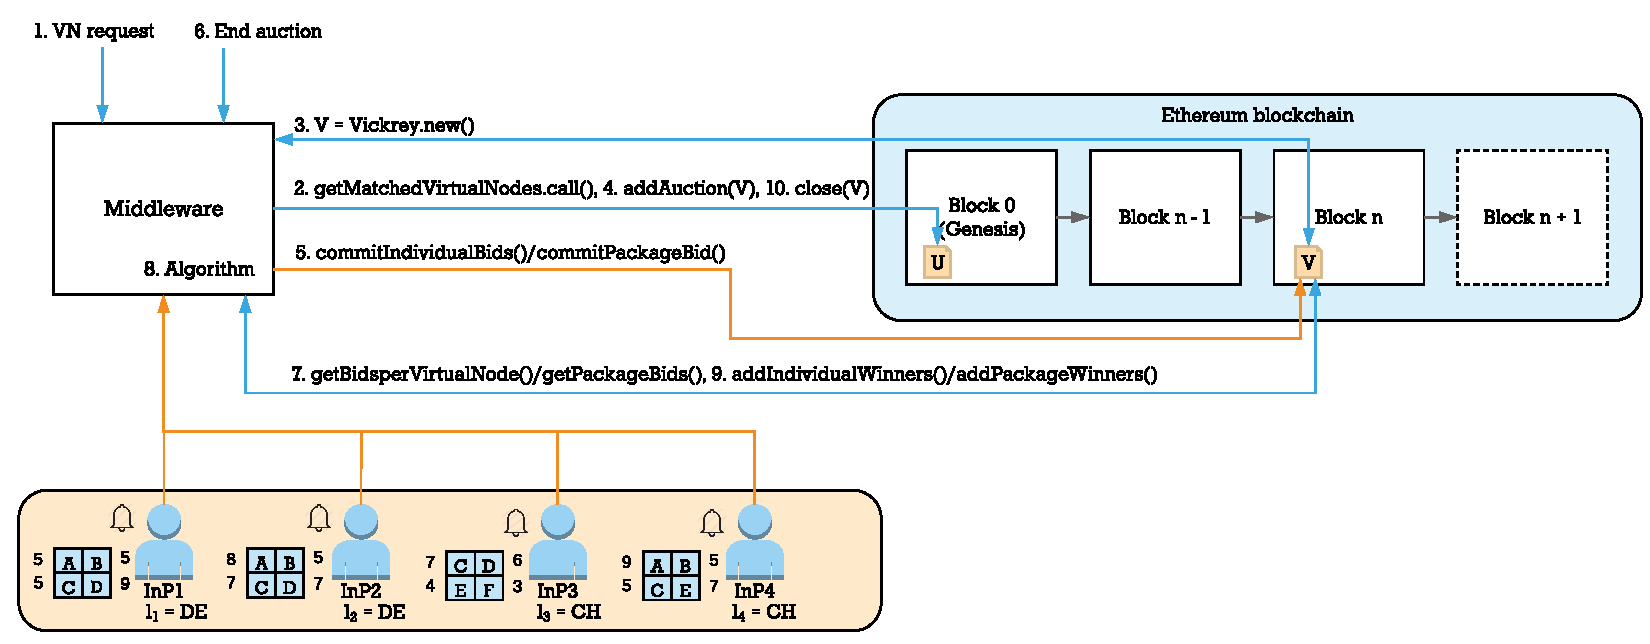
\includegraphics[width=1\linewidth]{gfx/implementation_workflow}    
  	\caption{Virtual network request workflow and system components interaction.}
  	\label{fig:implementationWorkflow}
\end{figure}

\section{Summary}

In this chapter, we have presented the implementation of a VNE system under limited information disclosure. First, the design decisions and environment selected for our approach, which consists of a web application connected to an Ethereum blockchain through a middleware, has been defined. Subsequently, we have further detailed the content of the two fundamental contracts (\textit{Users} and \textit{Vickrey}) used, which facilitates the integration of the defined VN partitioning algorithm into the blockchain. In addition, to exclude smart contracts directly interacting with the external world (users), an authentication system that improves the system's security has been developed. Lastly, we have specified the interaction between our system components during the virtual network partitioning process.

Nevertheless, since the defined system is experimental and still in its early phases, several constraints and improvements are already deducted. Therefore, an evaluation of the different participating components to better reflect and examine the system functionalities is required. In particular, our defined VN partitioning algorithm must be analyzed, together with the blockchain specifications that enhance the system's performance.


%*****************************************
\chapter{Evaluation}
\label{ch:evaluation}
%*****************************************

In this chapter, we evaluate the efficiency of the previously presented brokerless VNE system, which uses the blockchain technology to improve the multi-provider VN embedding throughput under the limited information disclosure scenario. First, we present the evaluation setup, which illustrates the architecture used and describes the substrate and virtual network topologies. In addition, in this section, we introduce a pricing model used for the InPs to dynamically quote their services, and a consensus algorithm, which enhances the standard PoW transmission time in private blockchains while maintaining fairness between the mining nodes. Afterwards, we define the goals and metrics used for characterizing the performance, costs and fairness of the system. Lastly, we will examine and interpret the results of our evaluation.

\section{Evaluation Setup}

Our evaluation is carried out on a single computer with four Intel Core i7-7500U CPU at 2.70 GHz and 16 GB of main memory, using the middleware and back-end components from the prototype described in the implementation chapter. Figure \ref{fig:ev_scenario} depicts the architecture of the evaluation set up, which consists of a middleware that sends the corresponding transactions to the blockchain, through different mining nodes. In this setting, if one node cannot serve the transaction, i.e. it is not available, the request will be sent to the following node to ensure the system functionality.

Moreover, since our system is formed by a hybrid blockchain, multiple nodes (InPs) maintain and serve the infrastructure. In this scenario, we have adjusted the number of available mining nodes ranging from one to five depending on the aim of the test, because this amount of nodes is sufficient to flawlessly compare the different blockchain throughputs. Thus, these mining nodes are set up in different ports from a single machine, each pointing to the same genesis file. In a real world, these nodes will be controlled independently by different firms which cooperate to regulate and ensure the application performance.

\begin{figure}[bth]
	\centering
	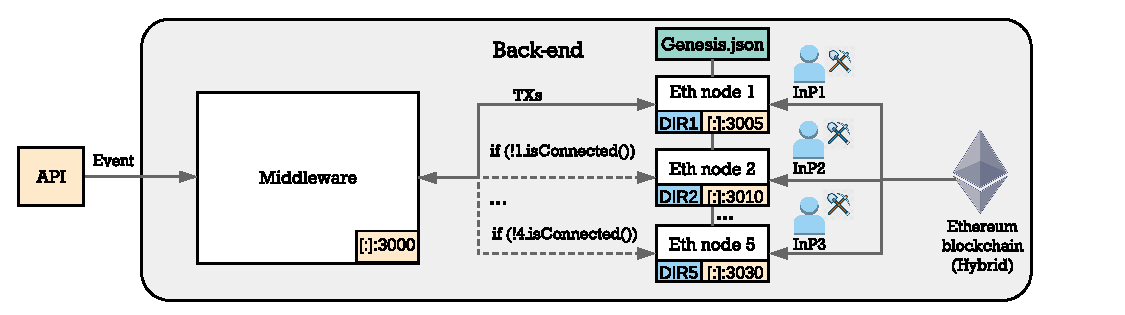
\includegraphics[width=1\linewidth]{gfx/Evaluation_scenario}    
  	\caption{Architecture of the evaluation set up.}
  	\label{fig:ev_scenario}
\end{figure}

In the following, we discuss the substrate network and virtual network request topologies, along with the parameters used in our evaluation. Note that, the values assigned for these parameters have been selected in order to illustrate the subsequent evaluation metrics (section \ref{metrics}).

\begin{itemize}
 \item \textbf{Substrate network:} To simulate a real scenario, we have generated a substrate network based on the network topology from the GÉANT\footnote{\url{https://www.geant.org/}} backbone, which interconnects the National Research and Education Networks (NRENs) across Europe. We have used this model since it is formed by already known non-commercial research and education networks, which do not reveal confidential data. The European NREN dataset model is downloaded from the Internet Topology Zoo \citep{zoo}, which is a project that collects data network topologies derived from publicly available records.

Furthermore, since our evaluation scenario must contain different InPs competing for embedding virtual nodes in diverse locations, we have tailored the European NREN dataset model and their interconnections to fulfill our requirements. Figure \ref{fig:ev_top_a} shows that our substrate network contains nodes located in ten different European countries (yellow nodes), in which InPs possess peering nodes (white nodes). These peering nodes are formed from 3 to 5 resource types (blue boxes), whose availability and costs are, as stated throughout the thesis, not broadcasted. In addition, each node contains a maximum capacity $\mu^{s}_{max}$, i.e. a maximum resource utilization, to identify if the InP can serve incoming VN requests in the selected node.

Apart from those parameters, we need reference costs for every resource type, in order to perform the service negotiation between SPs and InPs. For this reason, we have researched the pricing models and costs, provided by different cloud providers. In particular, Amazon EC2 \citep{amazonEC2} offers a broad selection of instance types along with the corresponding on-demand prices. These instances contain hourly prices per computing capacity, which exactly meets our requirements. Thus, we have extracted the average of the minimum and maximum hourly unitary costs per resource type $\sigma_s$ in the European region, to obtain real values for our presented evaluation scenario.  Specifically, our $\{A, B, C, D, E\}$ node types correspond to the general purpose, compute optimized, memory optimized, accelerated computing and storage optimized Amazon EC2 instance types. The mentioned evaluation parameters for the substrate network are summarized in the left part of Table \ref{tab:evparams}.

\begin{figure}[bth]
	\myfloatalign
	\subfloat[European NREN topology \citep{zoo}.]
	{\label{fig:ev_top_a}%
	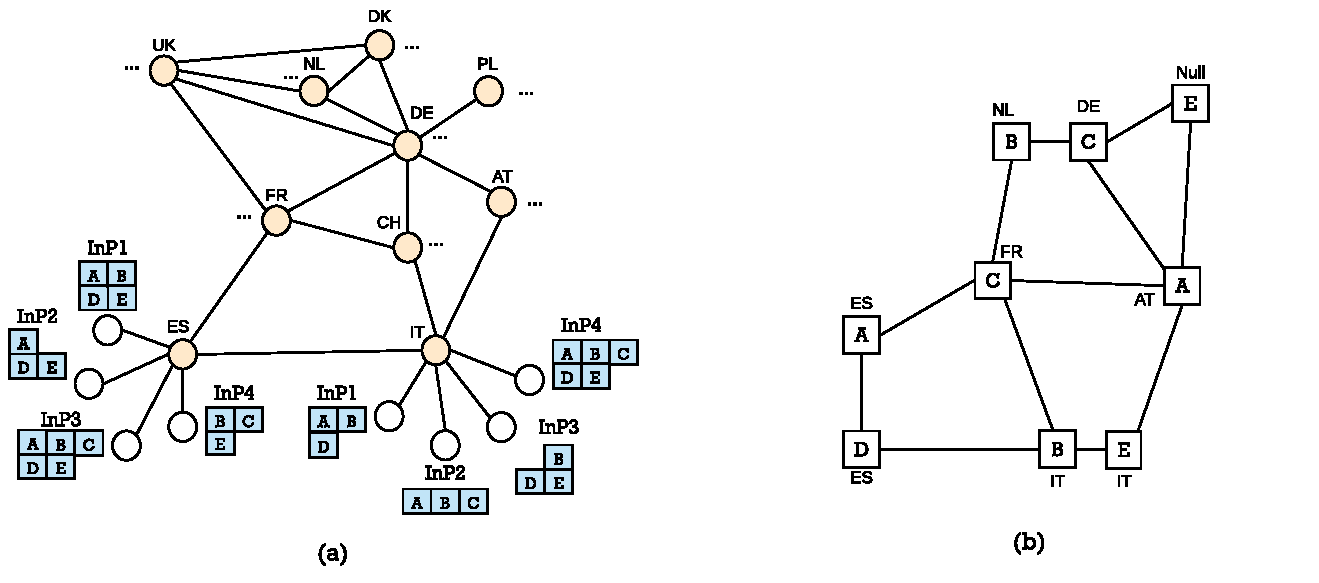
\includegraphics[width=0.48\linewidth]{gfx/Evaluation_topologies}} \quad
	\subfloat[Example of a virtual network request.]
	{\label{fig:ev_top_b}%
	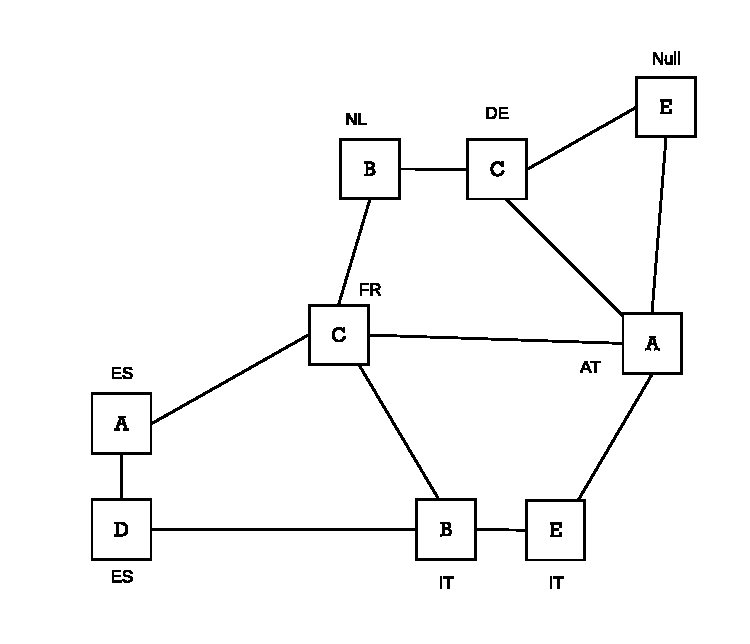
\includegraphics[width=0.48\linewidth]{gfx/Ev_vnr}} \\
	\caption{(a) The evaluation topologies are sampled as subgraphs from the European NREN topology \citep{zoo}. (b) Example of a virtual network request with node types $\{A, B, C, D, E\}$ and locations $\{DE, CH, ...\}$ }
	\label{fig:ev_top}
\end{figure}

\item \textbf{Virtual network request:} A VN request is composed of a set of virtual nodes and the corresponding virtual links. A virtual network request example is depicted in Figure \ref{fig:ev_top_b}. Each virtual node contains exactly the same locations of the substrate network, plus a null one used for embedding the resource type in any location. In addition, the virtual node computing demand $d_i$ and the bandwidth demand $d_{ij}$ are also given from a uniform distribution. In a real world, the bandwidth demand between the virtual nodes is typically given by a traffic matrix. However, note that in section \ref{vickrey}, we have stated that intra-link costs within an InP are negligible and that the inter-links must be roughly estimated by the InPs, due to the lack of information of the other InP's substrate topologies. For simplicity, in this chapter, the inter-links have fixed unitary costs and these are added after partitioning rather than during the bidding process. In other words, if two virtual nodes are embedded to the same InP, no link cost will be added. Nevertheless, if two nodes are contained into two different providers, then the link cost $\beta_{s^{*}}(L_{ij})$ is given by Equation \ref{eq:ev_linkCosts} (derived from Equation \ref{eq:virtualNodeCost}), where $c$ is a constant corresponding to the fixed unitary cost.

\end{itemize}

  \begin{equation} \label{eq:ev_linkCosts}
	\beta_{s^{*}}(L_{ij}) = c \times d_{ij} \qquad i,j \in N^R, \ \exists d_{ij} \neq \infty : \ i \neq j
  \end{equation}

Furthermore, we model the VN requests events through a periodic arrival process with rate $\lambda$. Regarding the lifetime of the VN requests, we fixed those to $L_1 = 10s$ and $L_2 = 25s$. The reason for using periodic arrival rates and fixed lifetimes rather than, for example, Poisson processes and arbitrary lifetimes, is to better study and illustrate the effect of the resource consumption in a non-optimum scenario. The evaluation parameters for the VN requests are summarized in the right part of Table \ref{tab:evparams}.

\begin{table}[bth]
	\myfloatalign \footnotesize
	%18 columns
	\begin{tabularx}{\textwidth}{p{4.5cm}p{3.5cm}|p{4cm}p{4cm}}
	 	\textbf{Substrate Network} && \textbf{Virtual Network Request} \\
		\hline
		InPs & 3 to 7 & Virtual nodes & uniform distrib. [5,10] \\
		Peering node locations & \{ES, FR, IT, CH, DE, AT, PL, NL, DK, UK\} & Virtual node locations & \{ES, FR, IT, CH, DE, AT, PL, NL, DK, UK, NULL\}  \\
		Peering nodes per InP & 10 (1 per location) & Computing demand $d_i$ & uniform distrib. [1,3] \\
		Node types & $\{A, B, C, D, E\}$ & Virtual node types & $\{A, B, C, D, E\}$ \\
		Node types per peering node & uniform distrib. [3,5]  & Bandwidth demand $d_{ij}$ & uniform distrib. [1,10] \\
		Node capacity $\mu^{s}_{max}$ & uniform distrib. [5,100] & Arrival rate $\lambda$ & 1 to 5 requests per second \\
		Unitary cost per node type $\sigma_s$ & uniform distrib. [10,12] & Lifetimes $L_1$ and $L_2$ & 10s and 25s respectively
	\end{tabularx}
	\caption{Evaluation parameters: Substrate network and virtual network request.}
	\label{tab:evparams}
\end{table} 

\subsection{Pricing Model} \label{pricing model}

In section \ref{vickrey}, we have discussed that our approach encourages users to apply dynamic pricing models for network virtualization. In dynamic pricing, there are many strategies to set flexible service costs based on current market demands. In this chapter, we will adapt the demand and supply labels to match our scenario. In particular, the first corresponds to the computing demand $d_i$ for a resource type, and the second to the resource utilization $\mu_s$ in the substrate node maintaining the service.

In contrast to the demand and supply concept, in our evaluation, the capacity does not increase according to the demand, since the resources have fixed maximum capacities $\mu^{s}_{max}$. Thus, the costs will be given according to the current resource utilization, which is based on the residual capacities. Figure \ref{fig:pricing_model} depicts an example of the dynamic cost per hour $\alpha^{h}_{s^{*}}(N_i)$ for the resource type C. From this chart, we can observe how the price gradually increases as the resource is utilized. In this case, the probability of embedding the virtual node is lower, and hence, the resource will wait to embed further VN requests until the node is more released. Equations \ref{eq:ev_price_model} and \ref{eq:ev_resource_uti} (derived from Equation \ref{eq:virtualNodeCost}) reflect the mentioned behaviour, where $\sigma_s$, $\mu_s$, $\mu^{s}_u$ and $\mu^{s}_{max}$ are the unitary cost, resource utilization, used capacity and maximum capacity respectively. In the equations below, note also that the dynamic price per hour $\alpha^{h}_{s^{*}}(N_i)$ is multiplied for the lifetime $L$ of the virtual network request. In case the lifetime $L$ is less than one hour, then the unitary cost $\sigma_s$ must be adapted accordingly.

  \begin{equation} \label{eq:ev_price_model}
	 \alpha_{s^{*}}(N_i) = \alpha^{h}_{s^{*}}(N_i) \times L =  (\sigma_s + \frac{\mu_s}{1 - \mu_s}) \times L \qquad \mu_s \in [0, 1], \ N_i \in N^R 
  \end{equation}
    \begin{equation} \label{eq:ev_resource_uti}
  \qquad \mu_s = \frac{\mu^{s}_u + d_i}{\mu^{s}_{max}} \qquad \mu^{s}_{max} \in [5,100], \ \mu_u \in [0, \mu^{s}_{max}] , \ d_i \in [1, 3]   
  \end{equation}

Therefore, thanks to the presented algorithm, the InPs define their product costs regarding current demands and resources utilization, which provides real-time and on-demand values. These costs are further used to quote prices for the requested virtual node while taking into account the desired profit margins. In future research, this cost estimation can be performed based on many other parameters, which will enable InPs to have a better market positioning.

\begin{figure}[bth]
	\centering
	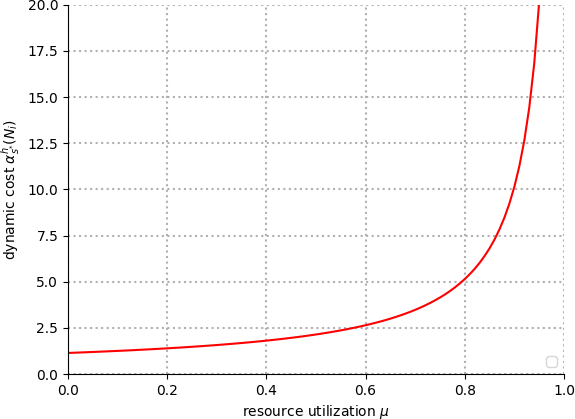
\includegraphics[scale=0.66]{gfx/pricing_model.png}    
  	\caption{Our defined pricing model where dynamic costs increase as more resources are utilized. This is an example for resource type C.}
  	\label{fig:pricing_model}
\end{figure}

\subsection{Proof of Elapsed Time} \label{poet}

At the beginning of chapter \ref{ch:design}, we have discussed the different blockchain types, in order to select the most suitable type for our application: \textbf{the hybrid/consortium blockchain}. In addition, it is obvious that depending on the blockchain type and the desired functionality, different consensus mechanisms need to be used to fulfill the application requirements. For instance, the Ethereum main network uses the \textit{Proof-of-Work} consensus algorithm, which provides fairness between a large number of unknown users, granting them with equal mining probabilities. Nevertheless, since miners need to solve hard cryptographic puzzles to add a new block on the blockchain, this consensus model provides a high energy consumption and slow throughput, which is obviously not an appropriate solution for private blockchains.

For this reason, after examining consensus mechanisms that provide high transaction rates in a scalable and untrusted model, we choose the \textbf{Proof of Elapsed Time (PoET)} protocol. Other consensus algorithms, such as Proof-of-Stake, Byzantine Fault Tolerance or Proof-of-Authority \citep{baliga2017understanding}, have also been investigated. However, the first two were excluded due to the integration complexity into our current Ethereum platform and the third since it sacrifices the trust of our system (not hybrid).

The Proof of Elapsed Time consensus mechanism is used in the Hyperledger Sawtooth project \citep{sawtooth}, designed by Intel. PoET is a lottery based consensus, where the next miner (also called leader) is randomly selected. The workflow is simple: First, each mining node waits a random time (sleep). Afterwards the node with the shortest wait time, wakes up and commits the next block. Finally, the other mining nodes are notified. Here there is an issue of trust. The random sleeping time generation process needs to be the same everywhere. However, the Hyperledger Sawtooth project makes this verifiable by relying on specialized hardware, in particular, on the Intel’s Software Guard Extensions (SGX) \citep{sgx}. Through this trusted environment, the participants are supplied with fair waiting times. Nevertheless, in our scenario, we will assume that there are no malicious nodes manipulating these waiting times. To summarize, we will tailor the idea of PoET to fit in our Ethereum platform.
 
\section{Goals and Metrics}  \label{metrics}

Due to the lack of previous work on multi-provider VNE using the blockchain technology, the main goals of this chapter, are to check the feasibility of the introduced solution and to demonstrate its practical potential. Thus, we set up the previous environment (Figure \ref{fig:ev_scenario}) based on the architecture presented in \ref{architecture}, to explore the benefits and implications of the proposed system.

Moreover, to study the behavior and performance of our approach, each InP makes use of the previously introduced pricing model (section \ref{pricing model}), with homogenous prices. Apart from the real cost of the asset, note that each InP defines his own profit margins $\gamma_n(N_i),\gamma_n(G)$, to perform the bid. Therefore, we will also examine how the deviations in these values affect the final outcome of the VN partitioning.

On the other hand, another fundamental factor for the throughput of our system is the different blockchain specifications. From these properties, one of the key elements that directly influence the functionality is the consensus mechanism employed by the mining nodes. For this reason, we first investigate why the \textit{Proof-of-Work (PoW)} protocol hinders the system performance and check if altering the block difficulty optimizes the results. In addition, we also inspect whether the aforementioned \textit{Proof of Elapsed Time (PoET)} protocol enhances PoW while maintaining fairness between the mining nodes.

Following these definitions, we further summarize the metrics used in our study:

 \begin{itemize}
\item \textbf{Acceptance rate}: Based on our approach and the proposed pricing model, we examine the VN embedding efficiency through the acceptance rate. This VN acceptance rate is the percentage of embedded virtual nodes from the total incoming VN requests. Nevertheless, these values are significantly influenced by many circumstances. Between these, we demonstrate how the following parameters alter the performance: (i) the virtual network request lifetime $L$, (ii) the number of participating InPs $I_p$ and (iii) the VN requests arrival rate $\lambda$.

\item \textbf{Bidding strategy}: The bidding strategies are evaluated based on how the profit margins $\gamma_n(N_i),\gamma_n(G)$ employed by the different InPs, produce significant revenues on certain scenarios. 

\item \textbf{Blockchain performance}: In this thesis, the blockchain performance will be verified basically in terms of the block generation time (mining) and the number of forks. The former, is the more accurate manner to calculate the speed of the transactions since each block contains many transactions. The latter: once the block generation time decreases, the number of new blocks solutions increases, which as a consequence creates forks on the blockchain. Another parameter that also steps up the number of forks is the network latency. Nevertheless, since our mining nodes are on a single machine and these latency values are not large in a real world, we will neglect the network latency between our mining nodes.
\item \textbf{Mining fairness}: We consider our system fairness regarding the mining nodes contribution into the blockchain growth, i.e. the number of blocks that each node mines. Since our approach corresponds to a hybrid blockchain, where each InP coordinates and ensures the system's functionality, the effort on mining blocks must be equally shared between the blockchain nodes. Thus, in a fair system, each node roughly mine the same number of blocks.
 \end{itemize}

Furthermore, it is important to note that thanks to blockchain and smart contracts flexibility, the results obtained thereupon are not definitive findings, since they can always be improved by upcoming investigations.

\section{Evaluation Results}

In this section, we present the evaluation results of the Vickrey auction model based on a demand-resource pricing model, and using the Ethereum platform in a private network. Through the aforementioned metrics and parameters, we provide different results for various scenarios during the evaluation process. These parameters are summarized in Table \ref{tab:ev_notations}.

\begin{table}[htbp]
	\myfloatalign \footnotesize
	\begin{tabular}{m{2cm} m{13.5cm}}
		\textbf{Symbol} & \textbf{Description}\\ 
		\hline
		$\sigma_s$ & unitary cost for a resource type in substrate node $N_s^{*}$  \\
		$\mu_s$ & variable $\in [0,1]$ expressing the resource utilization in substrate node $N_s^{*}$ \\
		$\mu^{s}_{max}$ & variable $\in [5,100]$ expressing the maximum capacity of a resource type in substrate node $N_s^{*}$ \\
		$\mu^{s}_u$ & variable $\in [0,\mu_{max}]$ expressing the used capacity of a resource type in substrate node $N_s^{*}$ \\
		$\alpha^{h}_{s^{*}}(N^R)$ & dynamic hourly unitary cost for virtual network request $N^{R}$ \\
		$\varphi$ & acceptance rate $\varphi \in [0,1]$ \\
		$I_p$ & participating InPs \\
		$\lambda$ & virtual network request arrival rate (number of requests in 5s) \\
		$L$ & virtual network lifetime \\
		$B_m$ & mined block \\
		$t_B$ & block generation time \\
		$D_B$ & block difficulty \\
		$D_{B_p}$ & parent block $B_p$ difficulty \\
		$f_B$ & number of forks in $B$ blocks \\
		$w_n$ & PoET window time of mining node $n$ \\
		$x_i$ & miner IDs \\
		\hline
	\end{tabular}
	\caption{Evaluation notations}
	\label{tab:ev_notations}
\end{table}

\subsection{Acceptance Rate and Bidding Strategy}

Initially, to measure the acceptance rate of our model under different conditions, we first study the influence of the VNR lifetime $L$. The reason to prove this is that the VNR lifetime has most probably a significant impact on the performance, as our defined pricing model (section \ref{pricing model}) is directly linked to the resource utilization.

Therefore, we have defined a scenario where three participating InPs ($I_p$) with zero profit margins ($\gamma_n(N_i),\gamma_n(G) = 0$) embed 100 VNR across 200 runs. In the first half of the runs, these requests have a short lifetime $L_1 = 5s$. Then, to compare the outcome with a larger lifetime, a second lifetime $L_2=20s$ has been set for the remaining runs. In addition, these requests are sent periodically every second, i.e. with arrival time $\lambda = 5$.

Figure \ref{fig:acceptance_rate} illustrates the average acceptance rates $\varphi$ with CI=0.95, when the lifetimes $L_1$ and $L_2$ are applied. As expected, this value is higher for $L_1$ inasmuch as shorter lifetimes ($L_1 < L_2$) utilize the resources for a less period, and consequently, the nodes are earlier released. More specifically, first, the acceptance rate decreases for both cases as the resources are gradually filled, which hampers the embedding of the following VNRs. Afterwards, we contemplate that both lifetimes reach steady states as the number of VNR grows. This is because the lifetime of the first incoming VNR expires, which reduce the nodes used capacities $\mu^s_u$. Since this cycle is repeated over the time, it produces the named steady state. In particular, $L_1$ and $L_2$ start to experience this phenomenon around 10s and 25s respectively, which exactly corresponds to the lifetime of our requests.

\begin{figure}[bth]
	\centering
	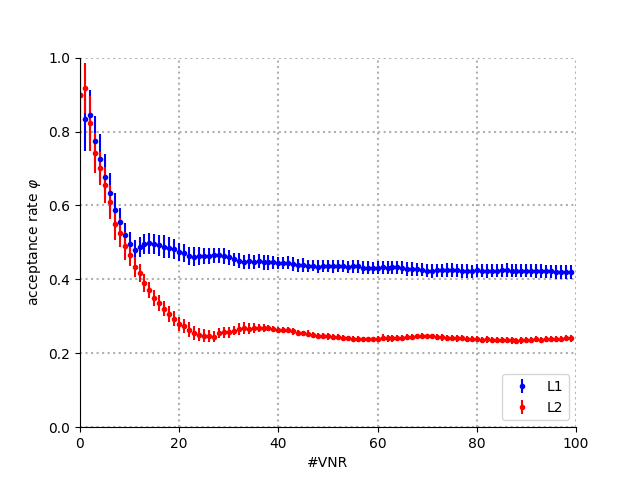
\includegraphics[scale=0.65]{gfx/ev_acceptance_rate.png}    
  	\caption{Average acceptance rate $\varphi \in [0,1]$ with CI = 0.95 describing the fraction of requests accepted. After a transient phase the request acceptance rate is dependent on the request lifetime $L$.}
  	\label{fig:acceptance_rate}
\end{figure}

\begin{figure}[h!]
	\centering
	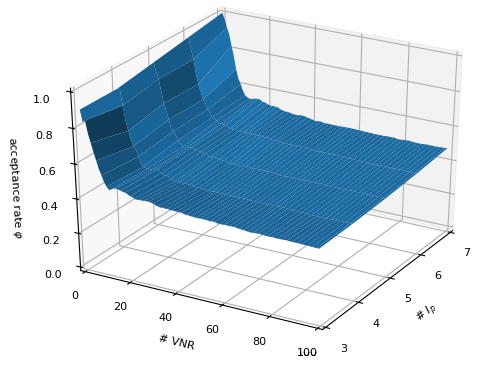
\includegraphics[scale=0.9]{gfx/ev_acceptance_rate3D.png}    
  	\caption{Average acceptance rate $\varphi \in [0,1]$ for $L = 5s$ and $\lambda = 5$, describing the fraction of requests accepted for a different number of infrastructure providers $I_p =[3,4,5,6,7]$. The acceptance rate is slightly higher as $I_p$ increases.}
  	\label{fig:acceptance_rate_3D}
\end{figure}

In Figure \ref{fig:acceptance_rate}, we have seen that at the beginning, a high volume of requests in a short period, cause that the acceptance rate scales down, since the resource utilization augment. For this reason, we need to investigate how the throughput is enhanced, when there are more resources, or in other words, as the number of $I_p$ increases. Thus, we will repeat the experiment again, now in presence of 3 to 7 InPs, using $\lambda = 5$ and $L_1$. Despite the fact that with large lifetimes $L_2$ the differences would have been obviously higher, in this trial, we have applied a lifetime $L_1$, in order to observe whether the acceptance rate also varies for small lifetimes. Figure \ref{fig:acceptance_rate_3D} illustrates the average acceptance rates $\varphi$ with 3 to 7 $I_p$.

\begin{figure}[bth]
	\centering
	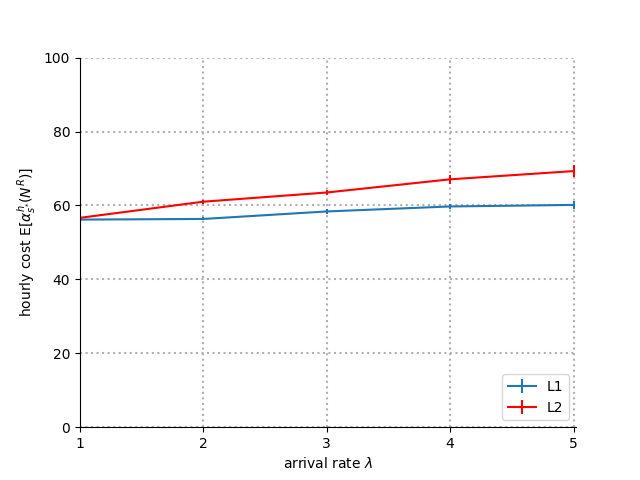
\includegraphics[scale=0.68]{gfx/ev_pricing.png}    
  	\caption{Impact of the periodic arrival process rate $\lambda$ on the average hourly costs. A higher request arrival rate causes a cost increase due to a higher resource utilization.} 
  	\label{fig:pricing}
\end{figure}

Firstly, we observe that with $I_p = 3$ the acceptance rate $\varphi$ exactly matches our introduced Figure \ref{fig:acceptance_rate}. Nevertheless, the interesting point is once $I_p$ has a greater value. In this case, we notice that the initial acceptance rate is larger since the number of free resources is bigger. Besides, we also contemplate the slight slope reflected during the VNR, although Figure \ref{fig:acceptance_rate_3D} provides no statistical evidence of a significant slope for a determined number of $I_p$. Thus, we can assert that for $L_1$ the acceptance rate $\varphi$ slightly improves initially, even though in the end, the steady-state difference is not steep. However, we can deduce that for larger lifetimes the slope variations will be more meaningful.

On the other hand, we have above-mentioned that our costs are directly linked to the resource utilization. For this reason, an analysis of our proposed pricing model is extremely required. In addition, in the following test, we also investigate the arrival rate $\lambda$ footprint on the VNR costs, tailoring these values from one to five, i.e. from one to five requests every 5s. These values are chosen with regard to five seconds, because the minimum processing time for one request in our system is approximately 1s, meaning that $\lambda = 5$ corresponds to this minimum (1 req/s).

Figure \ref{fig:pricing}, depicts the average hourly costs for the requested virtual nodes $N^R$ with lifetimes $L_1$ and $L_2$, towards the different arrival rates. Note that this value corresponds to the hourly cost $\alpha^{h}_{s^{*}}(N^R)$ rather than the final $ \alpha_{s^{*}}(N^R) = \alpha^{h}_{s^{*}}(N^R) \times L$. In this manner, the impact of the different arrival rates and lifetimes is best reflected, since the cost difference is directly proportional to the resource utilization. Besides that, to better precise the mean costs in a graph, we have reduced the randomness of $N^R$, fixing the number of VNRs to 5 rather than applying a uniform distrib. [5,10]. Thus, since in Table \ref{tab:evparams}, we have defined that the nodes unitary costs $\sigma_s$ values are around 10 and 12, and the number of $N^R = 5$, the minimum costs of $\alpha^{h}_{s^{*}}(N^R)$ start roughly at 50.

In case of small arrival rates ($\lambda = 1$), as the resources are less utilized, then the Equation \ref{eq:ev_price_model} results in $\alpha^{h}_{s^{*}} \approx \sigma_s$, and hence, to 50 independently of the applied lifetimes. However, once the arrival rate value increases, the deviations from $L_1$ to $L_2$ are higher. The main reason is that the second term of the Equation \ref{eq:ev_price_model}, tends to infinity when the resources are occupied, which occurs frequently by large lifetimes. For instance, when $\lambda = 5$, the difference between $L_1$ and $L_2$ on the average cost is approximately $21\%$.

In the previous experiments, we have evaluated the acceptance rate $\varphi$ regarding the lifetimes $L_1$ and $L_2$, and different $I_p$. In addition, we have studied how the costs are altered with different arrival rates $\lambda$. 

Nevertheless, we have considered so far that the InPs apply zero profit margins ($\gamma_n(N_i), \gamma_n(G) = 0$), which indicates that the bidder strategies need to be further assessed. Thus, we have set up a similar scenario with the same arrival rates $\lambda$, lifetimes $L_1$ and $L_2$ and $I_p = 3$, where each InP has individual and package profits $\gamma_1 = 0.1, \gamma_2 = 0.2, \gamma_3 = 0.4$ respectively. 

Moreover, to prevent that InPs use immense profit margins, we have established a VN upper bound cost $u_G = 80$, which is a slight increment of the maximum cost reached in Figure \ref{fig:pricing}. Figure \ref{fig:winners} depicts the average fraction of requests assigned to each InP. To remark the differences, in this plot, we have divided the results for $L_1$ and $L_2$, which corresponds to Figures \ref{fig:winners1} and \ref{fig:winners2} respectively. In the first, we observe that for low arrival rates the values between the $I_p$ are completely different because the resources are not yet fully occupied. Hence, the InP with lower profit margins, in this case, InP1 embeds most of the VNR. In contrast, for larger $\lambda$, the second InP, since the InP1 resources are utilized, start to gradually increase the number of embedded VNRs. Finally, InP3 embeds the remaining VNR, although this amount is not significant since the other InPs can still deal with the requests.

Meanwhile, when the VNR contain larger lifetimes $L_2$ (Figure \ref{fig:winners2}), the denouement is more weighted. From the beginning, since the InP's resources are largely populated, the incoming requests need to be served by other InPs. Naturally, first the InPs with lower profit margins handle the petitions. However, as the number of resources is not sufficient, InPs with bigger profits start to embed a meaningful fraction of them.

To summarize, in this section, we have studied the acceptance rate based on several parameters, and an example outcome for InPs with different bidding strategies has been introduced. After examining these results, we first conclude that a huge number of available resources, i.e. multiple InPs, are essential for achieving great acceptances rates. This can be contemplated, after disrupting the system performance through different arrival rates $\lambda$ and lifetimes $L_1$ and $L_2$, which detects the changing behaviors in the worst case scenarios. In addition, thanks to the bidding strategy experiment, we have observed that InPs with high-profit margins also embed VNR under certain conditions (large lifetimes $L$ and arrival rates $\lambda$). For this reason, we reinforce the idea introduced during this thesis, which states that a well-executed market research can be translated with higher revenues, and thereby, to a better market positioning.

\begin{figure}[t]
	\myfloatalign
	\subfloat[lifetime $L_1$ = 10s.]
	{\label{fig:winners1}
	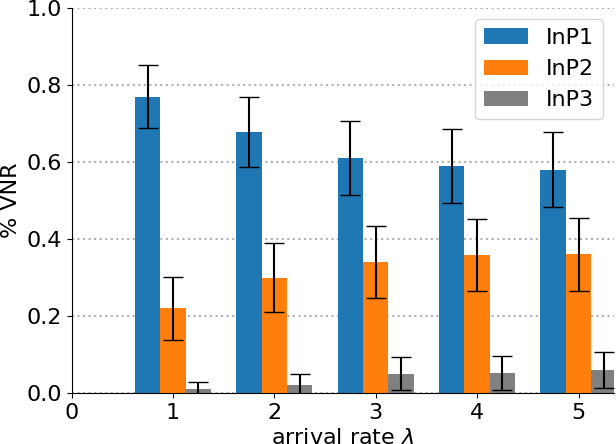
\includegraphics[width=0.48\linewidth]{gfx/ev_winners_L1.png}} \quad
	\subfloat[lifetime $L_2$ = 25s.]
		{\label{fig:winners2}
	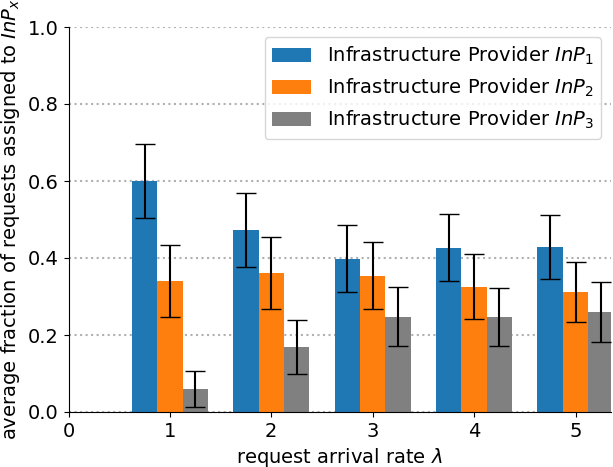
\includegraphics[width=0.48\linewidth]{gfx/ev_winners_L2.png}} \\
	\caption{Average fraction of VN requests assigned to each InP with different arrival rates $\lambda$ and lifetimes $L_1 < L_2$. The InPs are heteregenous with different profit margins $\gamma_1 = 0.1, \gamma_2 = 0.2, \gamma_3 = 0.4$. With large lifetimes $L$ and arrival rates $\lambda$, InPs with higher profit margins start to embed more virtual network requests.}
	\label{fig:winners}
\end{figure}


\subsection{Blockchain Performance and Mining Fairness} \label{resultsBlock}

In the following, we first study how the Proof of Work (PoW) specifies the block generation time. This value is related to the time that a miner needs to find a valid block header, whose cryptographic hash is less than $\frac{2^{224}}{d}$, where $d$ is the block difficulty (Equation \ref{eq:proofOfWork}). Thus, the block difficulty $D_B$, which changes per each block following a difficulty adjustment algorithm, fundamentally provides the block generation time. In Ethereum, this is given by Equation \ref{eq:pow}, where $D_{B_p}, T_p$ and $T_b$ are the parent block difficulty, parent block timestamp and current block timestamp respectively.

\begin{equation} \label{eq:pow}
 D_B = D_{B_p} + \frac{D_{B_p}}{2048 \times \text{max}(1-(\frac{T_b - T_p}{10}), -99)} + 2^{(\frac{B}{100000} - \ 2)} 
  \end{equation}

The Equation \ref{eq:pow} can be divided into two parts. The left part provides the difficulty adjustment, which increases or decreases depending on the time difference between the current block timestamp $T_b$ and the parent block timestamp $T_p$. In particular, when $T_b - T_p < 10s$, the difficulty is adjusted upwards by $D_{B_p} - \frac{D_{B_p}}{2048 \times 1}$. Converserly, for $10s <= T_b - T_p < 20s$ the difficulty remains unaltered and for $T_b - T_p > 20s$, it is adjusted downwards from $D_{B_p} - \frac{D_{B_p}}{2048 \times -1}$ until $D_{B_p} - \frac{D_{B_p}}{2048 \times -99}$. Regarding the right part of Equation \ref{eq:pow}, also called the difficulty bomb, it exponentially increases the difficulty every 100000 blocks. The aim is to cause that mining a block is harder over the time, which will create less blocks, and hence, less mining rewards. In addition, this value is also intended for switching from PoW to Proof-of-Stake (PoS) at some point in the future.

Despite being in a private network typically implies fewer transactions than in a public network, we must bear in mind that every time that the state of a smart contract is changed, it is considered as a transaction. Since this action frequently occurs in a private environment, and even if the difficulty is configured with a small value in the genesis block, the increasing difficulty provokes, hence, ending up with undesired mining times (around 12s in the Ethereum main network). For this reason, we claim that using the standard PoW in private networks is not logical, and we must consider other consensus algorithms.

The first approach is to establish an almost negligible difficulty with a fixed value from the beginning. To achieve this, we have modified a file from the open source code of Ethereum that defines the PoW consensus model (go-ethereum-master/consensus/ethash/consensus.go). Specifically, the CalcDifficulty function (line 2 in Listing \ref{lst:tailorPow}) now returns 0x400, which is the hexadecimal value of 1024. Due to the bound divisor of Equation \ref{eq:pow}, in the PoW algorithm, this value cannot be smaller than 2048. For this reason, in this test, we have chosen a value that is a half of this minimum, which already give us huge differences. However, for further evaluations, this value could be set to even a smaller value (also in genesis block), such as big.NewInt(1), although the results will be almost equal.

Furthermore, since a continuous and disproportionate growth of the blockchain is in most cases illogical for private networks, we have preloaded a JavaScript function that restricts the mining only with the presence of transactions (line 6 in Listing \ref{lst:tailorPow}). For instance, miner.start(miningThreads) begins the mining with mining threads being the number of used processor cores, and eth.getBlock("latest").number gets the block number of the latest mined block.
\newline

\begin{lstlisting}[language=JavaScript,caption={Defined functions that specify the block difficulty and the tailored PoW.}, label={lst:tailorPow}]
func (ethash *Ethash) CalcDifficulty(chain consensus.ChainReader, time uint64, parent *types.Header) *big.Int {
    return big.NewInt(0x400)
}

var miningThreads = 1;
function tailoredPow() {
    if (eth.getBlock("pending").transactions.length > 0) {
        txBlock = eth.getBlock("pending").number
        if (eth.mining) return;
        miner.start(miningThreads)
        while (eth.getBlock("latest").number < txBlock) {}
        miner.stop()
    }
    else {
        miner.stop()
    }
   }
\end{lstlisting}

\begin{figure}[bth]
	\myfloatalign
	\subfloat[Proof of Work (PoW).]
    {\label{fig:forks1}
	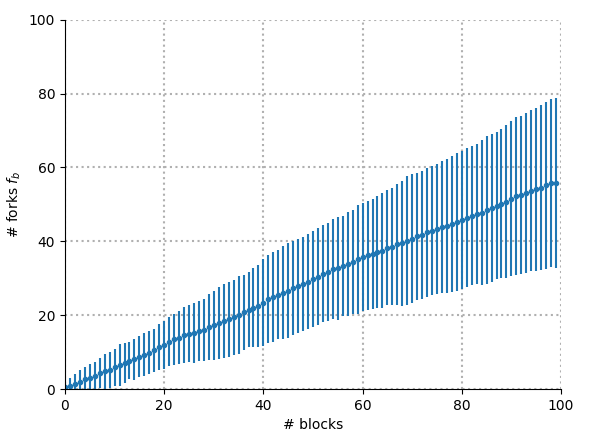
\includegraphics[width=0.48\linewidth]{gfx/ev_forks_pow.png}} \quad
	\subfloat[Proof of Elapsted time (PoET).]
	{\label{fig:forks2}
	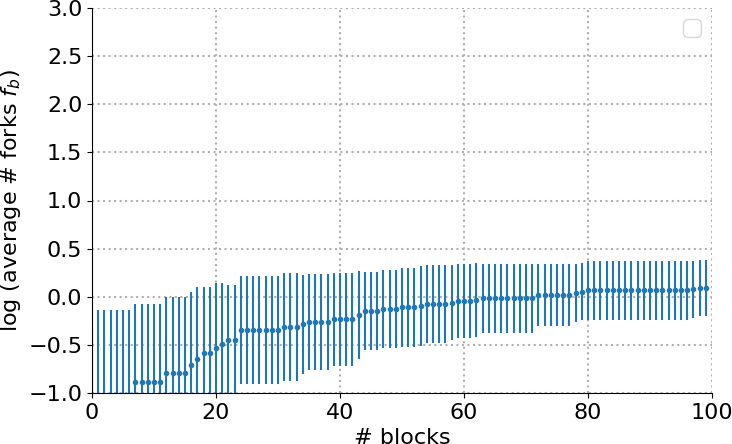
\includegraphics[width=0.48\linewidth]{gfx/ev_forks_poet.png}} \\
	\caption{Number of forks $f_b$ per block with three mining nodes using PoW with tiny difficulty and PoET. Note that the difference depends on the parameter of PoW, i.e. the difficulty. and the parameter of PoET, i.e. the window size $w_n$.}
	\label{fig:forks}
\end{figure}

\begin{figure}[bth]
	\myfloatalign
	\subfloat[Proof of Work (PoW).]
	{\label{fig:fairness1}
	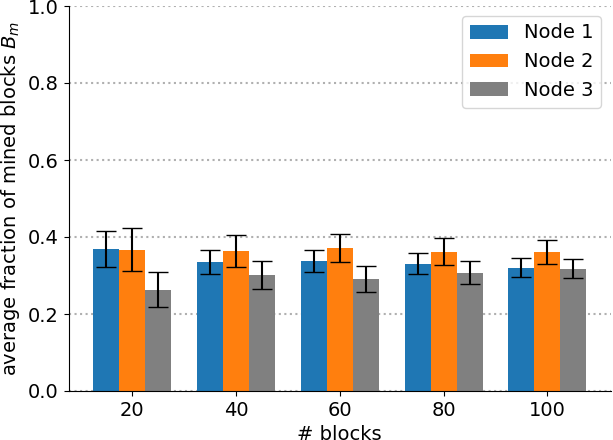
\includegraphics[width=0.48\linewidth]{gfx/ev_fairness_pow.png}} \quad
	\subfloat[Proof of Elapsted time (PoET).]
    {\label{fig:fairness2}	
	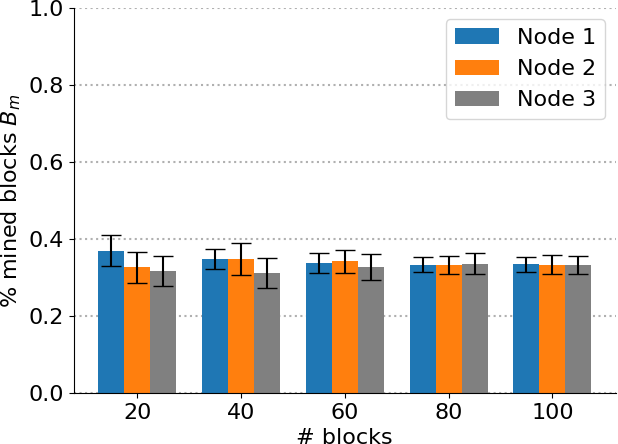
\includegraphics[width=0.48\linewidth]{gfx/ev_fairness_poet.png}} \\
	\caption{Average fraction of mined blocks $B_m$ among three mining nodes using PoW with tiny difficulty and PoET. Using PoET the average fraction converges faster to a fair leader election.}
	\label{fig:fairness}
\end{figure}

In the following, we analyze the blockchain performance of the proposed solution, in terms of block generation time, number of forks and mining fairness. This evaluation is carried out with three mining InPs, defined locally in three different ports (Figure \ref{fig:ev_scenario}).

\begin{itemize}
\item \textbf{Number of forks}: The maximum number of forks for $b$ blocks are $f_b = b \times (n-1)$, where $n$ are the corresponding miners (3 in our test). Figure \ref{fig:forks1}, illustrates the logarithmic average number of forks $f_b$ with CI=95\% along 100 blocks. This value is $\log_{10}(f_b) \in [0,1.75]$, more explicitly from 1 to 56 forks. If we compare the obtained values, with the worst case scenario $f_{100} = 100 \times (3-1) = 200$, this already corresponds to a 28\% of the maximum possible forks with only 3 InPs. This produces a significant amount of misused work, which as in private networks the amount of miners is smaller, can result in important losses on throughput. In addition, it is also important to note that this value will increase as the number of mining peers grows.
\item \textbf{Mining fairness}: In Figure \ref{fig:fairness1}, we contemplate the average fraction of mined blocks $B_m$. Since the system is a modified version of the PoW with almost negligible difficulty, it still conservates the fairness given by the PoW algorithm. This fairness converges faster to a fair leader election, as the number of mined blocks grows, and by contrast, it is more arbitrary in the beginning.
\item \textbf{Block generation time}: Since the difficulty is fixed for all the mined blocks, the block generation time $t_b$ is practically constant $t_b \in [1,2]$. Compared to the standard PoW, the $t_b$ has decreased considerable, which entirely fulfills the requirements of a private blockchain.
 
\end{itemize}

Therefore, the tailored PoW consensus model offers great block generation times while maintaining a fair system. Nevertheless, multiple miners resolve blocks at the same time since the difficulty is extremely low, which directly hinders the system performance with a huge expenditure of resources. Moreover, as having a higher number of mining nodes directly implies extra losses, this causes that the system suffers from scalability. 

For this reason, we introduce a second approach, which implicitly, evaluates the PoET consensus model explained in section \ref{poet}. To prove this, first, we define an identical window time $w_n$ for each of the $n = 3$ mining nodes. In this workflow, only when a new transaction arrives, the mining nodes wait an arbitrary time between 1 or 10 seconds ($w_n \in [1,10]$), before appending a new block. Since in PoET there is no cryptographic work, the block generation time is similar to the waiting period. Hence, the window range must not be too large (slow throughput), and not too short (many forks occurring). This is why a $w_n \in [1,10]$ appears to be a proper starting point. 

The following code, see Listing \ref{lst:PoET}, shows the implemented JavaScript functions. From this, it is important to understand line 7, which is the responsible for calling the function startMining() after waiting an arbitrary time given by the window $w_n$. Once entering the function, if the old txBlock is still equal to the pending block number, then the mining proceeds.
\newline

\begin{lstlisting}[language=JavaScript,caption={Defined functions to apply the Proof of Elapsted Time (PoET) in an Ethereum client.}, label={lst:PoET}]
var timeout_set;
var miningThreads = 1;

function simulatePoET() {
    if (eth.getBlock("pending").transactions.length > 0) {
        if (timeout_set || eth.mining) return;
        var txBlock = eth.getBlock("pending").number;
        timeout = setTimeout(startMining(txBlock), getRandomInt(1000,10000));
    }
    else {
        miner.stop()
    }
}

function startMining(txBlock) {
    if (txBlock === eth.getBlock("pending").number) {
        if (eth.mining) return;
        miner.start(miningThreads);
        while (eth.getBlock("latest").number < txBlock) {}
        miner.stop();
        timeout_set = false;
    }
    else {
        timeout_set = false;
    }
}

function getRandomInt(min, max) {
    var time = Math.floor(Math.random() * (max - min)) + min;
    timeout_set = true;
    return time; //The maximum is exclusive and the minimum is inclusive
}
\end{lstlisting}

Hereafter, we further analyze the PoET algorithm based on the last introduced metrics: 

\begin{itemize}
\item \textbf{Number of forks}: Figure \ref{fig:forks2} depicts the logarithmic number of forks along 100 blocks using the PoET consensus model. At first glance, we can observe a pronounced decrease, using the same three mining nodes. In particular, after 100 blocks, the mean value is around 0.1, which corresponds to 1.25 forks. Compared to the number of $f_b$ using the tailored PoW, now the percentage is only 0.625\% with respect to the maximum, rather than 28\%.
\item \textbf{Mining fairness}: Thanks to the randomness given by the window time $w_n$ and the non-presence of malicious nodes, in this scenario, the miners have equal mining privileges. In Figure \ref{fig:fairness2}, we can contemplate how the mining tasks are successfully distributed since the beginning. Thus, the introduced approach also preserves fairness without the need of solving any cryptographic work.
\item \textbf{Block generation time}: In this case, the block generation time is not given by any complex algorithm. Conversely, the value is directly proportional to the shortest waiting time randomly chosen by the miners. For this reason, we will study the changes on the block time, when the number of mining InPs increases or decreases. In particular, Figure \ref{fig:block_time} illustrates the box plot of the resulting average block times $t_b$ with one to five miners, in comparison to the analytic block times (red dots). Since analytic block times do not include computational periods, these values are smaller than the ones extracted from our application. In case of a one-dimensional model (1 InP), the analytic block times are directly related to the mean values. On the other hand, in a two-dimensional model (2 InPs) this is given by Equation \ref{eq:averageBT}, where $k$ is the maximum value of the window $w_n$. For instance, with 2 InPs and $w_n \in [1,10]$, the block time is $t_b = 3.85s$. Going back to the block time depicted in Figure \ref{fig:block_time}, we observe that once the number of InPs increases, since the probability of obtaining shorter waiting times is higher, the block time is reduced accordingly. Nevertheless, due to the big size of our defined window time, when the number of InPs is small, the block time is too long. For instance, with only one miner the block time is approximately 5.5s, which is a poor throughput as with a single miner no forks can occur. Thus, regarding forks, the presence of more miners creates more forks $f_b$ on the blockchain (not shown in the graph), although in our example, thanks to the wide defined window time $w_n$, this effect is not severe.

  \begin{equation} \label{eq:averageBT}
 E [t_b] = \sum_{i = 1}^{k} \frac{(2k + 1)-2i}{k^2}  
  \end{equation}
  
\end{itemize}

\begin{figure}[bth]
	\centering
	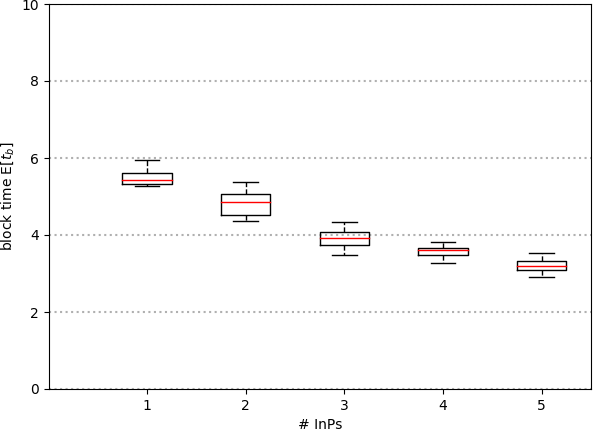
\includegraphics[scale=0.7]{gfx/ev_block_time.png}    
  	\caption{Average block time with different InPs mining and using the PoET consensus protocol. The difference between the analytical model and the real-world measurement is probably due to the overload in block generation (computation) and in the overhead of informing the other mining nodes.}
  	\label{fig:block_time}
\end{figure}
  
  
Therefore, our proposed PoET consensus model maintains fairness on the system. However, since the blockchain time $t_b$ is given now as a function of $w_n$, an approach that defines the window size maintaining fast throughputs and avoiding forks must be investigated. 

In a best case scenario, from a set of windows $w = \{w_1,w_2,...,w_n\}$, the system distributes one window for each miner, being the difference between each window $\Delta w$ greater or equal to the averaged sum of computational times $t_{com}$ in one node ($\Delta w = w_{i+1} - w_i \geq t_{com} $). For instance, imagine a scenario with 3 InPs, $t_{com} = 1$ and window set $w = \{1,2,3\}$, where the last two blocks have been mined by miner 1 and 2 consecutively. Then, for the next block each InP should be supplied with a window that ensures fairness on the system, i.e. $w_1 = 2, w_2 = 3, w_3 = 1$. Despite the optimum window values are simple to identify, the problem lies in the distribution of those, such that decentralization and scalability is preserved. Thus, we immediately discard placing a central node that distributes the window times for each mining node.

On the contrary, we introduce the pseudocode for a decentralized PoET window time distribution, where the last miner distributes the next window periods creating a pair $p$ for each of the $n$ miners. A possible solution to perform the allocation could be writing the pair set in the \textit{extraData} field of each block, before mining it. Then, once each miner receives a notification from the latest mined block, they could pull the window time matching their address.

 \begin{algorithm}
  \caption{Pseudocode for a decentralized window time distribution across multiple mining nodes}
 \label{alg:algorithm2}
  \begin{algorithmic}[1]
  \STATE{$w = \{w_1,w_2,...,w_n\}: \ \Delta w = w_{i+1} - w_i \geq t_{com} $}
  \STATE{$x = \{x_1,x_2,x_j,...,x_n\}$}
  \STATE{$x^{'} = x - \{x_j\}$}
  \STATE{$p = \{p_1,p_2,...,p_n\}$}
  \STATE{$p_n = \{x_j, w_n\}$}
  \FOR{$i=1;\ i < n$}
 	\STATE{$k = rand\{x^{'}\}$}
 	\STATE{$x^{'} = x^{'} - \{k\}$}
 	\STATE{$p_i = \{x_k, w_i\}$}
  \ENDFOR
 \end{algorithmic}
\end{algorithm}

In Algorithm \ref{alg:algorithm2}, $x$ corresponds to a set containing the miner addresses, where $x_j$ is the last miner, i.e. the user executing the algorithm. First, the miner creates a pair $p_n$, which contains his address and the maximum value of the window. Afterwards, a loop process starts, where each miner is matched with a new window time. It is important to note that in this example, the cycle does not utilize any past data regarding miners preceding the last block, although this could be further implemented, keeping track of them by storing their addresses in the memory.

In essence, in this section, we have demonstrated that the consensus model used in a private network directly affects the blockchain throughput. First, we have studied how the block time is derived from the standard PoW used by Ethereum. Since the difficulty has a big impact, we have tried to minimize this value by tailoring the Ethereum PoW. Due to the almost non-existent cryptographic work, this has directly caused that multiple miners create different solutions at the same time (forks). 

For this reason, we have introduced PoET, which has considerably reduced the number of forks while maintaining fairness on the system. Since in this protocol each miner waits an arbitrary time given by the window size, this value has an extremely important role in determining the block time. To study the system behavior, we have first performed our test with $w_n \in [1,10]$, where each miner picks and waits independently a random time inside this range. Nevertheless, as the window time is fixed for all the scenarios, this produces a poor throughput when there is a small number of peers, and several forks when the number of participating nodes is higher. As a consequence, we have presented a possible solution for optimizing these values, by establishing a prior agreement on the window times distribution in a decentralized and distributed manner.

%*****************************************
\chapter{Conclusions}
\label{ch:closure}
%*****************************************

In this last chapter, we first summarize the work covered in the thesis, to address the main challenges of a particular supply chain management example, the network slicing process. Afterwards, the major contribution and key findings of this research are described, through analyzing the benefits and drawbacks of the proposed solution, and by comparing it with the related work. Finally, the limitations and the possible future work is presented.

\section{Summary}

The main goal of this thesis is to observe how distributed workflows can automate the execution of complex supply chain processes. To exemplify this, our focus is based on using a new promising technology, the blockchain, to enhance an example of a tenancy agreement between multiple parties, the network virtualization cycle.

In this process, the service providers (SPs) are willing to embed virtual nodes across multiple infrastructure providers (InPs) to create wide-area networks. This task consists first on the virtual network request partitioning, in which the service providers negotiate to obtain the minimum embedding cost, and the InPs seek for the maximum revenue on leasing their offered services. Nevertheless, the problem becomes clear when InPs are not willing to disclose detailed information about their resource availability or network topologies, which directly hampers the efficiency of the service negotiation. Thus, a system that enables to share and alter real-time data in a secure, distributed and transparent manner is required.

Since blockchain is a type of distributed ledger, which has been considered one of the most disruptive technologies of the last year, in chapter \ref{ch:background}, an overview of the blockchain technology concept and its evolution is provided. From this research, we highlight Ethereum smart contracts, which thanks to their Turing-complete system, enable the implementation of any application into the blockchain, beyond money transfer. In addition, in this section, due to the importance of the resource negotiation between the SPs and InPs in an open environment, the auctions are discussed.

In chapter \ref{ch:relatedwork}, firstly, we have explored the challenges that the enterprises encounter for this type of the supply chain management systems, and how those could be faced by integrating the back-end system with a blockchain solution. In order to contemplate the main blockchain benefits compared to centralized technologies, an example of a blockchain application that stores and distributes specific product information during its lifecycle, is presented.

In the second part of chapter \ref{ch:relatedwork}, a comprehensive overview of the related work in virtual network embedding is detailed. Among those, we need to differentiate between the solutions utilizing centralized or decentralized systems. The former produces a poor reliability and scalability since the application relies on a single point of failure. Furthermore, this middle-party, typically named virtual network provider, needs to be trusted as it stores and manages all the required information, which is not a suitable approach to address the issue of InPs not willing to broadcast certain topology or resource information. For this reason, we have considered focusing on the latter, i.e decentralized solutions. Nevertheless, after comparing the different multi-provider virtual network embedding approaches exposed, we ascertain that there is no single solution satisfying scalability, data confidentiality, large scenario performance and low computational and economic costs requirements.

Therefore, in chapter \ref{ch:design}, we first study the different types of blockchain platforms, and subsequently, define the requirements to determine whether blockchain is an appropriate solution for the virtual network embedding context. Since in this scenario, multiple known users that probably do not fully trust each other are willing to perform a service negotiation in a private environment, without relying on a single central entity (brokerless), a decentralized hybrid blockchain is the most suitable solution.

Afterwards, a complete design using the blockchain technology and smart contracts has been presented. This includes the main components of the system, the virtual network embedding application workflow, the authentication system and the auction model applied. The auction model introduces a new algorithm based on Vickrey auctions, which improves the VN partitioning efficiency by providing fair costs between the SPs and InPs. In addition, since InPs are willing to obtain the highest revenues for their services, a profit margin parameter is also introduced.

In chapter \ref{ch:implementation}, the implementation of the designed brokerless VNE system is provided, which consists of a web application connected to an Ethereum Blockchain through a middleware. Moreover, the content of the fundamental smart contracts used to perform the VN partitioning algorithm is detailed. However, since the implemented system is experimental and it uses an algorithm related to the current market demands, the smart contracts need to be constantly redefined.

Due to the lack of previous work on multi-provider VNE using the blockchain technology, we check in chapter \ref{ch:evaluation} the feasibility of the introduced solution to demonstrate its practical potential. Since network virtualization is a real-time process where the demand and availability of the resources are constantly changing, we have also introduced a dynamic pricing model for the InPs to quote for their services. In our case, these costs are given according to the resource utilization.

To observe the behavior of the pricing model in our approach, we have first evaluated the acceptance rate, which is the percentage of embedded virtual nodes from the total incoming VN requests, and the impact of the bidding strategies (profit margin) applied by the participating infrastructure providers. After examining the results, we conclude that this pricing method places a great importance on the available resources, which results in a poor performance in certain scenarios, such as for high virtual network arrival rates and lifetimes. In addition, InPs with high-profit margins also embed virtual network requests under these circumstances.

Finally, we have discussed that the Proof of Work (PoW) consensus model is not an appropriate solution for private network, due to its high energy consumption and slow throughput. For this reason, we have examined how the blockchain throughput (block generation time) is defined in the PoW algorithm. Since this directly depends on the block difficulty, we have tailored the PoW algorithm with an almost negligible difficulty. In particular, we have studied the blockchain performance based on the number of forks, mining fairness (fraction of mined blocks per client) and the block generation time.

The results have shown that although the tailored PoW consensus model offers short block generation times while maintaining the system fairness, multiple forks occur due to the low difficulty. This results in extra losses, which directly hamper the system scalability. Therefore, we introduced Proof of Elapsed Time (PoET), which is a lottery based consensus, where each miner waits an arbitrary time to mine a block, given by a window size. Thus, to study the system behavior, we have performed an evaluation with an identical window for all the mining nodes. In the results, we have contemplated the importance of this parameter, as the blockchain generation time is approximately equal to the random value selected from this window. In addition, we have contemplated that a fixed window produces a poor throughput when the number of peers is small, and several forks when the number of participating mining nodes is high. To solve this, we have lastly presented a pseudocode that distributes the window times across multiple nodes in a decentralized and distributed manner.

\section{Contributions}

In this thesis, we have designed, implemented and evaluated, to the best of our knowledge, the first approach that uses the blockchain technology to enable brokerless virtual network embedding in a distributed environment. Since network virtualization is one example of IT data supply chain processes, the system architecture along with the technologies and tools used during this work can also be integrated to many other applications. Nevertheless, our focus is now on the main contributions and key findings provided to the network slicing scenario.

In previous related work, we observed how the confidentiality problem of infrastructure providers not willing to publicly disclose detailed information about their internal networks is addressed. However, there is no single solution that provides scalability, data confidentiality, low computational and economic costs, while ensuring a great system performance. Since blockchain is a new technology that supplies coordinated, secure and distributed workflows, a system to approach the mentioned requirements has been implemented and subsequently evaluated.

Firstly, it is important to note that although apparently it seems that blockchain can improve many existing systems, we have observed that a centralized database will always provide a better throughput. However, there are certain scenarios, such as when multiple untrusted users are willing to update the state of a system without trusting a middle actor, where the blockchain is a reasonable solution.

In these scenarios, the type of blockchain implemented along with its specifications has a direct impact on the throughput and scalability of the system. Despite the specifications of a blockchain typically depends on the blockchain platform chosen, as the open-source code is available, these can always be altered, for instance, redefining the genesis block or integrating other consensus models.

Moreover, another fundamental finding identified is that the throughput is proportional to the trust placed to the system. In other words, in a scenario where the mining nodes are working in a trusted environment (e.g. PoET), the performance is greater, such that the coordination and verification process is shorter. This can be compared to a distributed database, although in the blockchain, these mining nodes are maintained by different entities or firms rather than a single one. In contrast, in a scenario where all the clients are untrusted, the amount of work performed is higher (e.g. PoW), which is not reasonable for private networks. 

Therefore, by introducing a blockchain in our VNE application, we have achieved a scalable system with distributed trust, a reduced set up complexity, lower maintenance costs and decentralized management. Regarding the data confidentiality, thanks to cryptography, the mining nodes cannot access the information considered confidential, such as all the bids deposited in an auction. Thus, despite most of the blockchain platform and tools are on early phases, by integrating them into our approach, we can already contemplate the technology potential, such that most of our defined requirements have been addressed. Nevertheless, since the technology is constantly growing and our approach is experimental, these can always be enhanced.

On the other hand, a new algorithm adapted from the Vickrey auction model has been designed and later implemented into the blockchain using smart contracts. This mechanism encourages users to apply dynamic pricing to better define their product prices. To evaluate it, we have described a pricing model, based on the resource utilization, to observe the efficiency of our proposed algorithm. Despite, our results illustrate that the defined algorithm is fair in terms of cost and embedding distribution across the InPs, it is also contemplated that due to the pricing model applied, the system has a poor performance in scenarios where the resources are overloaded. Thus, we reinforce that the cost estimation could be performed based on many other parameters rather than the resource utilization, which will provide a higher system efficiency and flexibility.

Finally, we do not claim that our approach is the only way of performing VN partitioning using the blockchain technology, however,  thanks to smart contract's flexibility, this can serve as a starting point for more upcoming investigations.

\section{Future Work}

We note that there is a lack of related work on using the blockchain technology for virtual network embedding, which could be used to compare the obtained results with other approaches. Firstly, these may differ regarding the blockchain platform used and its specifications. For this reason, other private blockchains, such as Hyperledger Fabric or R3 Corda, or simply an upgraded version of our defined PoET consensus model, can be applied to build a partly decentralized hybrid blockchain.

Secondly, regarding smart contracts, as any other programming code, these need to be constantly tested to highlight potential security vulnerabilities and they also need to be optimized to efficiently achieve the desired aims at lower costs (CPU, memory...). Apart from that, the defined \textit{Users} and \textit{Vickrey} contracts need to be consistent with the current market demands, and as a consequence, they most probably need to be redefined with new algorithms and protocols.

Thirdly, since currently, the Ether values do not impact the application, such that there are not high benefits for users on mining, it is probable that only a small group of users end up ensuring the system functionality. Thus, incorporating incentives can prevent that our system suffers from user concentration issues. In addition, in order to build a totally distributed system, the front-end application could also be hosted in a decentralized storage, such as IPFS. 

On the other hand, despite that our defined algorithm is adapted from the Vickrey auction model could use a multi-dimensional process, in this thesis, only the price quotes of the notified InPs are used to determine the minimum VNE cost. Thus, other parameters such as the quality of service or could be used to enhance our algorithm.

Finally, apart from the established package pricing model, users could use automated processes based on other factors, such as competitive pricing, to better estimate the costs and compete in the market. For instance, since the reserved prices for the virtual nodes are publicly known when an auction finishes, this could be used for the InPs maintaining the application, to find insights and patterns in historical data, i.e to apply machine learning techniques. Thanks to the developed middleware, the integration of other infrastructures or systems in our application can be easily accomplished.
 
